\documentclass[twoside]{book}

% Packages required by doxygen
\usepackage{fixltx2e}
\usepackage{calc}
\usepackage{doxygen}
\usepackage[export]{adjustbox} % also loads graphicx
\usepackage{graphicx}
\usepackage[utf8]{inputenc}
\usepackage{makeidx}
\usepackage{multicol}
\usepackage{multirow}
\PassOptionsToPackage{warn}{textcomp}
\usepackage{textcomp}
\usepackage[nointegrals]{wasysym}
\usepackage[table]{xcolor}

% Font selection
\usepackage[T1]{fontenc}
\usepackage[scaled=.90]{helvet}
\usepackage{courier}
\usepackage{amssymb}
\usepackage{sectsty}
\renewcommand{\familydefault}{\sfdefault}
\allsectionsfont{%
  \fontseries{bc}\selectfont%
  \color{darkgray}%
}
\renewcommand{\DoxyLabelFont}{%
  \fontseries{bc}\selectfont%
  \color{darkgray}%
}
\newcommand{\+}{\discretionary{\mbox{\scriptsize$\hookleftarrow$}}{}{}}

% Page & text layout
\usepackage{geometry}
\geometry{%
  a4paper,%
  top=2.5cm,%
  bottom=2.5cm,%
  left=2.5cm,%
  right=2.5cm%
}
\tolerance=750
\hfuzz=15pt
\hbadness=750
\setlength{\emergencystretch}{15pt}
\setlength{\parindent}{0cm}
\setlength{\parskip}{3ex plus 2ex minus 2ex}
\makeatletter
\renewcommand{\paragraph}{%
  \@startsection{paragraph}{4}{0ex}{-1.0ex}{1.0ex}{%
    \normalfont\normalsize\bfseries\SS@parafont%
  }%
}
\renewcommand{\subparagraph}{%
  \@startsection{subparagraph}{5}{0ex}{-1.0ex}{1.0ex}{%
    \normalfont\normalsize\bfseries\SS@subparafont%
  }%
}
\makeatother

% Headers & footers
\usepackage{fancyhdr}
\pagestyle{fancyplain}
\fancyhead[LE]{\fancyplain{}{\bfseries\thepage}}
\fancyhead[CE]{\fancyplain{}{}}
\fancyhead[RE]{\fancyplain{}{\bfseries\leftmark}}
\fancyhead[LO]{\fancyplain{}{\bfseries\rightmark}}
\fancyhead[CO]{\fancyplain{}{}}
\fancyhead[RO]{\fancyplain{}{\bfseries\thepage}}
\fancyfoot[LE]{\fancyplain{}{}}
\fancyfoot[CE]{\fancyplain{}{}}
\fancyfoot[RE]{\fancyplain{}{\bfseries\scriptsize Generated by Doxygen }}
\fancyfoot[LO]{\fancyplain{}{\bfseries\scriptsize Generated by Doxygen }}
\fancyfoot[CO]{\fancyplain{}{}}
\fancyfoot[RO]{\fancyplain{}{}}
\renewcommand{\footrulewidth}{0.4pt}
\renewcommand{\chaptermark}[1]{%
  \markboth{#1}{}%
}
\renewcommand{\sectionmark}[1]{%
  \markright{\thesection\ #1}%
}

% Indices & bibliography
\usepackage{natbib}
\usepackage[titles]{tocloft}
\setcounter{tocdepth}{3}
\setcounter{secnumdepth}{5}
\makeindex

% Hyperlinks (required, but should be loaded last)
\usepackage{ifpdf}
\ifpdf
  \usepackage[pdftex,pagebackref=true]{hyperref}
\else
  \usepackage[ps2pdf,pagebackref=true]{hyperref}
\fi
\hypersetup{%
  colorlinks=true,%
  linkcolor=blue,%
  citecolor=blue,%
  unicode%
}

% Custom commands
\newcommand{\clearemptydoublepage}{%
  \newpage{\pagestyle{empty}\cleardoublepage}%
}

\usepackage{caption}
\captionsetup{labelsep=space,justification=centering,font={bf},singlelinecheck=off,skip=4pt,position=top}

%===== C O N T E N T S =====

\begin{document}

% Titlepage & ToC
\hypersetup{pageanchor=false,
             bookmarksnumbered=true,
             pdfencoding=unicode
            }
\pagenumbering{alph}
\begin{titlepage}
\vspace*{7cm}
\begin{center}%
{\Large Human Obstacle Detector and Tracker }\\
\vspace*{1cm}
{\large Generated by Doxygen 1.8.13}\\
\end{center}
\end{titlepage}
\clearemptydoublepage
\pagenumbering{roman}
\tableofcontents
\clearemptydoublepage
\pagenumbering{arabic}
\hypersetup{pageanchor=true}

%--- Begin generated contents ---
\chapter{Hierarchical Index}
\section{Class Hierarchy}
This inheritance list is sorted roughly, but not completely, alphabetically\+:\begin{DoxyCompactList}
\item \contentsline{section}{Centroid}{\pageref{structCentroid}}{}
\item \contentsline{section}{Data$<$ T $>$}{\pageref{classData}}{}
\item \contentsline{section}{Data\+Reader$<$ T, U $>$}{\pageref{classDataReader}}{}
\item \contentsline{section}{Data\+Reader$<$ cv\+:\+:Mat $>$}{\pageref{classDataReader}}{}
\begin{DoxyCompactList}
\item \contentsline{section}{Image\+Reader}{\pageref{classImageReader}}{}
\end{DoxyCompactList}
\item \contentsline{section}{Detector}{\pageref{classDetector}}{}
\begin{DoxyCompactList}
\item \contentsline{section}{Human\+Detector}{\pageref{classHumanDetector}}{}
\end{DoxyCompactList}
\item \contentsline{section}{Driver}{\pageref{classDriver}}{}
\item \contentsline{section}{Frame\+Transformation}{\pageref{classFrameTransformation}}{}
\item \contentsline{section}{Model$<$ T, U $>$}{\pageref{classModel}}{}
\item \contentsline{section}{Model$<$ Detection\+Output, Image $>$}{\pageref{classModel}}{}
\begin{DoxyCompactList}
\item \contentsline{section}{S\+V\+M\+Human\+Classifier}{\pageref{classSVMHumanClassifier}}{}
\end{DoxyCompactList}
\item \contentsline{section}{Pre\+Processor}{\pageref{classPreProcessor}}{}
\end{DoxyCompactList}

\chapter{Class Index}
\section{Class List}
Here are the classes, structs, unions and interfaces with brief descriptions\+:\begin{DoxyCompactList}
\item\contentsline{section}{\hyperlink{structCentroid}{Centroid} }{\pageref{structCentroid}}{}
\item\contentsline{section}{\hyperlink{classData}{Data$<$ T $>$} \\*Wrapper class for any encapsulate any datatype object }{\pageref{classData}}{}
\item\contentsline{section}{\hyperlink{classDataReader}{Data\+Reader$<$ T, U $>$} \\*Generic datareader class }{\pageref{classDataReader}}{}
\item\contentsline{section}{\hyperlink{classDetector}{Detector} \\*Generic object detection class }{\pageref{classDetector}}{}
\item\contentsline{section}{\hyperlink{classDriver}{Driver} \\*This class is responsible for executing the complete detection pipline }{\pageref{classDriver}}{}
\item\contentsline{section}{\hyperlink{classFrameTransformation}{Frame\+Transformation} \\*Class responsible to convert the coordinates from camera frame to robot frame }{\pageref{classFrameTransformation}}{}
\item\contentsline{section}{\hyperlink{classHumanDetector}{Human\+Detector} }{\pageref{classHumanDetector}}{}
\item\contentsline{section}{\hyperlink{classImageReader}{Image\+Reader} }{\pageref{classImageReader}}{}
\item\contentsline{section}{\hyperlink{classModel}{Model$<$ T, U $>$} \\*Abstract \hyperlink{classModel}{Model} class for all the ML models }{\pageref{classModel}}{}
\item\contentsline{section}{\hyperlink{classPreProcessor}{Pre\+Processor} \\*Class to do all the preprocessing of the data }{\pageref{classPreProcessor}}{}
\item\contentsline{section}{\hyperlink{classSVMHumanClassifier}{S\+V\+M\+Human\+Classifier} }{\pageref{classSVMHumanClassifier}}{}
\end{DoxyCompactList}

\chapter{File Index}
\section{File List}
Here is a list of all documented files with brief descriptions\+:\begin{DoxyCompactList}
\item\contentsline{section}{include/\hyperlink{data_8hpp}{data.\+hpp} \\*Header file for \hyperlink{data_8cpp}{data.\+cpp} }{\pageref{data_8hpp}}{}
\item\contentsline{section}{include/\hyperlink{datareader_8hpp}{datareader.\+hpp} \\*Header file for \hyperlink{datareader_8cpp}{datareader.\+cpp} }{\pageref{datareader_8hpp}}{}
\item\contentsline{section}{include/\hyperlink{detector_8hpp}{detector.\+hpp} \\*Header file for \hyperlink{detector_8cpp}{detector.\+cpp} }{\pageref{detector_8hpp}}{}
\item\contentsline{section}{include/\hyperlink{driver_8hpp}{driver.\+hpp} \\*Header file for \hyperlink{driver_8cpp}{driver.\+cpp} }{\pageref{driver_8hpp}}{}
\item\contentsline{section}{include/\hyperlink{frame__transformation_8hpp}{frame\+\_\+transformation.\+hpp} \\*Header file for \hyperlink{frame__transformation_8cpp}{frame\+\_\+transformation.\+cpp} }{\pageref{frame__transformation_8hpp}}{}
\item\contentsline{section}{include/\hyperlink{model_8hpp}{model.\+hpp} \\*Header file for \hyperlink{model_8cpp}{model.\+cpp} }{\pageref{model_8hpp}}{}
\item\contentsline{section}{include/\hyperlink{preprocessor_8hpp}{preprocessor.\+hpp} \\*Header file for \hyperlink{preprocessor_8cpp}{preprocessor.\+cpp} }{\pageref{preprocessor_8hpp}}{}
\item\contentsline{section}{include/\hyperlink{types_8hpp}{types.\+hpp} \\*Various typedefs }{\pageref{types_8hpp}}{}
\item\contentsline{section}{src/\hyperlink{data_8cpp}{data.\+cpp} \\*\hyperlink{classData}{Data} class template }{\pageref{data_8cpp}}{}
\item\contentsline{section}{src/\hyperlink{datareader_8cpp}{datareader.\+cpp} \\*\hyperlink{classData}{Data} reader file to read the data }{\pageref{datareader_8cpp}}{}
\item\contentsline{section}{src/\hyperlink{detector_8cpp}{detector.\+cpp} \\*Implementation of \hyperlink{classDetector}{Detector} class }{\pageref{detector_8cpp}}{}
\item\contentsline{section}{src/\hyperlink{driver_8cpp}{driver.\+cpp} \\*\hyperlink{classDriver}{Driver} file to execute the main pipeline }{\pageref{driver_8cpp}}{}
\item\contentsline{section}{src/\hyperlink{frame__transformation_8cpp}{frame\+\_\+transformation.\+cpp} \\*Performs frame transformation }{\pageref{frame__transformation_8cpp}}{}
\item\contentsline{section}{src/\hyperlink{model_8cpp}{model.\+cpp} \\*Constructs \hyperlink{classSVMHumanClassifier}{S\+V\+M\+Human\+Classifier} model object }{\pageref{model_8cpp}}{}
\item\contentsline{section}{src/\hyperlink{preprocessor_8cpp}{preprocessor.\+cpp} \\*Preprocessor to resize the data }{\pageref{preprocessor_8cpp}}{}
\item\contentsline{section}{test/\hyperlink{main_8cpp}{main.\+cpp} \\*Runs all tests }{\pageref{main_8cpp}}{}
\item\contentsline{section}{test/\hyperlink{test__data_8cpp}{test\+\_\+data.\+cpp} \\*Test file for \hyperlink{data_8cpp}{data.\+cpp} }{\pageref{test__data_8cpp}}{}
\item\contentsline{section}{test/\hyperlink{test__datareader_8cpp}{test\+\_\+datareader.\+cpp} \\*Test file for \hyperlink{datareader_8cpp}{datareader.\+cpp} }{\pageref{test__datareader_8cpp}}{}
\item\contentsline{section}{test/\hyperlink{test__detector_8cpp}{test\+\_\+detector.\+cpp} \\*Test file for \hyperlink{detector_8cpp}{detector.\+cpp} }{\pageref{test__detector_8cpp}}{}
\item\contentsline{section}{test/\hyperlink{test__driver_8cpp}{test\+\_\+driver.\+cpp} \\*Test file for \hyperlink{driver_8cpp}{driver.\+cpp} }{\pageref{test__driver_8cpp}}{}
\item\contentsline{section}{test/\hyperlink{test__frame__transformation_8cpp}{test\+\_\+frame\+\_\+transformation.\+cpp} \\*Test file for \hyperlink{frame__transformation_8cpp}{frame\+\_\+transformation.\+cpp} }{\pageref{test__frame__transformation_8cpp}}{}
\item\contentsline{section}{test/\hyperlink{test__model_8cpp}{test\+\_\+model.\+cpp} \\*Test file for \hyperlink{model_8cpp}{model.\+cpp} }{\pageref{test__model_8cpp}}{}
\item\contentsline{section}{test/\hyperlink{test__preprocessor_8cpp}{test\+\_\+preprocessor.\+cpp} \\*Test file for \hyperlink{preprocessor_8cpp}{preprocessor.\+cpp} }{\pageref{test__preprocessor_8cpp}}{}
\end{DoxyCompactList}

\chapter{Class Documentation}
\hypertarget{structCentroid}{}\section{Centroid Struct Reference}
\label{structCentroid}\index{Centroid@{Centroid}}
\subsection*{Public Attributes}
\begin{DoxyCompactItemize}
\item 
\mbox{\Hypertarget{structCentroid_a18d170e7447e5cddecce8f5b968edabe}\label{structCentroid_a18d170e7447e5cddecce8f5b968edabe}} 
cv\+::\+Point {\bfseries coordinate}
\item 
\mbox{\Hypertarget{structCentroid_af95a475ff8d09da48857f20c709395cc}\label{structCentroid_af95a475ff8d09da48857f20c709395cc}} 
bool {\bfseries checked} = false
\end{DoxyCompactItemize}


The documentation for this struct was generated from the following file\+:\begin{DoxyCompactItemize}
\item 
include/\hyperlink{types_8hpp}{types.\+hpp}\end{DoxyCompactItemize}

\hypertarget{classData}{}\section{Data$<$ T $>$ Class Template Reference}
\label{classData}\index{Data$<$ T $>$@{Data$<$ T $>$}}


Wrapper class for any encapsulate any datatype object.  




{\ttfamily \#include $<$data.\+hpp$>$}

\subsection*{Public Member Functions}
\begin{DoxyCompactItemize}
\item 
\mbox{\Hypertarget{classData_ab37beb31b788e0c806211af241b86bba}\label{classData_ab37beb31b788e0c806211af241b86bba}} 
\hyperlink{classData_ab37beb31b788e0c806211af241b86bba}{Data} ()
\begin{DoxyCompactList}\small\item\em Construct a new \hyperlink{classData}{Data} object. \end{DoxyCompactList}\item 
\hyperlink{classData_aeaaa183d93a880175aa4775525cd6165}{Data} (T data)
\begin{DoxyCompactList}\small\item\em parameterized constructer to a new \hyperlink{classData}{Data} object \end{DoxyCompactList}\item 
\mbox{\Hypertarget{classData_aa5e287f616f4982a7cb75b99bd2eb248}\label{classData_aa5e287f616f4982a7cb75b99bd2eb248}} 
virtual \hyperlink{classData_aa5e287f616f4982a7cb75b99bd2eb248}{$\sim$\+Data} ()
\begin{DoxyCompactList}\small\item\em Destroy the \hyperlink{classData}{Data} object. \end{DoxyCompactList}\item 
virtual void \hyperlink{classData_a08197cc91bb861231a63f409e6b60f44}{set\+Data} (T data)
\begin{DoxyCompactList}\small\item\em Set the \hyperlink{classData}{Data} object. \end{DoxyCompactList}\item 
virtual T \hyperlink{classData_a1c956c4d07da4ff318f17811254ec7e5}{get\+Data} () const
\begin{DoxyCompactList}\small\item\em Get the \hyperlink{classData}{Data} object. \end{DoxyCompactList}\end{DoxyCompactItemize}


\subsection{Detailed Description}
\subsubsection*{template$<$typename T$>$\newline
class Data$<$ T $>$}

Wrapper class for any encapsulate any datatype object. 


\begin{DoxyTemplParams}{Template Parameters}
{\em T} & -\/ datatpye of the data being wrapped \\
\hline
\end{DoxyTemplParams}


\subsection{Constructor \& Destructor Documentation}
\mbox{\Hypertarget{classData_aeaaa183d93a880175aa4775525cd6165}\label{classData_aeaaa183d93a880175aa4775525cd6165}} 
\index{Data@{Data}!Data@{Data}}
\index{Data@{Data}!Data@{Data}}
\subsubsection{\texorpdfstring{Data()}{Data()}}
{\footnotesize\ttfamily template$<$typename T $>$ \\
\hyperlink{classData}{Data}$<$ T $>$\+::\hyperlink{classData}{Data} (\begin{DoxyParamCaption}\item[{T}]{data }\end{DoxyParamCaption})\hspace{0.3cm}{\ttfamily [explicit]}}



parameterized constructer to a new \hyperlink{classData}{Data} object 


\begin{DoxyParams}{Parameters}
{\em data} & \\
\hline
\end{DoxyParams}


\subsection{Member Function Documentation}
\mbox{\Hypertarget{classData_a1c956c4d07da4ff318f17811254ec7e5}\label{classData_a1c956c4d07da4ff318f17811254ec7e5}} 
\index{Data@{Data}!get\+Data@{get\+Data}}
\index{get\+Data@{get\+Data}!Data@{Data}}
\subsubsection{\texorpdfstring{get\+Data()}{getData()}}
{\footnotesize\ttfamily template$<$typename T $>$ \\
T \hyperlink{classData}{Data}$<$ T $>$\+::get\+Data (\begin{DoxyParamCaption}{ }\end{DoxyParamCaption}) const\hspace{0.3cm}{\ttfamily [virtual]}}



Get the \hyperlink{classData}{Data} object. 

\begin{DoxyReturn}{Returns}
T returns the wrapped data of type T 
\end{DoxyReturn}
\mbox{\Hypertarget{classData_a08197cc91bb861231a63f409e6b60f44}\label{classData_a08197cc91bb861231a63f409e6b60f44}} 
\index{Data@{Data}!set\+Data@{set\+Data}}
\index{set\+Data@{set\+Data}!Data@{Data}}
\subsubsection{\texorpdfstring{set\+Data()}{setData()}}
{\footnotesize\ttfamily template$<$typename T $>$ \\
void \hyperlink{classData}{Data}$<$ T $>$\+::set\+Data (\begin{DoxyParamCaption}\item[{T}]{data }\end{DoxyParamCaption})\hspace{0.3cm}{\ttfamily [virtual]}}



Set the \hyperlink{classData}{Data} object. 


\begin{DoxyParams}{Parameters}
{\em data} & of type T to be set in the \+\_\+data attribute \\
\hline
\end{DoxyParams}


The documentation for this class was generated from the following files\+:\begin{DoxyCompactItemize}
\item 
include/\hyperlink{data_8hpp}{data.\+hpp}\item 
src/\hyperlink{data_8cpp}{data.\+cpp}\end{DoxyCompactItemize}

\hypertarget{classDataReader}{}\section{Data\+Reader$<$ T, U $>$ Class Template Reference}
\label{classDataReader}\index{Data\+Reader$<$ T, U $>$@{Data\+Reader$<$ T, U $>$}}


Generic datareader class.  




{\ttfamily \#include $<$datareader.\+hpp$>$}

\subsection*{Public Member Functions}
\begin{DoxyCompactItemize}
\item 
\mbox{\Hypertarget{classDataReader_aeb6998fceb0145227afd8cc5ef65333b}\label{classDataReader_aeb6998fceb0145227afd8cc5ef65333b}} 
virtual T {\bfseries read\+Data} (U source)=0
\end{DoxyCompactItemize}


\subsection{Detailed Description}
\subsubsection*{template$<$class T, class U = std\+::string$>$\newline
class Data\+Reader$<$ T, U $>$}

Generic datareader class. 

Copyright 2021 Sakshi Kakde, Siddharth Telang, Anubhav Paras 
\begin{DoxyTemplParams}{Template Parameters}
{\em T} & type of the data to be returned \\
\hline
{\em U} & type of the source to read the data from \\
\hline
\end{DoxyTemplParams}


The documentation for this class was generated from the following file\+:\begin{DoxyCompactItemize}
\item 
include/datareader.\+hpp\end{DoxyCompactItemize}

\hypertarget{classDetector}{}\section{Detector Class Reference}
\label{classDetector}\index{Detector@{Detector}}


Generic object detection class.  




{\ttfamily \#include $<$detector.\+hpp$>$}



Inheritance diagram for Detector\+:\nopagebreak
\begin{figure}[H]
\begin{center}
\leavevmode
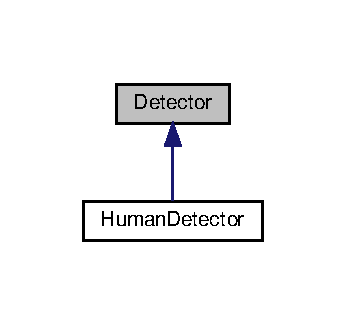
\includegraphics[width=166pt]{classDetector__inherit__graph}
\end{center}
\end{figure}
\subsection*{Public Member Functions}
\begin{DoxyCompactItemize}
\item 
\mbox{\Hypertarget{classDetector_afdf99890fb93a11252eef0dd85598c15}\label{classDetector_afdf99890fb93a11252eef0dd85598c15}} 
virtual std\+::vector$<$ Coord3D $>$ \hyperlink{classDetector_afdf99890fb93a11252eef0dd85598c15}{detect} (const cv\+::\+Mat \&input\+Data, bool is\+Test\+Mode)=0
\begin{DoxyCompactList}\small\item\em detects objects in image \end{DoxyCompactList}\item 
\mbox{\Hypertarget{classDetector_afaaefdcb9f6271dadf13fd2158e5d9be}\label{classDetector_afaaefdcb9f6271dadf13fd2158e5d9be}} 
virtual double {\bfseries evaluate\+Model} (const cv\+::\+Mat \&input\+Data, std\+::vector$<$ \hyperlink{structCentroid}{Centroid} $>$ gt\+\_\+centroids)=0
\end{DoxyCompactItemize}


\subsection{Detailed Description}
Generic object detection class. 

The documentation for this class was generated from the following file\+:\begin{DoxyCompactItemize}
\item 
include/\hyperlink{detector_8hpp}{detector.\+hpp}\end{DoxyCompactItemize}

\hypertarget{classDriver}{}\section{Driver Class Reference}
\label{classDriver}\index{Driver@{Driver}}


This class is responsible for executing the complete detection pipline.  




{\ttfamily \#include $<$driver.\+hpp$>$}

\subsection*{Public Member Functions}
\begin{DoxyCompactItemize}
\item 
\hyperlink{classDriver_af0658d103e3e810a8e9ef0a53bb2e261}{Driver} ()
\begin{DoxyCompactList}\small\item\em Construct a new \hyperlink{classDriver}{Driver} object. \end{DoxyCompactList}\item 
\hyperlink{classDriver_a6c9f75abe2410437cd3a0091d2ed41b3}{Driver} (std\+::unique\+\_\+ptr$<$ \hyperlink{classDataReader}{Data\+Reader}$<$ cv\+::\+Mat $>$$>$ data\+Reader, std\+::unique\+\_\+ptr$<$ \hyperlink{classPreProcessor}{Pre\+Processor} $>$ pre\+Processor, std\+::unique\+\_\+ptr$<$ \hyperlink{classDetector}{Detector} $>$ detector)
\begin{DoxyCompactList}\small\item\em Construct a new \hyperlink{classDriver}{Driver} object. \end{DoxyCompactList}\item 
\mbox{\Hypertarget{classDriver_ac7645eea8d3ce2bc39ddbda5e840297a}\label{classDriver_ac7645eea8d3ce2bc39ddbda5e840297a}} 
virtual \hyperlink{classDriver_ac7645eea8d3ce2bc39ddbda5e840297a}{$\sim$\+Driver} ()
\begin{DoxyCompactList}\small\item\em Destroy the \hyperlink{classDriver}{Driver} object. \end{DoxyCompactList}\item 
bool \hyperlink{classDriver_a33a612943ed1cbc375f0104a2a274b97}{execute\+Detection\+Pipe\+Line} (std\+::string data\+\_\+path)
\begin{DoxyCompactList}\small\item\em starts the detection flow given the path to the test data \end{DoxyCompactList}\end{DoxyCompactItemize}


\subsection{Detailed Description}
This class is responsible for executing the complete detection pipline. 

Copyright 2021 Sakshi Kakde, Siddharth Telang, Anubhav Paras 

\subsection{Constructor \& Destructor Documentation}
\mbox{\Hypertarget{classDriver_af0658d103e3e810a8e9ef0a53bb2e261}\label{classDriver_af0658d103e3e810a8e9ef0a53bb2e261}} 
\index{Driver@{Driver}!Driver@{Driver}}
\index{Driver@{Driver}!Driver@{Driver}}
\subsubsection{\texorpdfstring{Driver()}{Driver()}\hspace{0.1cm}{\footnotesize\ttfamily [1/2]}}
{\footnotesize\ttfamily Driver\+::\+Driver (\begin{DoxyParamCaption}{ }\end{DoxyParamCaption})}



Construct a new \hyperlink{classDriver}{Driver} object. 

Copyright 2021 Sakshi Kakde, Siddharth Telang, Anubhav Paras \mbox{\Hypertarget{classDriver_a6c9f75abe2410437cd3a0091d2ed41b3}\label{classDriver_a6c9f75abe2410437cd3a0091d2ed41b3}} 
\index{Driver@{Driver}!Driver@{Driver}}
\index{Driver@{Driver}!Driver@{Driver}}
\subsubsection{\texorpdfstring{Driver()}{Driver()}\hspace{0.1cm}{\footnotesize\ttfamily [2/2]}}
{\footnotesize\ttfamily Driver\+::\+Driver (\begin{DoxyParamCaption}\item[{std\+::unique\+\_\+ptr$<$ \hyperlink{classDataReader}{Data\+Reader}$<$ cv\+::\+Mat $>$$>$}]{data\+Reader,  }\item[{std\+::unique\+\_\+ptr$<$ \hyperlink{classPreProcessor}{Pre\+Processor} $>$}]{pre\+Processor,  }\item[{std\+::unique\+\_\+ptr$<$ \hyperlink{classDetector}{Detector} $>$}]{detector }\end{DoxyParamCaption})}



Construct a new \hyperlink{classDriver}{Driver} object. 


\begin{DoxyParams}{Parameters}
{\em data\+Reader} & to read the images or video/camera feed \\
\hline
{\em pre\+Processor} & for the preprocessing of the data \\
\hline
{\em detector} & to detect the objects in the image data \\
\hline
\end{DoxyParams}


\subsection{Member Function Documentation}
\mbox{\Hypertarget{classDriver_a33a612943ed1cbc375f0104a2a274b97}\label{classDriver_a33a612943ed1cbc375f0104a2a274b97}} 
\index{Driver@{Driver}!execute\+Detection\+Pipe\+Line@{execute\+Detection\+Pipe\+Line}}
\index{execute\+Detection\+Pipe\+Line@{execute\+Detection\+Pipe\+Line}!Driver@{Driver}}
\subsubsection{\texorpdfstring{execute\+Detection\+Pipe\+Line()}{executeDetectionPipeLine()}}
{\footnotesize\ttfamily bool Driver\+::execute\+Detection\+Pipe\+Line (\begin{DoxyParamCaption}\item[{std\+::string}]{data\+\_\+path }\end{DoxyParamCaption})}



starts the detection flow given the path to the test data 


\begin{DoxyParams}{Parameters}
{\em data\+\_\+path} & \\
\hline
\end{DoxyParams}


The documentation for this class was generated from the following files\+:\begin{DoxyCompactItemize}
\item 
include/driver.\+hpp\item 
src/driver.\+cpp\end{DoxyCompactItemize}

\hypertarget{classFrameTransformation}{}\section{Frame\+Transformation Class Reference}
\label{classFrameTransformation}\index{Frame\+Transformation@{Frame\+Transformation}}


Class responsible to convert the coordinates from camera frame to robot frame.  




{\ttfamily \#include $<$frame\+\_\+transformation.\+hpp$>$}

\subsection*{Public Member Functions}
\begin{DoxyCompactItemize}
\item 
\mbox{\Hypertarget{classFrameTransformation_aa4495bbd8e06ac1d793063c7a0aa0c03}\label{classFrameTransformation_aa4495bbd8e06ac1d793063c7a0aa0c03}} 
\hyperlink{classFrameTransformation_aa4495bbd8e06ac1d793063c7a0aa0c03}{Frame\+Transformation} ()
\begin{DoxyCompactList}\small\item\em Construct a new Frame Transformation object. \end{DoxyCompactList}\item 
\mbox{\Hypertarget{classFrameTransformation_a6db4d1bb1d72c02855aa2732205cd313}\label{classFrameTransformation_a6db4d1bb1d72c02855aa2732205cd313}} 
virtual \hyperlink{classFrameTransformation_a6db4d1bb1d72c02855aa2732205cd313}{$\sim$\+Frame\+Transformation} ()
\begin{DoxyCompactList}\small\item\em Destroy the Frame Transformation object. \end{DoxyCompactList}\item 
virtual Coord3D \hyperlink{classFrameTransformation_ab5131e1392b2fb97c65014eec96d54a8}{get\+Robot\+Frame} (Coord2D image\+Coordinates)
\begin{DoxyCompactList}\small\item\em Get the Robot Frame object. \end{DoxyCompactList}\end{DoxyCompactItemize}


\subsection{Detailed Description}
Class responsible to convert the coordinates from camera frame to robot frame. 

\subsection{Member Function Documentation}
\mbox{\Hypertarget{classFrameTransformation_ab5131e1392b2fb97c65014eec96d54a8}\label{classFrameTransformation_ab5131e1392b2fb97c65014eec96d54a8}} 
\index{Frame\+Transformation@{Frame\+Transformation}!get\+Robot\+Frame@{get\+Robot\+Frame}}
\index{get\+Robot\+Frame@{get\+Robot\+Frame}!Frame\+Transformation@{Frame\+Transformation}}
\subsubsection{\texorpdfstring{get\+Robot\+Frame()}{getRobotFrame()}}
{\footnotesize\ttfamily Coord3D Frame\+Transformation\+::get\+Robot\+Frame (\begin{DoxyParamCaption}\item[{Coord2D}]{image\+Coordinates }\end{DoxyParamCaption})\hspace{0.3cm}{\ttfamily [virtual]}}



Get the Robot Frame object. 


\begin{DoxyParams}{Parameters}
{\em image\+Coordinates} & coordinates in camera frame \\
\hline
\end{DoxyParams}
\begin{DoxyReturn}{Returns}
Coord3D coordinates in robot frame 
\end{DoxyReturn}


The documentation for this class was generated from the following files\+:\begin{DoxyCompactItemize}
\item 
include/\hyperlink{frame__transformation_8hpp}{frame\+\_\+transformation.\+hpp}\item 
src/\hyperlink{frame__transformation_8cpp}{frame\+\_\+transformation.\+cpp}\end{DoxyCompactItemize}

\hypertarget{classHumanDetector}{}\section{Human\+Detector Class Reference}
\label{classHumanDetector}\index{Human\+Detector@{Human\+Detector}}


Inheritance diagram for Human\+Detector\+:\nopagebreak
\begin{figure}[H]
\begin{center}
\leavevmode
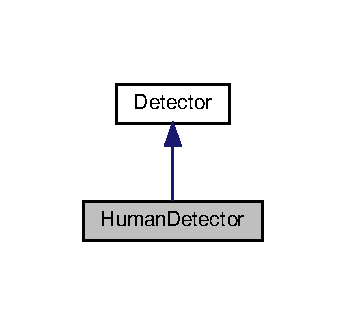
\includegraphics[width=166pt]{classHumanDetector__inherit__graph}
\end{center}
\end{figure}


Collaboration diagram for Human\+Detector\+:\nopagebreak
\begin{figure}[H]
\begin{center}
\leavevmode
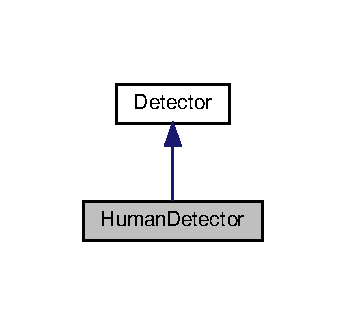
\includegraphics[width=166pt]{classHumanDetector__coll__graph}
\end{center}
\end{figure}
\subsection*{Public Member Functions}
\begin{DoxyCompactItemize}
\item 
\hyperlink{classHumanDetector_ad24009d2c6d212e037ee2ae46a9b9c05}{Human\+Detector} (std\+::unique\+\_\+ptr$<$ \hyperlink{classModel}{Model}$<$ \hyperlink{classData}{Detection\+Output}, Image $>$$>$ model, std\+::unique\+\_\+ptr$<$ \hyperlink{classFrameTransformation}{Frame\+Transformation} $>$ robot\+Frame)
\begin{DoxyCompactList}\small\item\em Construct a new Human \hyperlink{classDetector}{Detector} object. \end{DoxyCompactList}\item 
\mbox{\Hypertarget{classHumanDetector_a14a3f12c65510640240522c9e064b5f6}\label{classHumanDetector_a14a3f12c65510640240522c9e064b5f6}} 
\hyperlink{classHumanDetector_a14a3f12c65510640240522c9e064b5f6}{$\sim$\+Human\+Detector} ()
\begin{DoxyCompactList}\small\item\em Destroy the Human \hyperlink{classDetector}{Detector} object. \end{DoxyCompactList}\item 
std\+::vector$<$ Coord3D $>$ \hyperlink{classHumanDetector_ad6939ac83173d50f4420eae30ff3f978}{detect} (const cv\+::\+Mat \&input\+Data, bool is\+Test\+Mode) override
\begin{DoxyCompactList}\small\item\em detects the humans in a given image data displays the bounding boxes and the ids of all the humans detected \end{DoxyCompactList}\item 
double \hyperlink{classHumanDetector_af24d889a9b48029f405a0e6c105b898a}{evaluate\+Model} (const cv\+::\+Mat \&input\+Data, std\+::vector$<$ \hyperlink{structCentroid}{Centroid} $>$ gt\+\_\+centroids)
\begin{DoxyCompactList}\small\item\em evaluate the detection model based on the ground truth centroids \end{DoxyCompactList}\end{DoxyCompactItemize}


\subsection{Constructor \& Destructor Documentation}
\mbox{\Hypertarget{classHumanDetector_ad24009d2c6d212e037ee2ae46a9b9c05}\label{classHumanDetector_ad24009d2c6d212e037ee2ae46a9b9c05}} 
\index{Human\+Detector@{Human\+Detector}!Human\+Detector@{Human\+Detector}}
\index{Human\+Detector@{Human\+Detector}!Human\+Detector@{Human\+Detector}}
\subsubsection{\texorpdfstring{Human\+Detector()}{HumanDetector()}}
{\footnotesize\ttfamily H\+D\+::\+Human\+Detector (\begin{DoxyParamCaption}\item[{std\+::unique\+\_\+ptr$<$ \hyperlink{classModel}{Model}$<$ \hyperlink{classData}{Detection\+Output}, Image $>$$>$}]{model,  }\item[{std\+::unique\+\_\+ptr$<$ \hyperlink{classFrameTransformation}{Frame\+Transformation} $>$}]{robot\+Frame }\end{DoxyParamCaption})}



Construct a new Human \hyperlink{classDetector}{Detector} object. 


\begin{DoxyParams}{Parameters}
{\em model} & model used to predict and fetch the bounding boxes \\
\hline
{\em robot\+Frame} & frame transformation to get the coordinates in robot frame \\
\hline
\end{DoxyParams}


\subsection{Member Function Documentation}
\mbox{\Hypertarget{classHumanDetector_ad6939ac83173d50f4420eae30ff3f978}\label{classHumanDetector_ad6939ac83173d50f4420eae30ff3f978}} 
\index{Human\+Detector@{Human\+Detector}!detect@{detect}}
\index{detect@{detect}!Human\+Detector@{Human\+Detector}}
\subsubsection{\texorpdfstring{detect()}{detect()}}
{\footnotesize\ttfamily std\+::vector$<$ Coord3D $>$ H\+D\+::detect (\begin{DoxyParamCaption}\item[{const cv\+::\+Mat \&}]{input\+Data,  }\item[{bool}]{is\+Test\+Mode }\end{DoxyParamCaption})\hspace{0.3cm}{\ttfamily [override]}, {\ttfamily [virtual]}}



detects the humans in a given image data displays the bounding boxes and the ids of all the humans detected 


\begin{DoxyParams}{Parameters}
{\em input\+Data} & input image data \\
\hline
{\em is\+Test\+Mode} & to check if detect is being called while unit testing \\
\hline
\end{DoxyParams}
\begin{DoxyReturn}{Returns}
std\+::vector$<$\+Coord3\+D$>$ coordinates of all the detected humans in robot frame 
\end{DoxyReturn}


Implements \hyperlink{classDetector_afdf99890fb93a11252eef0dd85598c15}{Detector}.

\mbox{\Hypertarget{classHumanDetector_af24d889a9b48029f405a0e6c105b898a}\label{classHumanDetector_af24d889a9b48029f405a0e6c105b898a}} 
\index{Human\+Detector@{Human\+Detector}!evaluate\+Model@{evaluate\+Model}}
\index{evaluate\+Model@{evaluate\+Model}!Human\+Detector@{Human\+Detector}}
\subsubsection{\texorpdfstring{evaluate\+Model()}{evaluateModel()}}
{\footnotesize\ttfamily double H\+D\+::evaluate\+Model (\begin{DoxyParamCaption}\item[{const cv\+::\+Mat \&}]{input\+Data,  }\item[{std\+::vector$<$ \hyperlink{structCentroid}{Centroid} $>$}]{gt\+\_\+centroids }\end{DoxyParamCaption})\hspace{0.3cm}{\ttfamily [virtual]}}



evaluate the detection model based on the ground truth centroids 


\begin{DoxyParams}{Parameters}
{\em input\+Data} & input image data \\
\hline
{\em gt\+\_\+centroids} & vector of ground truth centroid values for all the detected humans \\
\hline
\end{DoxyParams}
\begin{DoxyReturn}{Returns}
double average error in the centroids of the detected bounding boxes 
\end{DoxyReturn}


Implements \hyperlink{classDetector}{Detector}.



The documentation for this class was generated from the following files\+:\begin{DoxyCompactItemize}
\item 
include/\hyperlink{detector_8hpp}{detector.\+hpp}\item 
src/\hyperlink{detector_8cpp}{detector.\+cpp}\end{DoxyCompactItemize}

\hypertarget{classImageReader}{}\section{Image\+Reader Class Reference}
\label{classImageReader}\index{Image\+Reader@{Image\+Reader}}


Inheritance diagram for Image\+Reader\+:
\nopagebreak
\begin{figure}[H]
\begin{center}
\leavevmode
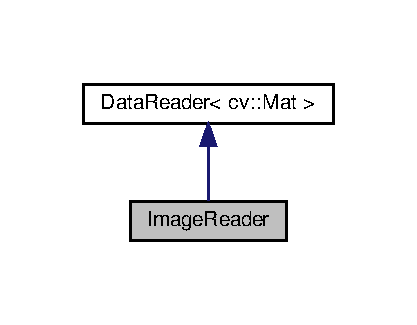
\includegraphics[width=200pt]{classImageReader__inherit__graph}
\end{center}
\end{figure}


Collaboration diagram for Image\+Reader\+:
\nopagebreak
\begin{figure}[H]
\begin{center}
\leavevmode
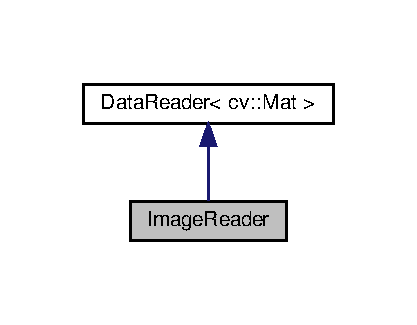
\includegraphics[width=200pt]{classImageReader__coll__graph}
\end{center}
\end{figure}
\subsection*{Public Member Functions}
\begin{DoxyCompactItemize}
\item 
\hyperlink{classImageReader_a2b24331603b06f5c218212c26a3ee24b}{Image\+Reader} ()
\begin{DoxyCompactList}\small\item\em Construct a new Image Reader object. \end{DoxyCompactList}\item 
\mbox{\Hypertarget{classImageReader_a4d5b604cbc552bd86d9ec357139fd61e}\label{classImageReader_a4d5b604cbc552bd86d9ec357139fd61e}} 
\hyperlink{classImageReader_a4d5b604cbc552bd86d9ec357139fd61e}{$\sim$\+Image\+Reader} ()
\begin{DoxyCompactList}\small\item\em Destroy the Image Reader object. \end{DoxyCompactList}\item 
cv\+::\+Mat \hyperlink{classImageReader_a453f68fc55ae911476514068873f9a3f}{read\+Data} (std\+::string path=\char`\"{}\char`\"{}) override
\begin{DoxyCompactList}\small\item\em read the image type data from given string path \end{DoxyCompactList}\end{DoxyCompactItemize}


\subsection{Constructor \& Destructor Documentation}
\mbox{\Hypertarget{classImageReader_a2b24331603b06f5c218212c26a3ee24b}\label{classImageReader_a2b24331603b06f5c218212c26a3ee24b}} 
\index{Image\+Reader@{Image\+Reader}!Image\+Reader@{Image\+Reader}}
\index{Image\+Reader@{Image\+Reader}!Image\+Reader@{Image\+Reader}}
\subsubsection{\texorpdfstring{Image\+Reader()}{ImageReader()}}
{\footnotesize\ttfamily Image\+Reader\+::\+Image\+Reader (\begin{DoxyParamCaption}{ }\end{DoxyParamCaption})}



Construct a new Image Reader object. 

Copyright 2021 Sakshi Kakde, Siddharth Telang, Anubhav Paras 

\subsection{Member Function Documentation}
\mbox{\Hypertarget{classImageReader_a453f68fc55ae911476514068873f9a3f}\label{classImageReader_a453f68fc55ae911476514068873f9a3f}} 
\index{Image\+Reader@{Image\+Reader}!read\+Data@{read\+Data}}
\index{read\+Data@{read\+Data}!Image\+Reader@{Image\+Reader}}
\subsubsection{\texorpdfstring{read\+Data()}{readData()}}
{\footnotesize\ttfamily cv\+::\+Mat Image\+Reader\+::read\+Data (\begin{DoxyParamCaption}\item[{std\+::string}]{path = {\ttfamily \char`\"{}\char`\"{}} }\end{DoxyParamCaption})\hspace{0.3cm}{\ttfamily [override]}, {\ttfamily [virtual]}}



read the image type data from given string path 


\begin{DoxyParams}{Parameters}
{\em path} & location of the image file \\
\hline
\end{DoxyParams}
\begin{DoxyReturn}{Returns}
cv\+::\+Mat output frame 
\end{DoxyReturn}


Implements \hyperlink{classDataReader}{Data\+Reader$<$ cv\+::\+Mat $>$}.



The documentation for this class was generated from the following files\+:\begin{DoxyCompactItemize}
\item 
include/datareader.\+hpp\item 
src/datareader.\+cpp\end{DoxyCompactItemize}

\hypertarget{classModel}{}\section{Model$<$ T, U $>$ Class Template Reference}
\label{classModel}\index{Model$<$ T, U $>$@{Model$<$ T, U $>$}}


Abstract \hyperlink{classModel}{Model} class for all the ML models.  




{\ttfamily \#include $<$model.\+hpp$>$}

\subsection*{Public Member Functions}
\begin{DoxyCompactItemize}
\item 
virtual T \hyperlink{classModel_aab70aeca992eb3a1ce09667e169b8743}{predict} (U data)=0
\begin{DoxyCompactList}\small\item\em model to predict and return data of type T for any given input of type U \end{DoxyCompactList}\item 
\mbox{\Hypertarget{classModel_aa0a39659d8fc19ec48f2d83683567e05}\label{classModel_aa0a39659d8fc19ec48f2d83683567e05}} 
virtual \hyperlink{classModel_aa0a39659d8fc19ec48f2d83683567e05}{$\sim$\+Model} ()
\begin{DoxyCompactList}\small\item\em Destroy the \hyperlink{classModel}{Model} object. \end{DoxyCompactList}\end{DoxyCompactItemize}


\subsection{Detailed Description}
\subsubsection*{template$<$class T, class U$>$\newline
class Model$<$ T, U $>$}

Abstract \hyperlink{classModel}{Model} class for all the ML models. 


\begin{DoxyTemplParams}{Template Parameters}
{\em T} & return type of the prediction data \\
\hline
{\em U} & type of the input data used for prediction \\
\hline
\end{DoxyTemplParams}


\subsection{Member Function Documentation}
\mbox{\Hypertarget{classModel_aab70aeca992eb3a1ce09667e169b8743}\label{classModel_aab70aeca992eb3a1ce09667e169b8743}} 
\index{Model@{Model}!predict@{predict}}
\index{predict@{predict}!Model@{Model}}
\subsubsection{\texorpdfstring{predict()}{predict()}}
{\footnotesize\ttfamily template$<$class T, class U$>$ \\
virtual T \hyperlink{classModel}{Model}$<$ T, U $>$\+::predict (\begin{DoxyParamCaption}\item[{U}]{data }\end{DoxyParamCaption})\hspace{0.3cm}{\ttfamily [pure virtual]}}



model to predict and return data of type T for any given input of type U 


\begin{DoxyParams}{Parameters}
{\em data} & input data of type T for the prediction task \\
\hline
\end{DoxyParams}
\begin{DoxyReturn}{Returns}
T prediction data of type U 
\end{DoxyReturn}


Implemented in \hyperlink{classSVMHumanClassifier_a14a416a22355b1426d7611082dfa2464}{S\+V\+M\+Human\+Classifier}.



The documentation for this class was generated from the following file\+:\begin{DoxyCompactItemize}
\item 
include/\hyperlink{model_8hpp}{model.\+hpp}\end{DoxyCompactItemize}

\hypertarget{classPreProcessor}{}\section{Pre\+Processor Class Reference}
\label{classPreProcessor}\index{Pre\+Processor@{Pre\+Processor}}


Class to do all the preprocessing of the data.  




{\ttfamily \#include $<$preprocessor.\+hpp$>$}

\subsection*{Public Member Functions}
\begin{DoxyCompactItemize}
\item 
\hyperlink{classPreProcessor_ab0196882f25fc9aff349f4669d35de22}{Pre\+Processor} ()
\begin{DoxyCompactList}\small\item\em Construct a new Pre Processor object. \end{DoxyCompactList}\item 
\mbox{\Hypertarget{classPreProcessor_a5f0d6e2fd5982f2c5f197035beaeed6b}\label{classPreProcessor_a5f0d6e2fd5982f2c5f197035beaeed6b}} 
virtual \hyperlink{classPreProcessor_a5f0d6e2fd5982f2c5f197035beaeed6b}{$\sim$\+Pre\+Processor} ()
\begin{DoxyCompactList}\small\item\em Destroy the Pre Processor object. \end{DoxyCompactList}\item 
virtual void \hyperlink{classPreProcessor_a49b49d13b2422e02ff7817e965d174df}{resize} (cv\+::\+Input\+Array input, cv\+::\+Output\+Array output, cv\+::\+Size size)
\end{DoxyCompactItemize}


\subsection{Detailed Description}
Class to do all the preprocessing of the data. 

Copyright 2021 Sakshi Kakde, Siddharth Telang, Anubhav Paras 

\subsection{Constructor \& Destructor Documentation}
\mbox{\Hypertarget{classPreProcessor_ab0196882f25fc9aff349f4669d35de22}\label{classPreProcessor_ab0196882f25fc9aff349f4669d35de22}} 
\index{Pre\+Processor@{Pre\+Processor}!Pre\+Processor@{Pre\+Processor}}
\index{Pre\+Processor@{Pre\+Processor}!Pre\+Processor@{Pre\+Processor}}
\subsubsection{\texorpdfstring{Pre\+Processor()}{PreProcessor()}}
{\footnotesize\ttfamily Pre\+Processor\+::\+Pre\+Processor (\begin{DoxyParamCaption}{ }\end{DoxyParamCaption})}



Construct a new Pre Processor object. 

Copyright 2021 Sakshi Kakde, Siddharth Telang, Anubhav Paras 

\subsection{Member Function Documentation}
\mbox{\Hypertarget{classPreProcessor_a49b49d13b2422e02ff7817e965d174df}\label{classPreProcessor_a49b49d13b2422e02ff7817e965d174df}} 
\index{Pre\+Processor@{Pre\+Processor}!resize@{resize}}
\index{resize@{resize}!Pre\+Processor@{Pre\+Processor}}
\subsubsection{\texorpdfstring{resize()}{resize()}}
{\footnotesize\ttfamily void Pre\+Processor\+::resize (\begin{DoxyParamCaption}\item[{cv\+::\+Input\+Array}]{input,  }\item[{cv\+::\+Output\+Array}]{output,  }\item[{cv\+::\+Size}]{size }\end{DoxyParamCaption})\hspace{0.3cm}{\ttfamily [virtual]}}


\begin{DoxyParams}{Parameters}
{\em input} & \\
\hline
{\em output} & \\
\hline
{\em size} & \\
\hline
\end{DoxyParams}


The documentation for this class was generated from the following files\+:\begin{DoxyCompactItemize}
\item 
include/preprocessor.\+hpp\item 
src/preprocessor.\+cpp\end{DoxyCompactItemize}

\hypertarget{classSVMHumanClassifier}{}\section{S\+V\+M\+Human\+Classifier Class Reference}
\label{classSVMHumanClassifier}\index{S\+V\+M\+Human\+Classifier@{S\+V\+M\+Human\+Classifier}}


Inheritance diagram for S\+V\+M\+Human\+Classifier\+:
\nopagebreak
\begin{figure}[H]
\begin{center}
\leavevmode
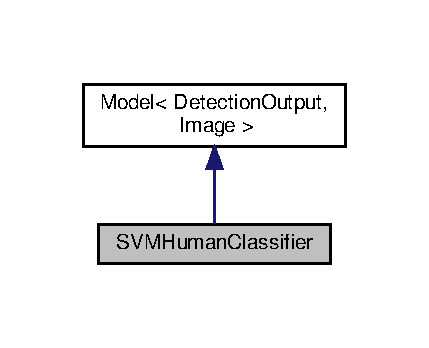
\includegraphics[width=206pt]{classSVMHumanClassifier__inherit__graph}
\end{center}
\end{figure}


Collaboration diagram for S\+V\+M\+Human\+Classifier\+:
\nopagebreak
\begin{figure}[H]
\begin{center}
\leavevmode
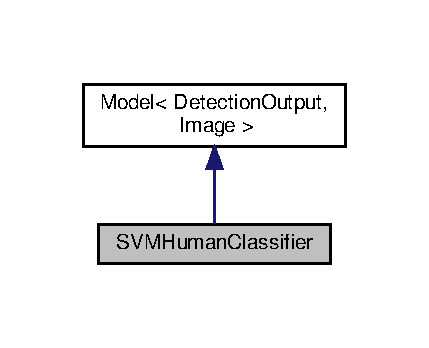
\includegraphics[width=206pt]{classSVMHumanClassifier__coll__graph}
\end{center}
\end{figure}
\subsection*{Public Member Functions}
\begin{DoxyCompactItemize}
\item 
\hyperlink{classSVMHumanClassifier_ab99099674465b0ffa8c79feeb9b9b66a}{S\+V\+M\+Human\+Classifier} ()
\begin{DoxyCompactList}\small\item\em Construct a new \hyperlink{classSVMHumanClassifier}{S\+V\+M\+Human\+Classifier} object. \end{DoxyCompactList}\item 
virtual \hyperlink{classSVMHumanClassifier_a875ce0f61e85c8254f008b29f2c3a9b9}{$\sim$\+S\+V\+M\+Human\+Classifier} ()
\begin{DoxyCompactList}\small\item\em Parameterized constructur to construct new \hyperlink{classSVMHumanClassifier}{S\+V\+M\+Human\+Classifier} object. \end{DoxyCompactList}\item 
\hyperlink{classData}{Detection\+Output} \hyperlink{classSVMHumanClassifier_a14a416a22355b1426d7611082dfa2464}{predict} (Image input\+Data) override
\begin{DoxyCompactList}\small\item\em predicts the classification output Takes an input image an returns the bounding boxes for the detected humans \end{DoxyCompactList}\end{DoxyCompactItemize}


\subsection{Constructor \& Destructor Documentation}
\mbox{\Hypertarget{classSVMHumanClassifier_ab99099674465b0ffa8c79feeb9b9b66a}\label{classSVMHumanClassifier_ab99099674465b0ffa8c79feeb9b9b66a}} 
\index{S\+V\+M\+Human\+Classifier@{S\+V\+M\+Human\+Classifier}!S\+V\+M\+Human\+Classifier@{S\+V\+M\+Human\+Classifier}}
\index{S\+V\+M\+Human\+Classifier@{S\+V\+M\+Human\+Classifier}!S\+V\+M\+Human\+Classifier@{S\+V\+M\+Human\+Classifier}}
\subsubsection{\texorpdfstring{S\+V\+M\+Human\+Classifier()}{SVMHumanClassifier()}}
{\footnotesize\ttfamily S\+V\+M\+Human\+Classifier\+::\+S\+V\+M\+Human\+Classifier (\begin{DoxyParamCaption}{ }\end{DoxyParamCaption})}



Construct a new \hyperlink{classSVMHumanClassifier}{S\+V\+M\+Human\+Classifier} object. 

Copyright 2021 Sakshi Kakde, Siddharth Telang, Anubhav Paras \mbox{\Hypertarget{classSVMHumanClassifier_a875ce0f61e85c8254f008b29f2c3a9b9}\label{classSVMHumanClassifier_a875ce0f61e85c8254f008b29f2c3a9b9}} 
\index{S\+V\+M\+Human\+Classifier@{S\+V\+M\+Human\+Classifier}!````~S\+V\+M\+Human\+Classifier@{$\sim$\+S\+V\+M\+Human\+Classifier}}
\index{````~S\+V\+M\+Human\+Classifier@{$\sim$\+S\+V\+M\+Human\+Classifier}!S\+V\+M\+Human\+Classifier@{S\+V\+M\+Human\+Classifier}}
\subsubsection{\texorpdfstring{$\sim$\+S\+V\+M\+Human\+Classifier()}{~SVMHumanClassifier()}}
{\footnotesize\ttfamily S\+V\+M\+Human\+Classifier\+::$\sim$\+S\+V\+M\+Human\+Classifier (\begin{DoxyParamCaption}{ }\end{DoxyParamCaption})\hspace{0.3cm}{\ttfamily [virtual]}}



Parameterized constructur to construct new \hyperlink{classSVMHumanClassifier}{S\+V\+M\+Human\+Classifier} object. 


\begin{DoxyParams}{Parameters}
{\em base\+Model} & base S\+VM model to Destroy the \hyperlink{classSVMHumanClassifier}{S\+V\+M\+Human\+Classifier} object \\
\hline
\end{DoxyParams}


\subsection{Member Function Documentation}
\mbox{\Hypertarget{classSVMHumanClassifier_a14a416a22355b1426d7611082dfa2464}\label{classSVMHumanClassifier_a14a416a22355b1426d7611082dfa2464}} 
\index{S\+V\+M\+Human\+Classifier@{S\+V\+M\+Human\+Classifier}!predict@{predict}}
\index{predict@{predict}!S\+V\+M\+Human\+Classifier@{S\+V\+M\+Human\+Classifier}}
\subsubsection{\texorpdfstring{predict()}{predict()}}
{\footnotesize\ttfamily \hyperlink{classData}{Detection\+Output} S\+V\+M\+Human\+Classifier\+::predict (\begin{DoxyParamCaption}\item[{Image}]{input\+Data }\end{DoxyParamCaption})\hspace{0.3cm}{\ttfamily [override]}, {\ttfamily [virtual]}}



predicts the classification output Takes an input image an returns the bounding boxes for the detected humans 


\begin{DoxyParams}{Parameters}
{\em input\+Data} & input image data \\
\hline
\end{DoxyParams}
\begin{DoxyReturn}{Returns}
Rectangles bounding boxes for all the humans detected 
\end{DoxyReturn}


Implements \hyperlink{classModel_aab70aeca992eb3a1ce09667e169b8743}{Model$<$ Detection\+Output, Image $>$}.



The documentation for this class was generated from the following files\+:\begin{DoxyCompactItemize}
\item 
include/model.\+hpp\item 
src/model.\+cpp\end{DoxyCompactItemize}

\chapter{File Documentation}
\hypertarget{data_8hpp}{}\section{include/data.hpp File Reference}
\label{data_8hpp}\index{include/data.\+hpp@{include/data.\+hpp}}


header file for \hyperlink{data_8cpp}{data.\+cpp}  


This graph shows which files directly or indirectly include this file\+:
\nopagebreak
\begin{figure}[H]
\begin{center}
\leavevmode
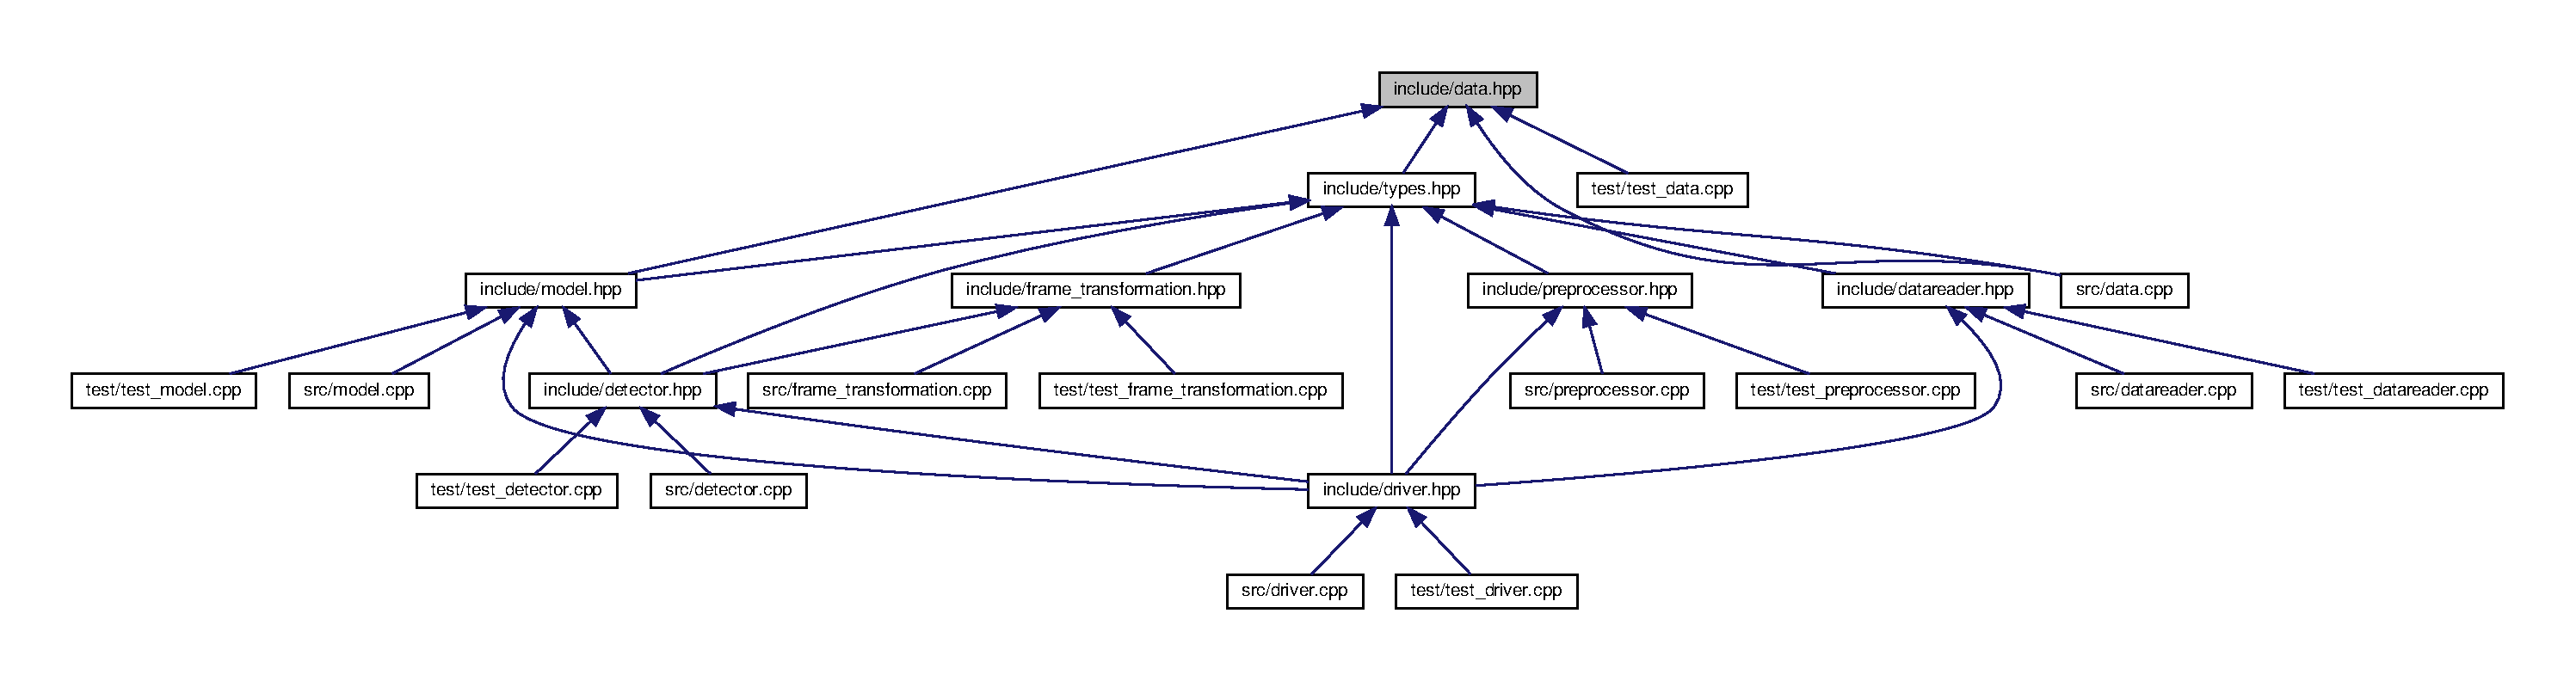
\includegraphics[width=350pt]{data_8hpp__dep__incl}
\end{center}
\end{figure}
\subsection*{Classes}
\begin{DoxyCompactItemize}
\item 
class \hyperlink{classData}{Data$<$ T $>$}
\begin{DoxyCompactList}\small\item\em Wrapper class for any encapsulate any datatype object. \end{DoxyCompactList}\end{DoxyCompactItemize}


\subsection{Detailed Description}
header file for \hyperlink{data_8cpp}{data.\+cpp} 

M\+IT License

Copyright (c) 2021 Anubhav Paras, Sakshi Kakde, Siddharth Telang

Permission is hereby granted, free of charge, to any person obtaining a copy of this software and associated documentation files (the \char`\"{}\+Software\char`\"{}), to deal in the Software without restriction, including without limitation the rights to use, copy, modify, merge, publish, distribute, sublicense, and/or sell copies of the Software, and to permit persons to whom the Software is furnished to do so, subject to the following conditions\+:

The above copyright notice and this permission notice shall be included in all copies or substantial portions of the Software.

T\+HE S\+O\+F\+T\+W\+A\+RE IS P\+R\+O\+V\+I\+D\+ED \char`\"{}\+A\+S I\+S\char`\"{}, W\+I\+T\+H\+O\+UT W\+A\+R\+R\+A\+N\+TY OF A\+NY K\+I\+ND, E\+X\+P\+R\+E\+SS OR I\+M\+P\+L\+I\+ED, I\+N\+C\+L\+U\+D\+I\+NG B\+UT N\+OT L\+I\+M\+I\+T\+ED TO T\+HE W\+A\+R\+R\+A\+N\+T\+I\+ES OF M\+E\+R\+C\+H\+A\+N\+T\+A\+B\+I\+L\+I\+TY, F\+I\+T\+N\+E\+SS F\+OR A P\+A\+R\+T\+I\+C\+U\+L\+AR P\+U\+R\+P\+O\+SE A\+ND N\+O\+N\+I\+N\+F\+R\+I\+N\+G\+E\+M\+E\+NT. IN NO E\+V\+E\+NT S\+H\+A\+LL T\+HE A\+U\+T\+H\+O\+RS OR C\+O\+P\+Y\+R\+I\+G\+HT H\+O\+L\+D\+E\+RS BE L\+I\+A\+B\+LE F\+OR A\+NY C\+L\+A\+IM, D\+A\+M\+A\+G\+ES OR O\+T\+H\+ER L\+I\+A\+B\+I\+L\+I\+TY, W\+H\+E\+T\+H\+ER IN AN A\+C\+T\+I\+ON OF C\+O\+N\+T\+R\+A\+CT, T\+O\+RT OR O\+T\+H\+E\+R\+W\+I\+SE, A\+R\+I\+S\+I\+NG F\+R\+OM, O\+UT OF OR IN C\+O\+N\+N\+E\+C\+T\+I\+ON W\+I\+TH T\+HE S\+O\+F\+T\+W\+A\+RE OR T\+HE U\+SE OR O\+T\+H\+ER D\+E\+A\+L\+I\+N\+GS IN T\+HE S\+O\+F\+T\+W\+A\+RE.

\begin{DoxyAuthor}{Author}
Anubhav Paras (\href{mailto:anubhav@umd.edu}{\tt anubhav@umd.\+edu}) 

Sakshi Kakde (\href{mailto:sakshi@umd.edu}{\tt sakshi@umd.\+edu}) 

Siddharth Telang (\href{mailto:stelang@umd.edu}{\tt stelang@umd.\+edu}) 
\end{DoxyAuthor}
\begin{DoxyVersion}{Version}
0.\+1 
\end{DoxyVersion}
\begin{DoxyDate}{Date}
2021-\/10-\/25
\end{DoxyDate}
\begin{DoxyCopyright}{Copyright}
Copyright (c) 2021 
\end{DoxyCopyright}

\hypertarget{datareader_8hpp}{}\section{include/datareader.hpp File Reference}
\label{datareader_8hpp}\index{include/datareader.\+hpp@{include/datareader.\+hpp}}


header file for \hyperlink{datareader_8cpp}{datareader.\+cpp}  


{\ttfamily \#include $<$memory$>$}\newline
{\ttfamily \#include $<$string$>$}\newline
{\ttfamily \#include $<$opencv2/opencv.\+hpp$>$}\newline
{\ttfamily \#include $<$types.\+hpp$>$}\newline
Include dependency graph for datareader.\+hpp\+:
\nopagebreak
\begin{figure}[H]
\begin{center}
\leavevmode
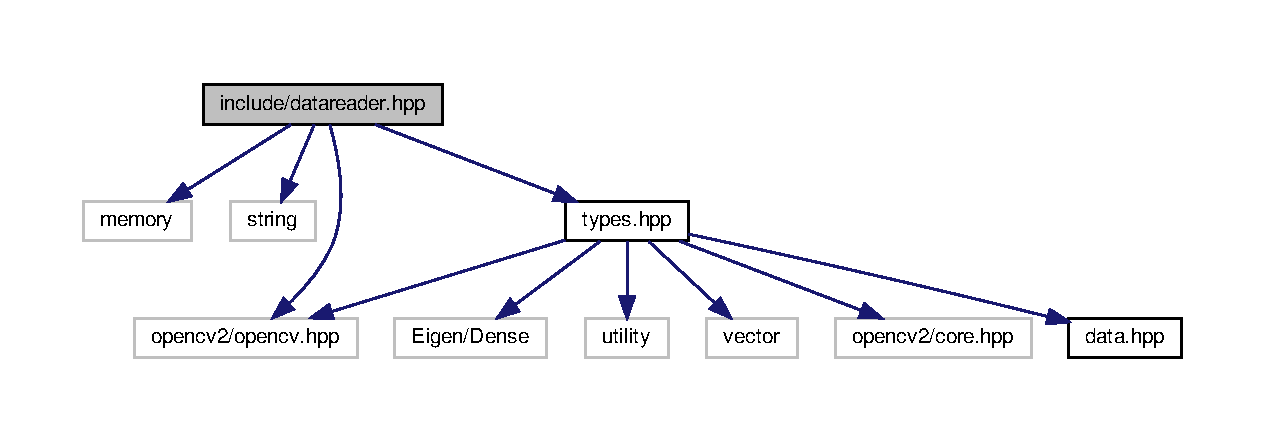
\includegraphics[width=350pt]{datareader_8hpp__incl}
\end{center}
\end{figure}
This graph shows which files directly or indirectly include this file\+:
\nopagebreak
\begin{figure}[H]
\begin{center}
\leavevmode
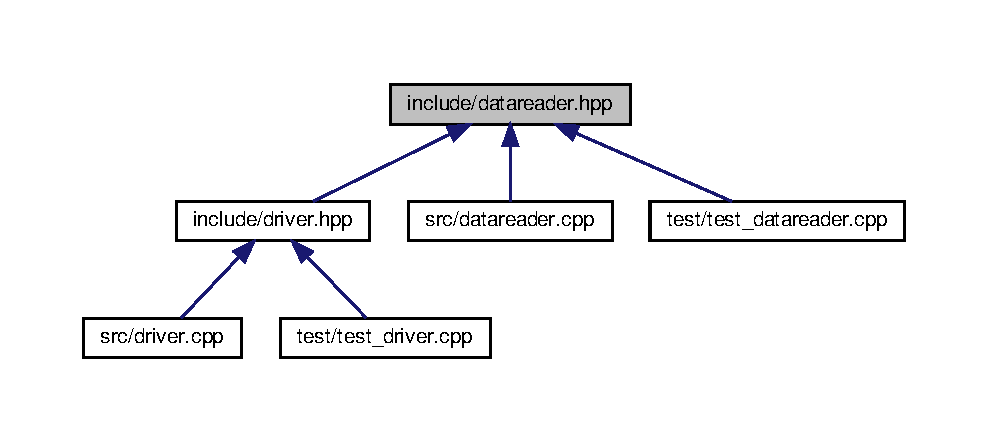
\includegraphics[width=350pt]{datareader_8hpp__dep__incl}
\end{center}
\end{figure}
\subsection*{Classes}
\begin{DoxyCompactItemize}
\item 
class \hyperlink{classDataReader}{Data\+Reader$<$ T, U $>$}
\begin{DoxyCompactList}\small\item\em Generic datareader class. \end{DoxyCompactList}\item 
class \hyperlink{classImageReader}{Image\+Reader}
\end{DoxyCompactItemize}


\subsection{Detailed Description}
header file for \hyperlink{datareader_8cpp}{datareader.\+cpp} 

M\+IT License

Copyright (c) 2021 Anubhav Paras, Sakshi Kakde, Siddharth Telang

Permission is hereby granted, free of charge, to any person obtaining a copy of this software and associated documentation files (the \char`\"{}\+Software\char`\"{}), to deal in the Software without restriction, including without limitation the rights to use, copy, modify, merge, publish, distribute, sublicense, and/or sell copies of the Software, and to permit persons to whom the Software is furnished to do so, subject to the following conditions\+:

The above copyright notice and this permission notice shall be included in all copies or substantial portions of the Software.

T\+HE S\+O\+F\+T\+W\+A\+RE IS P\+R\+O\+V\+I\+D\+ED \char`\"{}\+A\+S I\+S\char`\"{}, W\+I\+T\+H\+O\+UT W\+A\+R\+R\+A\+N\+TY OF A\+NY K\+I\+ND, E\+X\+P\+R\+E\+SS OR I\+M\+P\+L\+I\+ED, I\+N\+C\+L\+U\+D\+I\+NG B\+UT N\+OT L\+I\+M\+I\+T\+ED TO T\+HE W\+A\+R\+R\+A\+N\+T\+I\+ES OF M\+E\+R\+C\+H\+A\+N\+T\+A\+B\+I\+L\+I\+TY, F\+I\+T\+N\+E\+SS F\+OR A P\+A\+R\+T\+I\+C\+U\+L\+AR P\+U\+R\+P\+O\+SE A\+ND N\+O\+N\+I\+N\+F\+R\+I\+N\+G\+E\+M\+E\+NT. IN NO E\+V\+E\+NT S\+H\+A\+LL T\+HE A\+U\+T\+H\+O\+RS OR C\+O\+P\+Y\+R\+I\+G\+HT H\+O\+L\+D\+E\+RS BE L\+I\+A\+B\+LE F\+OR A\+NY C\+L\+A\+IM, D\+A\+M\+A\+G\+ES OR O\+T\+H\+ER L\+I\+A\+B\+I\+L\+I\+TY, W\+H\+E\+T\+H\+ER IN AN A\+C\+T\+I\+ON OF C\+O\+N\+T\+R\+A\+CT, T\+O\+RT OR O\+T\+H\+E\+R\+W\+I\+SE, A\+R\+I\+S\+I\+NG F\+R\+OM, O\+UT OF OR IN C\+O\+N\+N\+E\+C\+T\+I\+ON W\+I\+TH T\+HE S\+O\+F\+T\+W\+A\+RE OR T\+HE U\+SE OR O\+T\+H\+ER D\+E\+A\+L\+I\+N\+GS IN T\+HE S\+O\+F\+T\+W\+A\+RE.

\begin{DoxyAuthor}{Author}
Anubhav Paras (\href{mailto:anubhav@umd.edu}{\tt anubhav@umd.\+edu}) 

Sakshi Kakde (\href{mailto:sakshi@umd.edu}{\tt sakshi@umd.\+edu}) 

Siddharth Telang (\href{mailto:stelang@umd.edu}{\tt stelang@umd.\+edu}) 
\end{DoxyAuthor}
\begin{DoxyVersion}{Version}
0.\+1 
\end{DoxyVersion}
\begin{DoxyDate}{Date}
2021-\/10-\/25
\end{DoxyDate}
\begin{DoxyCopyright}{Copyright}
Copyright (c) 2021 
\end{DoxyCopyright}

\hypertarget{detector_8hpp}{}\section{include/detector.hpp File Reference}
\label{detector_8hpp}\index{include/detector.\+hpp@{include/detector.\+hpp}}


header file for \hyperlink{detector_8cpp}{detector.\+cpp}  


{\ttfamily \#include $<$memory$>$}\newline
{\ttfamily \#include $<$vector$>$}\newline
{\ttfamily \#include $<$model.\+hpp$>$}\newline
{\ttfamily \#include $<$frame\+\_\+transformation.\+hpp$>$}\newline
{\ttfamily \#include $<$types.\+hpp$>$}\newline
Include dependency graph for detector.\+hpp\+:
\nopagebreak
\begin{figure}[H]
\begin{center}
\leavevmode
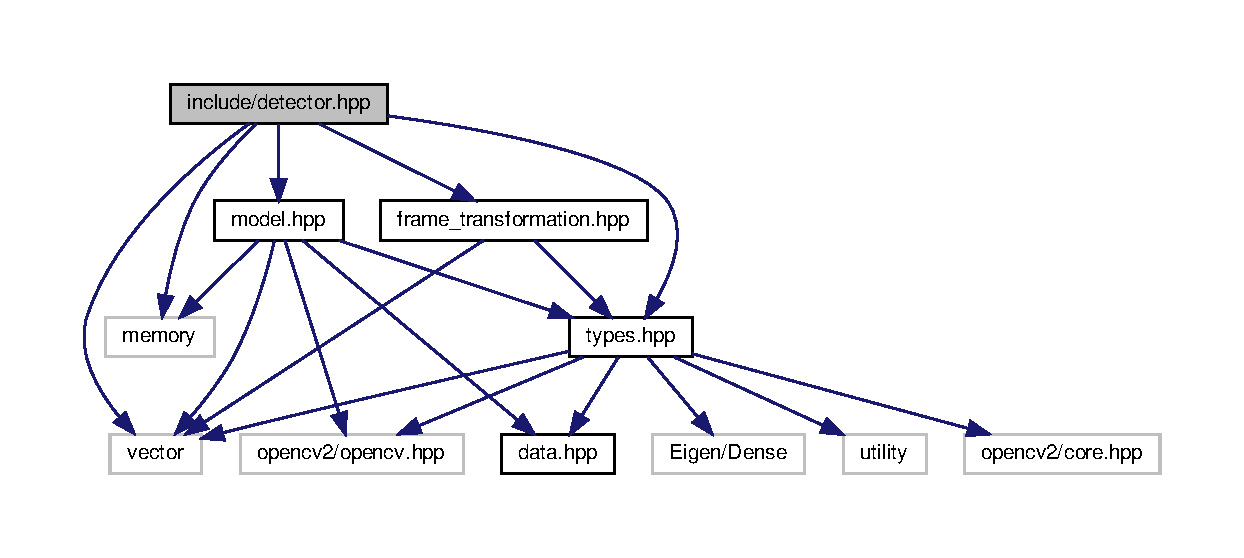
\includegraphics[width=350pt]{detector_8hpp__incl}
\end{center}
\end{figure}
This graph shows which files directly or indirectly include this file\+:
\nopagebreak
\begin{figure}[H]
\begin{center}
\leavevmode
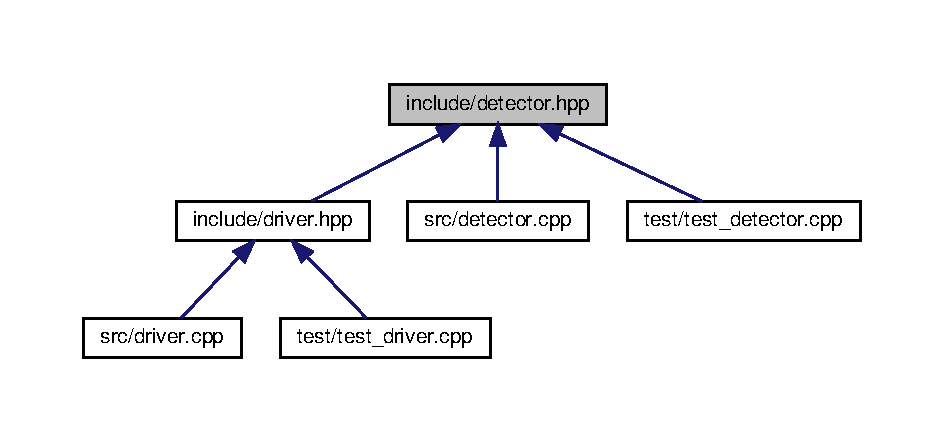
\includegraphics[width=350pt]{detector_8hpp__dep__incl}
\end{center}
\end{figure}
\subsection*{Classes}
\begin{DoxyCompactItemize}
\item 
class \hyperlink{classDetector}{Detector}
\begin{DoxyCompactList}\small\item\em Generic object detection class. \end{DoxyCompactList}\item 
class \hyperlink{classHumanDetector}{Human\+Detector}
\end{DoxyCompactItemize}


\subsection{Detailed Description}
header file for \hyperlink{detector_8cpp}{detector.\+cpp} 

M\+IT License

Copyright (c) 2021 Anubhav Paras, Sakshi Kakde, Siddharth Telang

Permission is hereby granted, free of charge, to any person obtaining a copy of this software and associated documentation files (the \char`\"{}\+Software\char`\"{}), to deal in the Software without restriction, including without limitation the rights to use, copy, modify, merge, publish, distribute, sublicense, and/or sell copies of the Software, and to permit persons to whom the Software is furnished to do so, subject to the following conditions\+:

The above copyright notice and this permission notice shall be included in all copies or substantial portions of the Software.

T\+HE S\+O\+F\+T\+W\+A\+RE IS P\+R\+O\+V\+I\+D\+ED \char`\"{}\+A\+S I\+S\char`\"{}, W\+I\+T\+H\+O\+UT W\+A\+R\+R\+A\+N\+TY OF A\+NY K\+I\+ND, E\+X\+P\+R\+E\+SS OR I\+M\+P\+L\+I\+ED, I\+N\+C\+L\+U\+D\+I\+NG B\+UT N\+OT L\+I\+M\+I\+T\+ED TO T\+HE W\+A\+R\+R\+A\+N\+T\+I\+ES OF M\+E\+R\+C\+H\+A\+N\+T\+A\+B\+I\+L\+I\+TY, F\+I\+T\+N\+E\+SS F\+OR A P\+A\+R\+T\+I\+C\+U\+L\+AR P\+U\+R\+P\+O\+SE A\+ND N\+O\+N\+I\+N\+F\+R\+I\+N\+G\+E\+M\+E\+NT. IN NO E\+V\+E\+NT S\+H\+A\+LL T\+HE A\+U\+T\+H\+O\+RS OR C\+O\+P\+Y\+R\+I\+G\+HT H\+O\+L\+D\+E\+RS BE L\+I\+A\+B\+LE F\+OR A\+NY C\+L\+A\+IM, D\+A\+M\+A\+G\+ES OR O\+T\+H\+ER L\+I\+A\+B\+I\+L\+I\+TY, W\+H\+E\+T\+H\+ER IN AN A\+C\+T\+I\+ON OF C\+O\+N\+T\+R\+A\+CT, T\+O\+RT OR O\+T\+H\+E\+R\+W\+I\+SE, A\+R\+I\+S\+I\+NG F\+R\+OM, O\+UT OF OR IN C\+O\+N\+N\+E\+C\+T\+I\+ON W\+I\+TH T\+HE S\+O\+F\+T\+W\+A\+RE OR T\+HE U\+SE OR O\+T\+H\+ER D\+E\+A\+L\+I\+N\+GS IN T\+HE S\+O\+F\+T\+W\+A\+RE.

\begin{DoxyAuthor}{Author}
Anubhav Paras (\href{mailto:anubhav@umd.edu}{\tt anubhav@umd.\+edu}) 

Sakshi Kakde (\href{mailto:sakshi@umd.edu}{\tt sakshi@umd.\+edu}) 

Siddharth Telang (\href{mailto:stelang@umd.edu}{\tt stelang@umd.\+edu}) 
\end{DoxyAuthor}
\begin{DoxyVersion}{Version}
0.\+1 
\end{DoxyVersion}
\begin{DoxyDate}{Date}
2021-\/10-\/25
\end{DoxyDate}
\begin{DoxyCopyright}{Copyright}
Copyright (c) 2021 
\end{DoxyCopyright}

\hypertarget{driver_8hpp}{}\section{include/driver.hpp File Reference}
\label{driver_8hpp}\index{include/driver.\+hpp@{include/driver.\+hpp}}


header file for \hyperlink{driver_8cpp}{driver.\+cpp}  


{\ttfamily \#include $<$vector$>$}\newline
{\ttfamily \#include $<$memory$>$}\newline
{\ttfamily \#include $<$string$>$}\newline
{\ttfamily \#include $<$datareader.\+hpp$>$}\newline
{\ttfamily \#include $<$detector.\+hpp$>$}\newline
{\ttfamily \#include $<$model.\+hpp$>$}\newline
{\ttfamily \#include $<$preprocessor.\+hpp$>$}\newline
{\ttfamily \#include $<$types.\+hpp$>$}\newline
Include dependency graph for driver.\+hpp\+:
\nopagebreak
\begin{figure}[H]
\begin{center}
\leavevmode
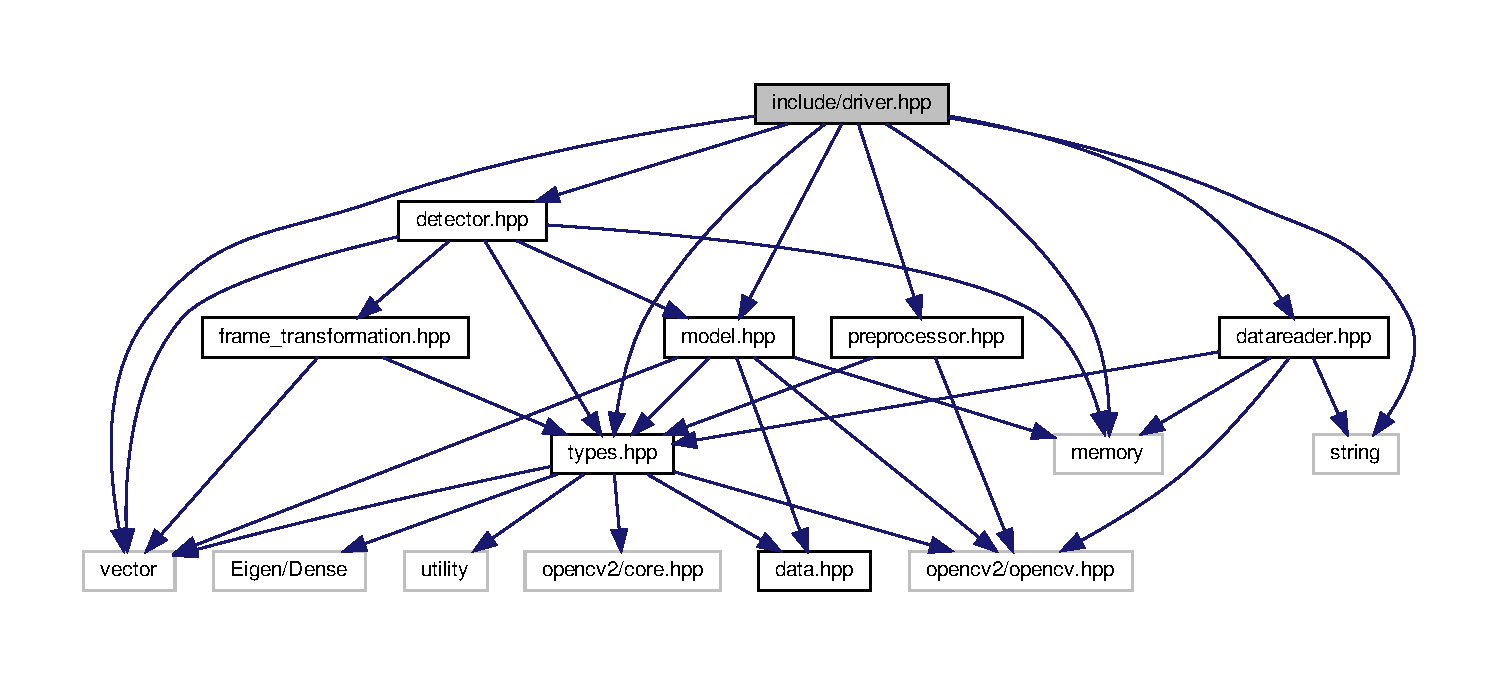
\includegraphics[width=350pt]{driver_8hpp__incl}
\end{center}
\end{figure}
This graph shows which files directly or indirectly include this file\+:
\nopagebreak
\begin{figure}[H]
\begin{center}
\leavevmode
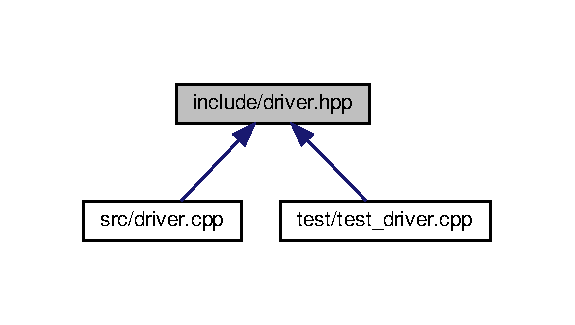
\includegraphics[width=276pt]{driver_8hpp__dep__incl}
\end{center}
\end{figure}
\subsection*{Classes}
\begin{DoxyCompactItemize}
\item 
class \hyperlink{classDriver}{Driver}
\begin{DoxyCompactList}\small\item\em This class is responsible for executing the complete detection pipline. \end{DoxyCompactList}\end{DoxyCompactItemize}


\subsection{Detailed Description}
header file for \hyperlink{driver_8cpp}{driver.\+cpp} 

M\+IT License

Copyright (c) 2021 Anubhav Paras, Sakshi Kakde, Siddharth Telang

Permission is hereby granted, free of charge, to any person obtaining a copy of this software and associated documentation files (the \char`\"{}\+Software\char`\"{}), to deal in the Software without restriction, including without limitation the rights to use, copy, modify, merge, publish, distribute, sublicense, and/or sell copies of the Software, and to permit persons to whom the Software is furnished to do so, subject to the following conditions\+:

The above copyright notice and this permission notice shall be included in all copies or substantial portions of the Software.
\begin{DoxyItemize}
\item T\+HE S\+O\+F\+T\+W\+A\+RE IS P\+R\+O\+V\+I\+D\+ED \char`\"{}\+A\+S I\+S\char`\"{}, W\+I\+T\+H\+O\+UT W\+A\+R\+R\+A\+N\+TY OF A\+NY K\+I\+ND, E\+X\+P\+R\+E\+SS OR I\+M\+P\+L\+I\+ED, I\+N\+C\+L\+U\+D\+I\+NG B\+UT N\+OT L\+I\+M\+I\+T\+ED TO T\+HE W\+A\+R\+R\+A\+N\+T\+I\+ES OF M\+E\+R\+C\+H\+A\+N\+T\+A\+B\+I\+L\+I\+TY, F\+I\+T\+N\+E\+SS F\+OR A P\+A\+R\+T\+I\+C\+U\+L\+AR P\+U\+R\+P\+O\+SE A\+ND N\+O\+N\+I\+N\+F\+R\+I\+N\+G\+E\+M\+E\+NT. IN NO E\+V\+E\+NT S\+H\+A\+LL T\+HE A\+U\+T\+H\+O\+RS OR C\+O\+P\+Y\+R\+I\+G\+HT H\+O\+L\+D\+E\+RS BE L\+I\+A\+B\+LE F\+OR A\+NY C\+L\+A\+IM, D\+A\+M\+A\+G\+ES OR O\+T\+H\+ER L\+I\+A\+B\+I\+L\+I\+TY, W\+H\+E\+T\+H\+ER IN AN A\+C\+T\+I\+ON OF C\+O\+N\+T\+R\+A\+CT, T\+O\+RT OR O\+T\+H\+E\+R\+W\+I\+SE, A\+R\+I\+S\+I\+NG F\+R\+OM, O\+UT OF OR IN C\+O\+N\+N\+E\+C\+T\+I\+ON W\+I\+TH T\+HE S\+O\+F\+T\+W\+A\+RE OR T\+HE U\+SE OR O\+T\+H\+ER D\+E\+A\+L\+I\+N\+GS IN T\+HE S\+O\+F\+T\+W\+A\+RE.
\end{DoxyItemize}

\begin{DoxyAuthor}{Author}
Anubhav Paras (\href{mailto:anubhav@umd.edu}{\tt anubhav@umd.\+edu}) 

Sakshi Kakde (\href{mailto:sakshi@umd.edu}{\tt sakshi@umd.\+edu}) 

Siddharth Telang (\href{mailto:stelang@umd.edu}{\tt stelang@umd.\+edu}) 
\end{DoxyAuthor}
\begin{DoxyVersion}{Version}
0.\+1 
\end{DoxyVersion}
\begin{DoxyDate}{Date}
2021-\/10-\/25
\end{DoxyDate}
\begin{DoxyCopyright}{Copyright}
Copyright (c) 2021 
\end{DoxyCopyright}

\hypertarget{frame__transformation_8hpp}{}\section{include/frame\+\_\+transformation.hpp File Reference}
\label{frame__transformation_8hpp}\index{include/frame\+\_\+transformation.\+hpp@{include/frame\+\_\+transformation.\+hpp}}


header file for \hyperlink{frame__transformation_8cpp}{frame\+\_\+transformation.\+cpp}  


{\ttfamily \#include $<$vector$>$}\newline
{\ttfamily \#include $<$types.\+hpp$>$}\newline
Include dependency graph for frame\+\_\+transformation.\+hpp\+:
\nopagebreak
\begin{figure}[H]
\begin{center}
\leavevmode
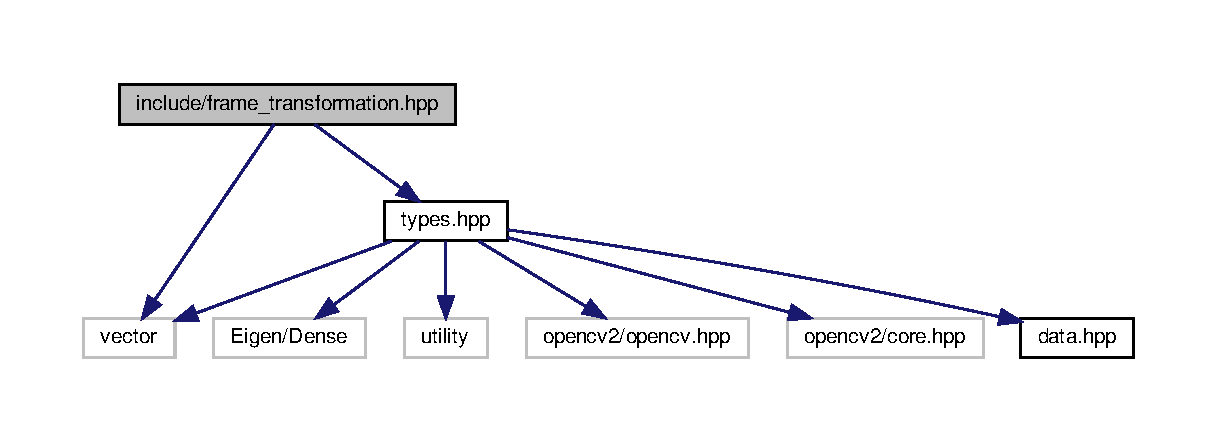
\includegraphics[width=350pt]{frame__transformation_8hpp__incl}
\end{center}
\end{figure}
This graph shows which files directly or indirectly include this file\+:
\nopagebreak
\begin{figure}[H]
\begin{center}
\leavevmode
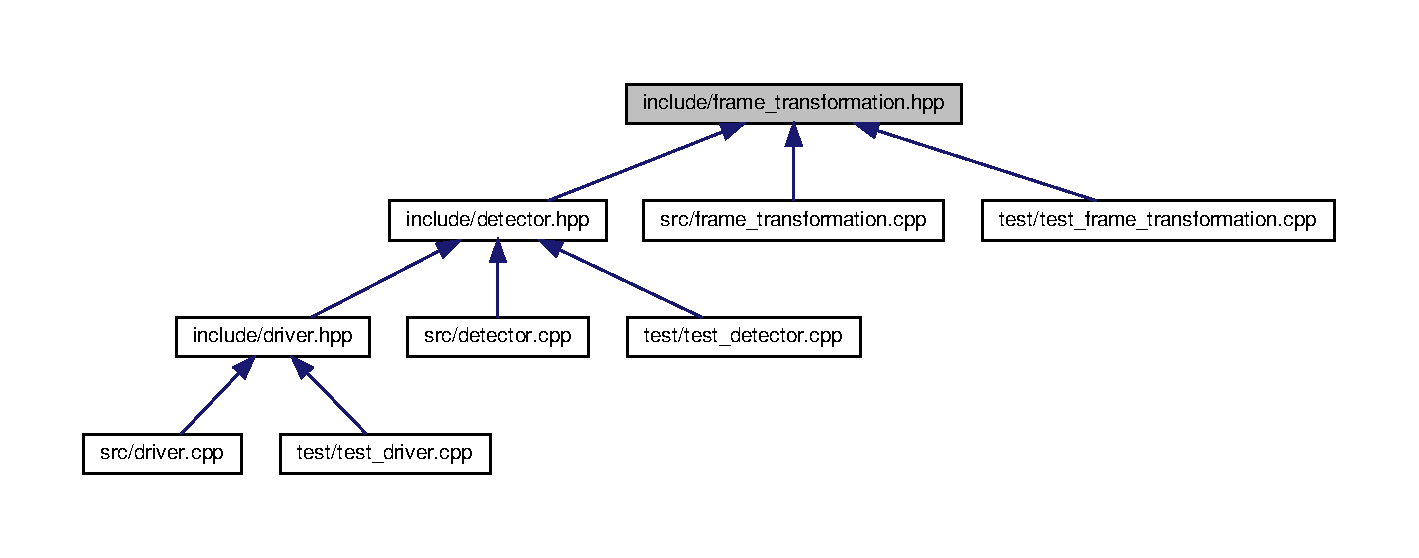
\includegraphics[width=350pt]{frame__transformation_8hpp__dep__incl}
\end{center}
\end{figure}
\subsection*{Classes}
\begin{DoxyCompactItemize}
\item 
class \hyperlink{classFrameTransformation}{Frame\+Transformation}
\begin{DoxyCompactList}\small\item\em Class responsible to convert the coordinates from camera frame to robot frame. \end{DoxyCompactList}\end{DoxyCompactItemize}


\subsection{Detailed Description}
header file for \hyperlink{frame__transformation_8cpp}{frame\+\_\+transformation.\+cpp} 

M\+IT License

Copyright (c) 2021 Anubhav Paras, Sakshi Kakde, Siddharth Telang

Permission is hereby granted, free of charge, to any person obtaining a copy of this software and associated documentation files (the \char`\"{}\+Software\char`\"{}), to deal in the Software without restriction, including without limitation the rights to use, copy, modify, merge, publish, distribute, sublicense, and/or sell copies of the Software, and to permit persons to whom the Software is furnished to do so, subject to the following conditions\+:

The above copyright notice and this permission notice shall be included in all copies or substantial portions of the Software.

T\+HE S\+O\+F\+T\+W\+A\+RE IS P\+R\+O\+V\+I\+D\+ED \char`\"{}\+A\+S I\+S\char`\"{}, W\+I\+T\+H\+O\+UT W\+A\+R\+R\+A\+N\+TY OF A\+NY K\+I\+ND, E\+X\+P\+R\+E\+SS OR I\+M\+P\+L\+I\+ED, I\+N\+C\+L\+U\+D\+I\+NG B\+UT N\+OT L\+I\+M\+I\+T\+ED TO T\+HE W\+A\+R\+R\+A\+N\+T\+I\+ES OF M\+E\+R\+C\+H\+A\+N\+T\+A\+B\+I\+L\+I\+TY, F\+I\+T\+N\+E\+SS F\+OR A P\+A\+R\+T\+I\+C\+U\+L\+AR P\+U\+R\+P\+O\+SE A\+ND N\+O\+N\+I\+N\+F\+R\+I\+N\+G\+E\+M\+E\+NT. IN NO E\+V\+E\+NT S\+H\+A\+LL T\+HE A\+U\+T\+H\+O\+RS OR C\+O\+P\+Y\+R\+I\+G\+HT H\+O\+L\+D\+E\+RS BE L\+I\+A\+B\+LE F\+OR A\+NY C\+L\+A\+IM, D\+A\+M\+A\+G\+ES OR O\+T\+H\+ER L\+I\+A\+B\+I\+L\+I\+TY, W\+H\+E\+T\+H\+ER IN AN A\+C\+T\+I\+ON OF C\+O\+N\+T\+R\+A\+CT, T\+O\+RT OR O\+T\+H\+E\+R\+W\+I\+SE, A\+R\+I\+S\+I\+NG F\+R\+OM, O\+UT OF OR IN C\+O\+N\+N\+E\+C\+T\+I\+ON W\+I\+TH T\+HE S\+O\+F\+T\+W\+A\+RE OR T\+HE U\+SE OR O\+T\+H\+ER D\+E\+A\+L\+I\+N\+GS IN T\+HE S\+O\+F\+T\+W\+A\+RE.

\begin{DoxyAuthor}{Author}
Anubhav Paras (\href{mailto:anubhav@umd.edu}{\tt anubhav@umd.\+edu}) 

Sakshi Kakde (\href{mailto:sakshi@umd.edu}{\tt sakshi@umd.\+edu}) 

Siddharth Telang (\href{mailto:stelang@umd.edu}{\tt stelang@umd.\+edu}) 
\end{DoxyAuthor}
\begin{DoxyVersion}{Version}
0.\+1 
\end{DoxyVersion}
\begin{DoxyDate}{Date}
2021-\/10-\/25
\end{DoxyDate}
\begin{DoxyCopyright}{Copyright}
Copyright (c) 2021 
\end{DoxyCopyright}

\hypertarget{model_8hpp}{}\section{include/model.hpp File Reference}
\label{model_8hpp}\index{include/model.\+hpp@{include/model.\+hpp}}


header file for \hyperlink{model_8cpp}{model.\+cpp}  


{\ttfamily \#include $<$vector$>$}\newline
{\ttfamily \#include $<$memory$>$}\newline
{\ttfamily \#include $<$opencv2/opencv.\+hpp$>$}\newline
{\ttfamily \#include $<$data.\+hpp$>$}\newline
{\ttfamily \#include $<$types.\+hpp$>$}\newline
Include dependency graph for model.\+hpp\+:
\nopagebreak
\begin{figure}[H]
\begin{center}
\leavevmode
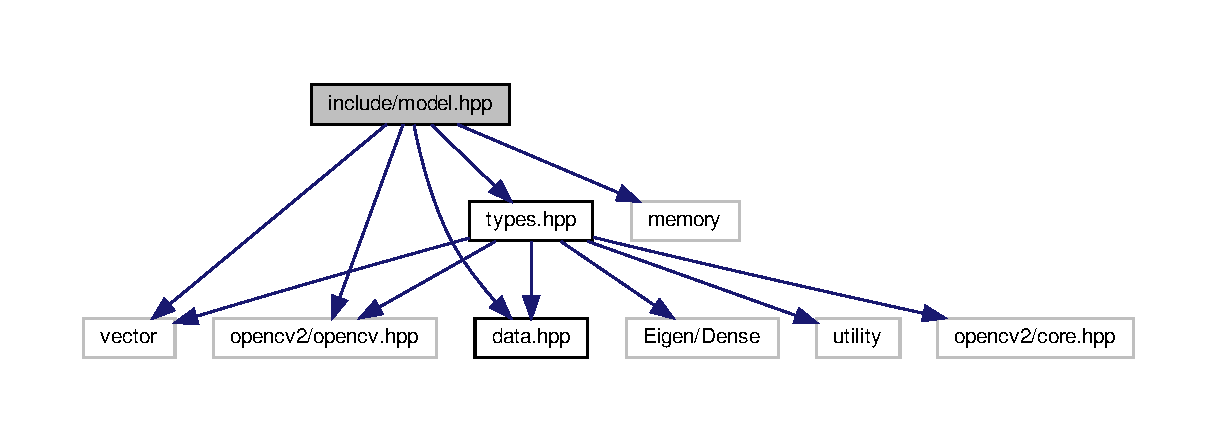
\includegraphics[width=350pt]{model_8hpp__incl}
\end{center}
\end{figure}
This graph shows which files directly or indirectly include this file\+:
\nopagebreak
\begin{figure}[H]
\begin{center}
\leavevmode
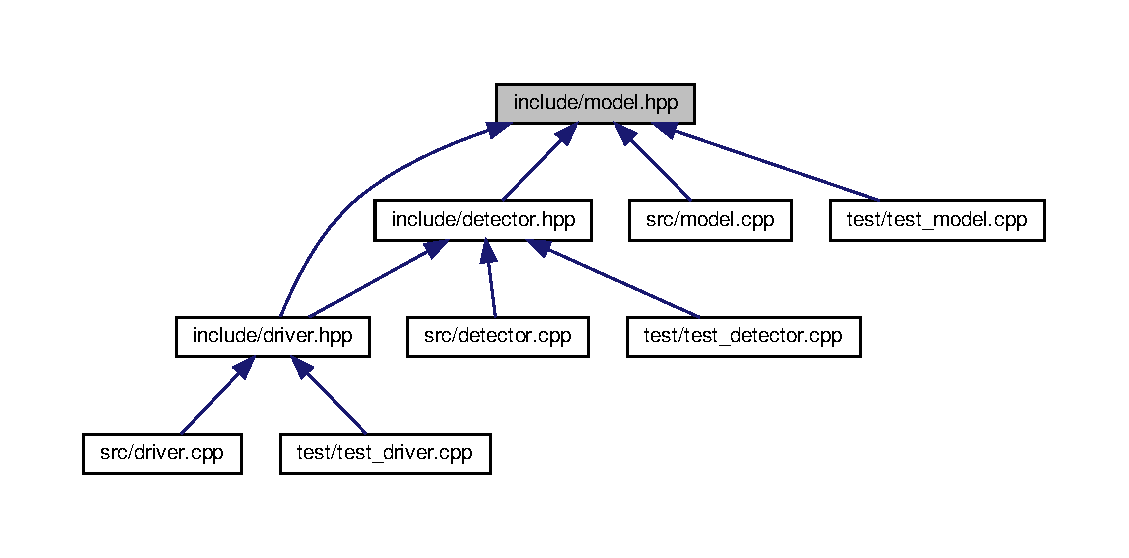
\includegraphics[width=350pt]{model_8hpp__dep__incl}
\end{center}
\end{figure}
\subsection*{Classes}
\begin{DoxyCompactItemize}
\item 
class \hyperlink{classModel}{Model$<$ T, U $>$}
\begin{DoxyCompactList}\small\item\em Abstract \hyperlink{classModel}{Model} class for all the ML models. \end{DoxyCompactList}\item 
class \hyperlink{classSVMHumanClassifier}{S\+V\+M\+Human\+Classifier}
\end{DoxyCompactItemize}


\subsection{Detailed Description}
header file for \hyperlink{model_8cpp}{model.\+cpp} 

M\+IT License

Copyright (c) 2021 Anubhav Paras, Sakshi Kakde, Siddharth Telang

Permission is hereby granted, free of charge, to any person obtaining a copy of this software and associated documentation files (the \char`\"{}\+Software\char`\"{}), to deal in the Software without restriction, including without limitation the rights to use, copy, modify, merge, publish, distribute, sublicense, and/or sell copies of the Software, and to permit persons to whom the Software is furnished to do so, subject to the following conditions\+:

The above copyright notice and this permission notice shall be included in all copies or substantial portions of the Software.

T\+HE S\+O\+F\+T\+W\+A\+RE IS P\+R\+O\+V\+I\+D\+ED \char`\"{}\+A\+S I\+S\char`\"{}, W\+I\+T\+H\+O\+UT W\+A\+R\+R\+A\+N\+TY OF A\+NY K\+I\+ND, E\+X\+P\+R\+E\+SS OR I\+M\+P\+L\+I\+ED, I\+N\+C\+L\+U\+D\+I\+NG B\+UT N\+OT L\+I\+M\+I\+T\+ED TO T\+HE W\+A\+R\+R\+A\+N\+T\+I\+ES OF M\+E\+R\+C\+H\+A\+N\+T\+A\+B\+I\+L\+I\+TY, F\+I\+T\+N\+E\+SS F\+OR A P\+A\+R\+T\+I\+C\+U\+L\+AR P\+U\+R\+P\+O\+SE A\+ND N\+O\+N\+I\+N\+F\+R\+I\+N\+G\+E\+M\+E\+NT. IN NO E\+V\+E\+NT S\+H\+A\+LL T\+HE A\+U\+T\+H\+O\+RS OR C\+O\+P\+Y\+R\+I\+G\+HT H\+O\+L\+D\+E\+RS BE L\+I\+A\+B\+LE F\+OR A\+NY C\+L\+A\+IM, D\+A\+M\+A\+G\+ES OR O\+T\+H\+ER L\+I\+A\+B\+I\+L\+I\+TY, W\+H\+E\+T\+H\+ER IN AN A\+C\+T\+I\+ON OF C\+O\+N\+T\+R\+A\+CT, T\+O\+RT OR O\+T\+H\+E\+R\+W\+I\+SE, A\+R\+I\+S\+I\+NG F\+R\+OM, O\+UT OF OR IN C\+O\+N\+N\+E\+C\+T\+I\+ON W\+I\+TH T\+HE S\+O\+F\+T\+W\+A\+RE OR T\+HE U\+SE OR O\+T\+H\+ER D\+E\+A\+L\+I\+N\+GS IN T\+HE S\+O\+F\+T\+W\+A\+RE.

\begin{DoxyAuthor}{Author}
Anubhav Paras (\href{mailto:anubhav@umd.edu}{\tt anubhav@umd.\+edu}) 

Sakshi Kakde (\href{mailto:sakshi@umd.edu}{\tt sakshi@umd.\+edu}) 

Siddharth Telang (\href{mailto:stelang@umd.edu}{\tt stelang@umd.\+edu}) 
\end{DoxyAuthor}
\begin{DoxyVersion}{Version}
0.\+1 
\end{DoxyVersion}
\begin{DoxyDate}{Date}
2021-\/10-\/25
\end{DoxyDate}
\begin{DoxyCopyright}{Copyright}
Copyright (c) 2021 
\end{DoxyCopyright}

\hypertarget{preprocessor_8hpp}{}\section{include/preprocessor.hpp File Reference}
\label{preprocessor_8hpp}\index{include/preprocessor.\+hpp@{include/preprocessor.\+hpp}}


header file for \hyperlink{preprocessor_8cpp}{preprocessor.\+cpp}  


{\ttfamily \#include $<$opencv2/opencv.\+hpp$>$}\newline
{\ttfamily \#include $<$types.\+hpp$>$}\newline
Include dependency graph for preprocessor.\+hpp\+:
\nopagebreak
\begin{figure}[H]
\begin{center}
\leavevmode
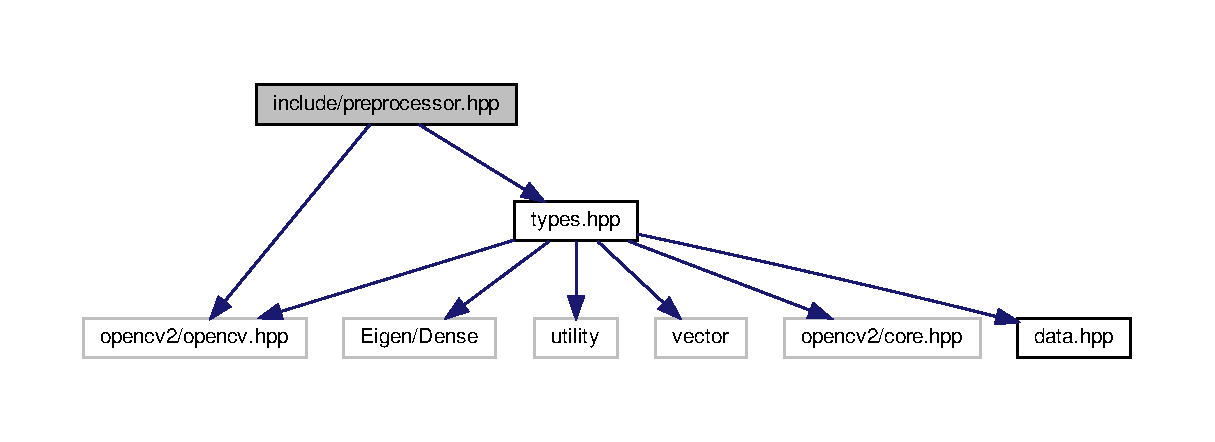
\includegraphics[width=350pt]{preprocessor_8hpp__incl}
\end{center}
\end{figure}
This graph shows which files directly or indirectly include this file\+:
\nopagebreak
\begin{figure}[H]
\begin{center}
\leavevmode
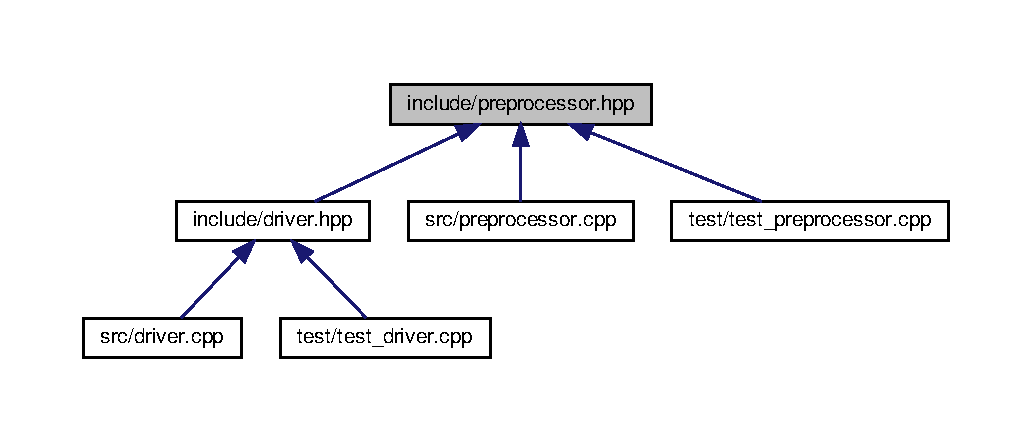
\includegraphics[width=350pt]{preprocessor_8hpp__dep__incl}
\end{center}
\end{figure}
\subsection*{Classes}
\begin{DoxyCompactItemize}
\item 
class \hyperlink{classPreProcessor}{Pre\+Processor}
\begin{DoxyCompactList}\small\item\em Class to do all the preprocessing of the data. \end{DoxyCompactList}\end{DoxyCompactItemize}


\subsection{Detailed Description}
header file for \hyperlink{preprocessor_8cpp}{preprocessor.\+cpp} 

M\+IT License

Copyright (c) 2021 Anubhav Paras, Sakshi Kakde, Siddharth Telang

Permission is hereby granted, free of charge, to any person obtaining a copy of this software and associated documentation files (the \char`\"{}\+Software\char`\"{}), to deal in the Software without restriction, including without limitation the rights to use, copy, modify, merge, publish, distribute, sublicense, and/or sell copies of the Software, and to permit persons to whom the Software is furnished to do so, subject to the following conditions\+:

The above copyright notice and this permission notice shall be included in all copies or substantial portions of the Software.

T\+HE S\+O\+F\+T\+W\+A\+RE IS P\+R\+O\+V\+I\+D\+ED \char`\"{}\+A\+S I\+S\char`\"{}, W\+I\+T\+H\+O\+UT W\+A\+R\+R\+A\+N\+TY OF A\+NY K\+I\+ND, E\+X\+P\+R\+E\+SS OR I\+M\+P\+L\+I\+ED, I\+N\+C\+L\+U\+D\+I\+NG B\+UT N\+OT L\+I\+M\+I\+T\+ED TO T\+HE W\+A\+R\+R\+A\+N\+T\+I\+ES OF M\+E\+R\+C\+H\+A\+N\+T\+A\+B\+I\+L\+I\+TY, F\+I\+T\+N\+E\+SS F\+OR A P\+A\+R\+T\+I\+C\+U\+L\+AR P\+U\+R\+P\+O\+SE A\+ND N\+O\+N\+I\+N\+F\+R\+I\+N\+G\+E\+M\+E\+NT. IN NO E\+V\+E\+NT S\+H\+A\+LL T\+HE A\+U\+T\+H\+O\+RS OR C\+O\+P\+Y\+R\+I\+G\+HT H\+O\+L\+D\+E\+RS BE L\+I\+A\+B\+LE F\+OR A\+NY C\+L\+A\+IM, D\+A\+M\+A\+G\+ES OR O\+T\+H\+ER L\+I\+A\+B\+I\+L\+I\+TY, W\+H\+E\+T\+H\+ER IN AN A\+C\+T\+I\+ON OF C\+O\+N\+T\+R\+A\+CT, T\+O\+RT OR O\+T\+H\+E\+R\+W\+I\+SE, A\+R\+I\+S\+I\+NG F\+R\+OM, O\+UT OF OR IN C\+O\+N\+N\+E\+C\+T\+I\+ON W\+I\+TH T\+HE S\+O\+F\+T\+W\+A\+RE OR T\+HE U\+SE OR O\+T\+H\+ER D\+E\+A\+L\+I\+N\+GS IN T\+HE S\+O\+F\+T\+W\+A\+RE.

\begin{DoxyAuthor}{Author}
Anubhav Paras (\href{mailto:anubhav@umd.edu}{\tt anubhav@umd.\+edu}) 

Sakshi Kakde (\href{mailto:sakshi@umd.edu}{\tt sakshi@umd.\+edu}) 

Siddharth Telang (\href{mailto:stelang@umd.edu}{\tt stelang@umd.\+edu}) 
\end{DoxyAuthor}
\begin{DoxyVersion}{Version}
0.\+1 
\end{DoxyVersion}
\begin{DoxyDate}{Date}
2021-\/10-\/25
\end{DoxyDate}
\begin{DoxyCopyright}{Copyright}
Copyright (c) 2021 
\end{DoxyCopyright}

\hypertarget{types_8hpp}{}\section{include/types.hpp File Reference}
\label{types_8hpp}\index{include/types.\+hpp@{include/types.\+hpp}}


contains various typedefs  


{\ttfamily \#include $<$Eigen/\+Dense$>$}\newline
{\ttfamily \#include $<$utility$>$}\newline
{\ttfamily \#include $<$vector$>$}\newline
{\ttfamily \#include $<$opencv2/opencv.\+hpp$>$}\newline
{\ttfamily \#include $<$opencv2/core.\+hpp$>$}\newline
{\ttfamily \#include $<$data.\+hpp$>$}\newline
Include dependency graph for types.\+hpp\+:
\nopagebreak
\begin{figure}[H]
\begin{center}
\leavevmode
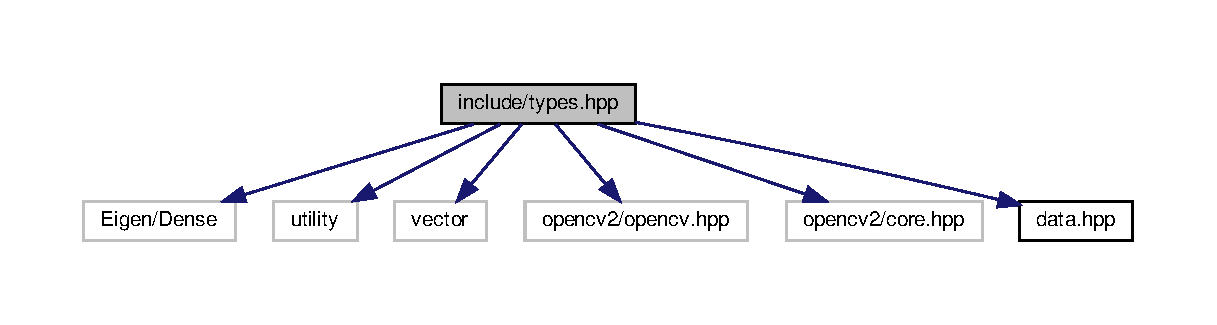
\includegraphics[width=350pt]{types_8hpp__incl}
\end{center}
\end{figure}
This graph shows which files directly or indirectly include this file\+:
\nopagebreak
\begin{figure}[H]
\begin{center}
\leavevmode
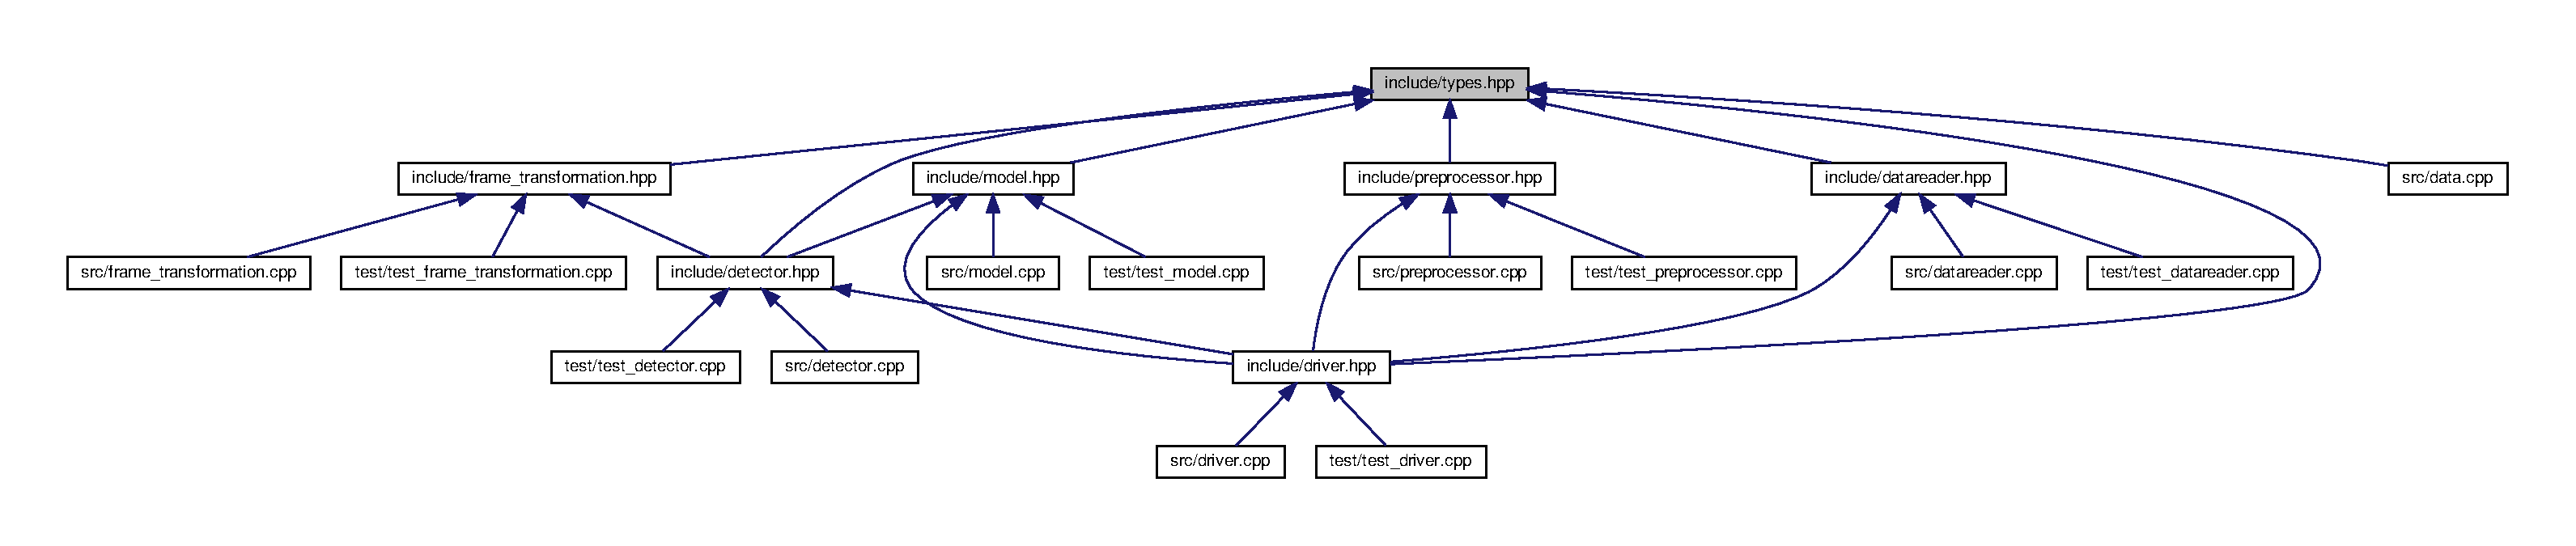
\includegraphics[width=350pt]{types_8hpp__dep__incl}
\end{center}
\end{figure}
\subsection*{Classes}
\begin{DoxyCompactItemize}
\item 
struct \hyperlink{structCentroid}{Centroid}
\end{DoxyCompactItemize}
\subsection*{Typedefs}
\begin{DoxyCompactItemize}
\item 
\mbox{\Hypertarget{types_8hpp_a7edea8e3b5fb20fbd4527baf12ffb97a}\label{types_8hpp_a7edea8e3b5fb20fbd4527baf12ffb97a}} 
typedef std\+::vector$<$ cv\+::\+Rect $>$ {\bfseries Rectangles}
\item 
\mbox{\Hypertarget{types_8hpp_ab47b2f4d68521bc90d778ddf94c51585}\label{types_8hpp_ab47b2f4d68521bc90d778ddf94c51585}} 
typedef cv\+::\+Input\+Array {\bfseries Image}
\item 
\mbox{\Hypertarget{types_8hpp_a9fd4abfb6a16669ad825115ef21fa4ca}\label{types_8hpp_a9fd4abfb6a16669ad825115ef21fa4ca}} 
typedef cv\+::\+H\+O\+G\+Descriptor {\bfseries S\+V\+M\+H\+O\+G\+Model}
\item 
\mbox{\Hypertarget{types_8hpp_adfeac77ddc14cd16fa7f6cd1821a3b87}\label{types_8hpp_adfeac77ddc14cd16fa7f6cd1821a3b87}} 
typedef std\+::pair$<$ Rectangles, std\+::vector$<$ double $>$ $>$ {\bfseries Rectangles\+And\+Scores}
\item 
\mbox{\Hypertarget{types_8hpp_a5199bad41e470890301f3d228a67eac5}\label{types_8hpp_a5199bad41e470890301f3d228a67eac5}} 
typedef \hyperlink{classData}{Data}$<$ Rectangles\+And\+Scores $>$ {\bfseries Detection\+Output}
\item 
\mbox{\Hypertarget{types_8hpp_a959d2ba5f833ae4cd440bd2bf543c83f}\label{types_8hpp_a959d2ba5f833ae4cd440bd2bf543c83f}} 
typedef cv\+::\+Point3d {\bfseries Coord3D}
\item 
\mbox{\Hypertarget{types_8hpp_a8e82e2f9fcd848a3484f1d44124e10ee}\label{types_8hpp_a8e82e2f9fcd848a3484f1d44124e10ee}} 
typedef cv\+::\+Point {\bfseries Coord2D}
\item 
\mbox{\Hypertarget{types_8hpp_abfb1ae9cce37137365824ec13c2f6dff}\label{types_8hpp_abfb1ae9cce37137365824ec13c2f6dff}} 
typedef struct \hyperlink{structCentroid}{Centroid} {\bfseries Centroid}
\end{DoxyCompactItemize}


\subsection{Detailed Description}
contains various typedefs 

M\+IT License

Copyright (c) 2021 Anubhav Paras, Sakshi Kakde, Siddharth Telang

Permission is hereby granted, free of charge, to any person obtaining a copy of this software and associated documentation files (the \char`\"{}\+Software\char`\"{}), to deal in the Software without restriction, including without limitation the rights to use, copy, modify, merge, publish, distribute, sublicense, and/or sell copies of the Software, and to permit persons to whom the Software is furnished to do so, subject to the following conditions\+:

The above copyright notice and this permission notice shall be included in all copies or substantial portions of the Software.

T\+HE S\+O\+F\+T\+W\+A\+RE IS P\+R\+O\+V\+I\+D\+ED \char`\"{}\+A\+S I\+S\char`\"{}, W\+I\+T\+H\+O\+UT W\+A\+R\+R\+A\+N\+TY OF A\+NY K\+I\+ND, E\+X\+P\+R\+E\+SS OR I\+M\+P\+L\+I\+ED, I\+N\+C\+L\+U\+D\+I\+NG B\+UT N\+OT L\+I\+M\+I\+T\+ED TO T\+HE W\+A\+R\+R\+A\+N\+T\+I\+ES OF M\+E\+R\+C\+H\+A\+N\+T\+A\+B\+I\+L\+I\+TY, F\+I\+T\+N\+E\+SS F\+OR A P\+A\+R\+T\+I\+C\+U\+L\+AR P\+U\+R\+P\+O\+SE A\+ND N\+O\+N\+I\+N\+F\+R\+I\+N\+G\+E\+M\+E\+NT. IN NO E\+V\+E\+NT S\+H\+A\+LL T\+HE A\+U\+T\+H\+O\+RS OR C\+O\+P\+Y\+R\+I\+G\+HT H\+O\+L\+D\+E\+RS BE L\+I\+A\+B\+LE F\+OR A\+NY C\+L\+A\+IM, D\+A\+M\+A\+G\+ES OR O\+T\+H\+ER L\+I\+A\+B\+I\+L\+I\+TY, W\+H\+E\+T\+H\+ER IN AN A\+C\+T\+I\+ON OF C\+O\+N\+T\+R\+A\+CT, T\+O\+RT OR O\+T\+H\+E\+R\+W\+I\+SE, A\+R\+I\+S\+I\+NG F\+R\+OM, O\+UT OF OR IN C\+O\+N\+N\+E\+C\+T\+I\+ON W\+I\+TH T\+HE S\+O\+F\+T\+W\+A\+RE OR T\+HE U\+SE OR O\+T\+H\+ER D\+E\+A\+L\+I\+N\+GS IN T\+HE S\+O\+F\+T\+W\+A\+RE.

\begin{DoxyAuthor}{Author}
Anubhav Paras (\href{mailto:anubhav@umd.edu}{\tt anubhav@umd.\+edu}) 

Sakshi Kakde (\href{mailto:sakshi@umd.edu}{\tt sakshi@umd.\+edu}) 

Siddharth Telang (\href{mailto:stelang@umd.edu}{\tt stelang@umd.\+edu}) 
\end{DoxyAuthor}
\begin{DoxyVersion}{Version}
0.\+1 
\end{DoxyVersion}
\begin{DoxyDate}{Date}
2021-\/10-\/25
\end{DoxyDate}
\begin{DoxyCopyright}{Copyright}
Copyright (c) 2021 
\end{DoxyCopyright}

\hypertarget{data_8cpp}{}\section{src/data.cpp File Reference}
\label{data_8cpp}\index{src/data.\+cpp@{src/data.\+cpp}}


\hyperlink{classData}{Data} class template.  


{\ttfamily \#include $<$data.\+hpp$>$}\newline
{\ttfamily \#include $<$type\+\_\+traits$>$}\newline
{\ttfamily \#include $<$types.\+hpp$>$}\newline
Include dependency graph for data.\+cpp\+:
\nopagebreak
\begin{figure}[H]
\begin{center}
\leavevmode
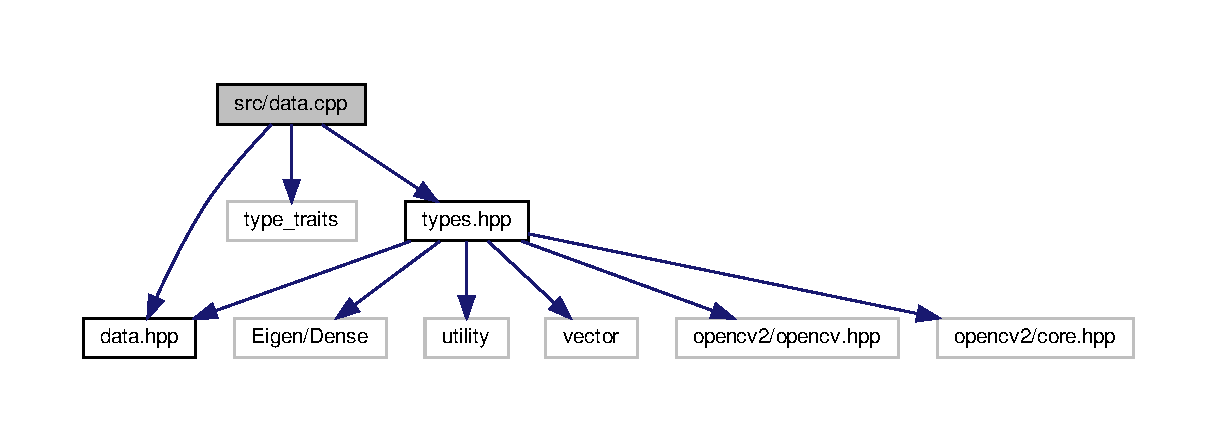
\includegraphics[width=350pt]{data_8cpp__incl}
\end{center}
\end{figure}


\subsection{Detailed Description}
\hyperlink{classData}{Data} class template. 

M\+IT License

Copyright (c) 2021 Anubhav Paras, Sakshi Kakde, Siddharth Telang

Permission is hereby granted, free of charge, to any person obtaining a copy of this software and associated documentation files (the \char`\"{}\+Software\char`\"{}), to deal in the Software without restriction, including without limitation the rights to use, copy, modify, merge, publish, distribute, sublicense, and/or sell copies of the Software, and to permit persons to whom the Software is furnished to do so, subject to the following conditions\+:

The above copyright notice and this permission notice shall be included in all copies or substantial portions of the Software.

T\+HE S\+O\+F\+T\+W\+A\+RE IS P\+R\+O\+V\+I\+D\+ED \char`\"{}\+A\+S I\+S\char`\"{}, W\+I\+T\+H\+O\+UT W\+A\+R\+R\+A\+N\+TY OF A\+NY K\+I\+ND, E\+X\+P\+R\+E\+SS OR I\+M\+P\+L\+I\+ED, I\+N\+C\+L\+U\+D\+I\+NG B\+UT N\+OT L\+I\+M\+I\+T\+ED TO T\+HE W\+A\+R\+R\+A\+N\+T\+I\+ES OF M\+E\+R\+C\+H\+A\+N\+T\+A\+B\+I\+L\+I\+TY, F\+I\+T\+N\+E\+SS F\+OR A P\+A\+R\+T\+I\+C\+U\+L\+AR P\+U\+R\+P\+O\+SE A\+ND N\+O\+N\+I\+N\+F\+R\+I\+N\+G\+E\+M\+E\+NT. IN NO E\+V\+E\+NT S\+H\+A\+LL T\+HE A\+U\+T\+H\+O\+RS OR C\+O\+P\+Y\+R\+I\+G\+HT H\+O\+L\+D\+E\+RS BE L\+I\+A\+B\+LE F\+OR A\+NY C\+L\+A\+IM, D\+A\+M\+A\+G\+ES OR O\+T\+H\+ER L\+I\+A\+B\+I\+L\+I\+TY, W\+H\+E\+T\+H\+ER IN AN A\+C\+T\+I\+ON OF C\+O\+N\+T\+R\+A\+CT, T\+O\+RT OR O\+T\+H\+E\+R\+W\+I\+SE, A\+R\+I\+S\+I\+NG F\+R\+OM, O\+UT OF OR IN C\+O\+N\+N\+E\+C\+T\+I\+ON W\+I\+TH T\+HE S\+O\+F\+T\+W\+A\+RE OR T\+HE U\+SE OR O\+T\+H\+ER D\+E\+A\+L\+I\+N\+GS IN T\+HE S\+O\+F\+T\+W\+A\+RE.

\begin{DoxyAuthor}{Author}
Anubhav Paras (\href{mailto:anubhav@umd.edu}{\tt anubhav@umd.\+edu}) 

Sakshi Kakde (\href{mailto:sakshi@umd.edu}{\tt sakshi@umd.\+edu}) 

Siddharth Telang (\href{mailto:stelang@umd.edu}{\tt stelang@umd.\+edu}) 
\end{DoxyAuthor}
\begin{DoxyVersion}{Version}
0.\+1 
\end{DoxyVersion}
\begin{DoxyDate}{Date}
2021-\/10-\/25
\end{DoxyDate}
\begin{DoxyCopyright}{Copyright}
Copyright (c) 2021 
\end{DoxyCopyright}

\hypertarget{datareader_8cpp}{}\section{src/datareader.cpp File Reference}
\label{datareader_8cpp}\index{src/datareader.\+cpp@{src/datareader.\+cpp}}


\hyperlink{classData}{Data} reader file to read the data.  


{\ttfamily \#include $<$datareader.\+hpp$>$}\newline
Include dependency graph for datareader.\+cpp\+:
\nopagebreak
\begin{figure}[H]
\begin{center}
\leavevmode
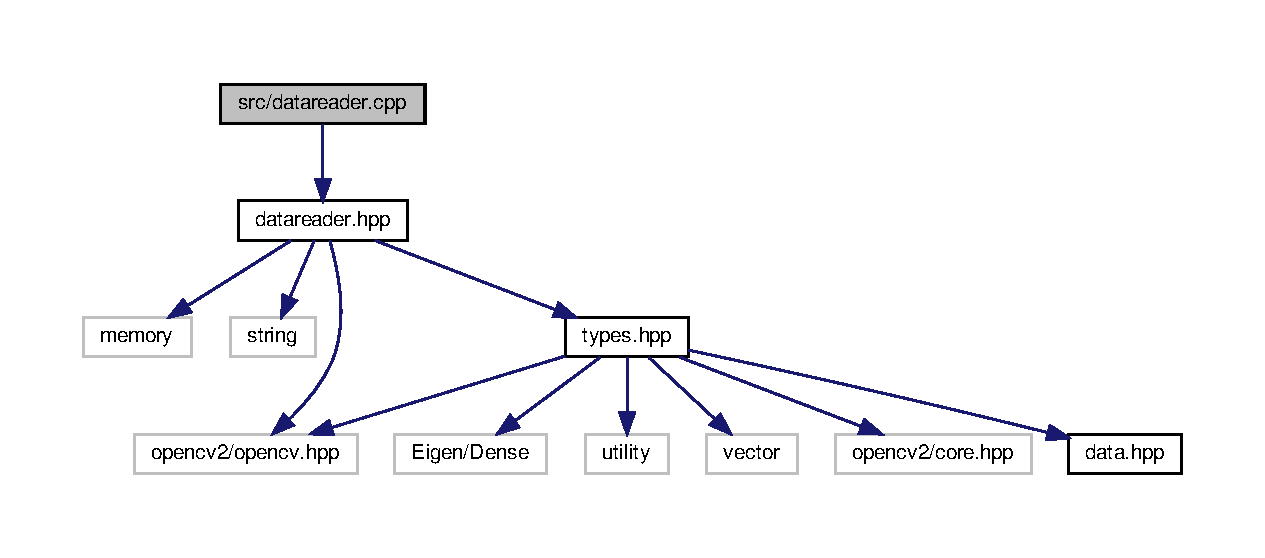
\includegraphics[width=350pt]{datareader_8cpp__incl}
\end{center}
\end{figure}


\subsection{Detailed Description}
\hyperlink{classData}{Data} reader file to read the data. 

M\+IT License

Copyright (c) 2021 Anubhav Paras, Sakshi Kakde, Siddharth Telang

Permission is hereby granted, free of charge, to any person obtaining a copy of this software and associated documentation files (the \char`\"{}\+Software\char`\"{}), to deal in the Software without restriction, including without limitation the rights to use, copy, modify, merge, publish, distribute, sublicense, and/or sell copies of the Software, and to permit persons to whom the Software is furnished to do so, subject to the following conditions\+:

The above copyright notice and this permission notice shall be included in all copies or substantial portions of the Software.

T\+HE S\+O\+F\+T\+W\+A\+RE IS P\+R\+O\+V\+I\+D\+ED \char`\"{}\+A\+S I\+S\char`\"{}, W\+I\+T\+H\+O\+UT W\+A\+R\+R\+A\+N\+TY OF A\+NY K\+I\+ND, E\+X\+P\+R\+E\+SS OR I\+M\+P\+L\+I\+ED, I\+N\+C\+L\+U\+D\+I\+NG B\+UT N\+OT L\+I\+M\+I\+T\+ED TO T\+HE W\+A\+R\+R\+A\+N\+T\+I\+ES OF M\+E\+R\+C\+H\+A\+N\+T\+A\+B\+I\+L\+I\+TY, F\+I\+T\+N\+E\+SS F\+OR A P\+A\+R\+T\+I\+C\+U\+L\+AR P\+U\+R\+P\+O\+SE A\+ND N\+O\+N\+I\+N\+F\+R\+I\+N\+G\+E\+M\+E\+NT. IN NO E\+V\+E\+NT S\+H\+A\+LL T\+HE A\+U\+T\+H\+O\+RS OR C\+O\+P\+Y\+R\+I\+G\+HT H\+O\+L\+D\+E\+RS BE L\+I\+A\+B\+LE F\+OR A\+NY C\+L\+A\+IM, D\+A\+M\+A\+G\+ES OR O\+T\+H\+ER L\+I\+A\+B\+I\+L\+I\+TY, W\+H\+E\+T\+H\+ER IN AN A\+C\+T\+I\+ON OF C\+O\+N\+T\+R\+A\+CT, T\+O\+RT OR O\+T\+H\+E\+R\+W\+I\+SE, A\+R\+I\+S\+I\+NG F\+R\+OM, O\+UT OF OR IN C\+O\+N\+N\+E\+C\+T\+I\+ON W\+I\+TH T\+HE S\+O\+F\+T\+W\+A\+RE OR T\+HE U\+SE OR O\+T\+H\+ER D\+E\+A\+L\+I\+N\+GS IN T\+HE S\+O\+F\+T\+W\+A\+RE.

\begin{DoxyAuthor}{Author}
Anubhav Paras (\href{mailto:anubhav@umd.edu}{\tt anubhav@umd.\+edu}) 

Sakshi Kakde (\href{mailto:sakshi@umd.edu}{\tt sakshi@umd.\+edu}) 

Siddharth Telang (\href{mailto:stelang@umd.edu}{\tt stelang@umd.\+edu}) 
\end{DoxyAuthor}
\begin{DoxyVersion}{Version}
0.\+1 
\end{DoxyVersion}
\begin{DoxyDate}{Date}
2021-\/10-\/25
\end{DoxyDate}
\begin{DoxyCopyright}{Copyright}
Copyright (c) 2021 
\end{DoxyCopyright}

\hypertarget{detector_8cpp}{}\section{src/detector.cpp File Reference}
\label{detector_8cpp}\index{src/detector.\+cpp@{src/detector.\+cpp}}


Implementation of \hyperlink{classDetector}{Detector} class.  


{\ttfamily \#include $<$detector.\+hpp$>$}\newline
{\ttfamily \#include $<$memory$>$}\newline
{\ttfamily \#include $<$unordered\+\_\+map$>$}\newline
{\ttfamily \#include $<$iostream$>$}\newline
{\ttfamily \#include $<$limits$>$}\newline
{\ttfamily \#include $<$string$>$}\newline
{\ttfamily \#include $<$opencv2/opencv.\+hpp$>$}\newline
Include dependency graph for detector.\+cpp\+:
\nopagebreak
\begin{figure}[H]
\begin{center}
\leavevmode
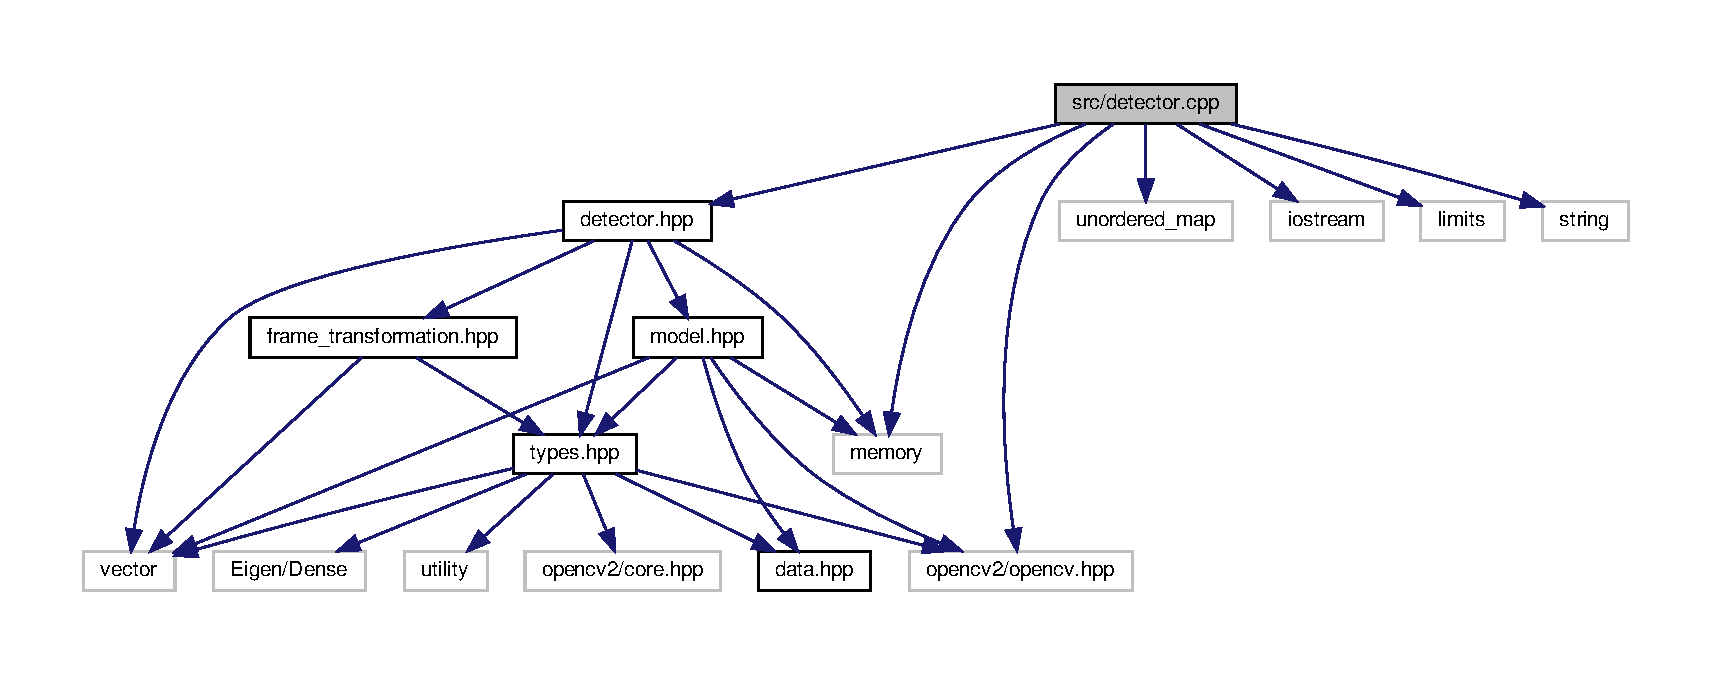
\includegraphics[width=350pt]{detector_8cpp__incl}
\end{center}
\end{figure}
\subsection*{Typedefs}
\begin{DoxyCompactItemize}
\item 
\mbox{\Hypertarget{detector_8cpp_a87e5163fc0ce853fcc53bf43fef27a1a}\label{detector_8cpp_a87e5163fc0ce853fcc53bf43fef27a1a}} 
typedef \hyperlink{classHumanDetector}{Human\+Detector} {\bfseries HD}
\end{DoxyCompactItemize}


\subsection{Detailed Description}
Implementation of \hyperlink{classDetector}{Detector} class. 

M\+IT License

Copyright (c) 2021 Anubhav Paras, Sakshi Kakde, Siddharth Telang

Permission is hereby granted, free of charge, to any person obtaining a copy of this software and associated documentation files (the \char`\"{}\+Software\char`\"{}), to deal in the Software without restriction, including without limitation the rights to use, copy, modify, merge, publish, distribute, sublicense, and/or sell copies of the Software, and to permit persons to whom the Software is furnished to do so, subject to the following conditions\+:

The above copyright notice and this permission notice shall be included in all copies or substantial portions of the Software.

T\+HE S\+O\+F\+T\+W\+A\+RE IS P\+R\+O\+V\+I\+D\+ED \char`\"{}\+A\+S I\+S\char`\"{}, W\+I\+T\+H\+O\+UT W\+A\+R\+R\+A\+N\+TY OF A\+NY K\+I\+ND, E\+X\+P\+R\+E\+SS OR I\+M\+P\+L\+I\+ED, I\+N\+C\+L\+U\+D\+I\+NG B\+UT N\+OT L\+I\+M\+I\+T\+ED TO T\+HE W\+A\+R\+R\+A\+N\+T\+I\+ES OF M\+E\+R\+C\+H\+A\+N\+T\+A\+B\+I\+L\+I\+TY, F\+I\+T\+N\+E\+SS F\+OR A P\+A\+R\+T\+I\+C\+U\+L\+AR P\+U\+R\+P\+O\+SE A\+ND N\+O\+N\+I\+N\+F\+R\+I\+N\+G\+E\+M\+E\+NT. IN NO E\+V\+E\+NT S\+H\+A\+LL T\+HE A\+U\+T\+H\+O\+RS OR C\+O\+P\+Y\+R\+I\+G\+HT H\+O\+L\+D\+E\+RS BE L\+I\+A\+B\+LE F\+OR A\+NY C\+L\+A\+IM, D\+A\+M\+A\+G\+ES OR O\+T\+H\+ER L\+I\+A\+B\+I\+L\+I\+TY, W\+H\+E\+T\+H\+ER IN AN A\+C\+T\+I\+ON OF C\+O\+N\+T\+R\+A\+CT, T\+O\+RT OR O\+T\+H\+E\+R\+W\+I\+SE, A\+R\+I\+S\+I\+NG F\+R\+OM, O\+UT OF OR IN C\+O\+N\+N\+E\+C\+T\+I\+ON W\+I\+TH T\+HE S\+O\+F\+T\+W\+A\+RE OR T\+HE U\+SE OR O\+T\+H\+ER D\+E\+A\+L\+I\+N\+GS IN T\+HE S\+O\+F\+T\+W\+A\+RE.

\begin{DoxyAuthor}{Author}
Anubhav Paras (\href{mailto:anubhav@umd.edu}{\tt anubhav@umd.\+edu}) 

Sakshi Kakde (\href{mailto:sakshi@umd.edu}{\tt sakshi@umd.\+edu}) 

Siddharth Telang (\href{mailto:stelang@umd.edu}{\tt stelang@umd.\+edu}) 
\end{DoxyAuthor}
\begin{DoxyVersion}{Version}
0.\+1 
\end{DoxyVersion}
\begin{DoxyDate}{Date}
2021-\/10-\/25
\end{DoxyDate}
\begin{DoxyCopyright}{Copyright}
Copyright (c) 2021 
\end{DoxyCopyright}

\hypertarget{driver_8cpp}{}\section{src/driver.cpp File Reference}
\label{driver_8cpp}\index{src/driver.\+cpp@{src/driver.\+cpp}}


\hyperlink{classDriver}{Driver} file to execute the main pipeline.  


{\ttfamily \#include $<$driver.\+hpp$>$}\newline
{\ttfamily \#include $<$fstream$>$}\newline
Include dependency graph for driver.\+cpp\+:
\nopagebreak
\begin{figure}[H]
\begin{center}
\leavevmode
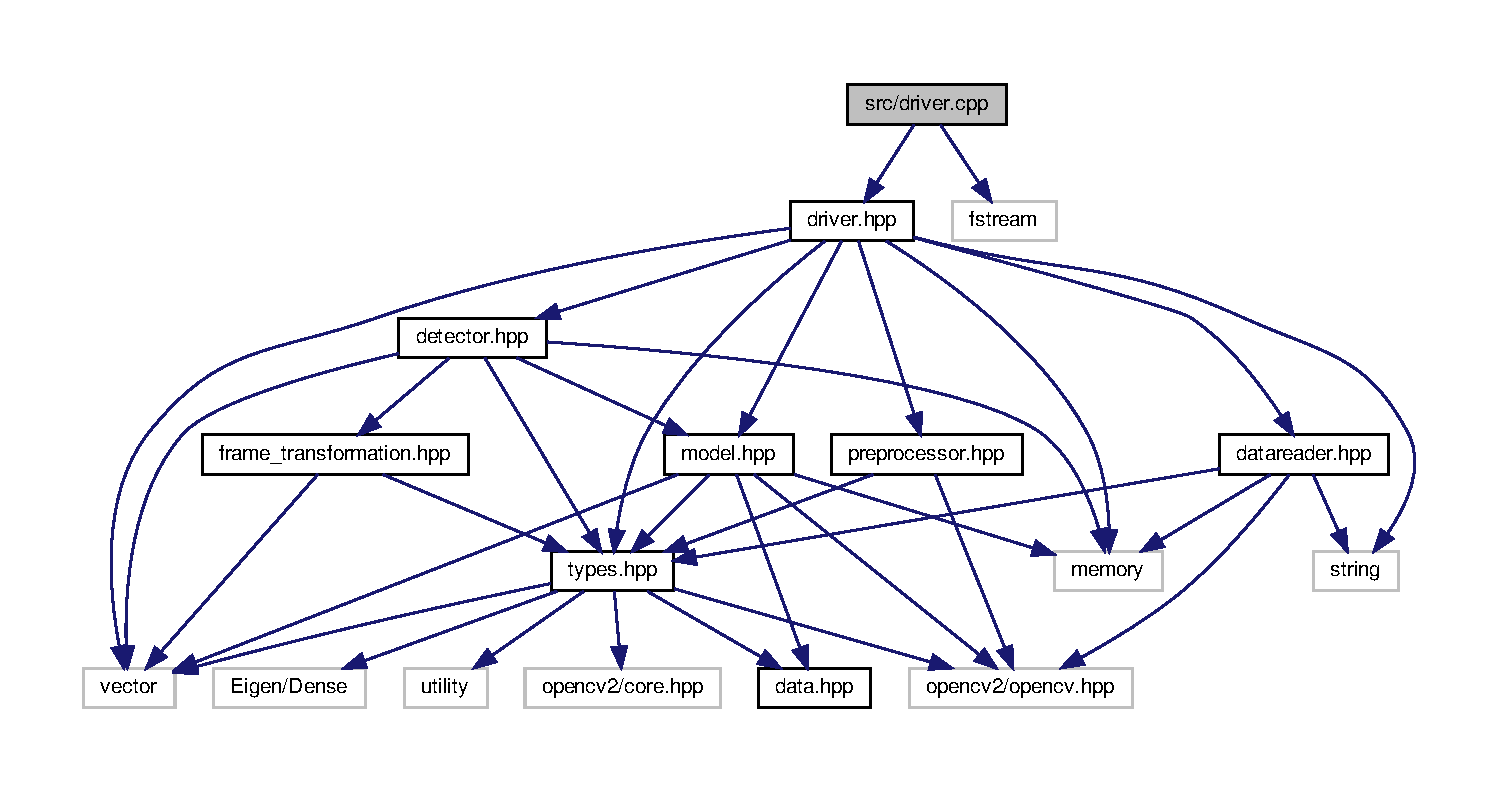
\includegraphics[width=350pt]{driver_8cpp__incl}
\end{center}
\end{figure}


\subsection{Detailed Description}
\hyperlink{classDriver}{Driver} file to execute the main pipeline. 

M\+IT License

Copyright (c) 2021 Anubhav Paras, Sakshi Kakde, Siddharth Telang

Permission is hereby granted, free of charge, to any person obtaining a copy of this software and associated documentation files (the \char`\"{}\+Software\char`\"{}), to deal in the Software without restriction, including without limitation the rights to use, copy, modify, merge, publish, distribute, sublicense, and/or sell copies of the Software, and to permit persons to whom the Software is furnished to do so, subject to the following conditions\+:

The above copyright notice and this permission notice shall be included in all copies or substantial portions of the Software.

T\+HE S\+O\+F\+T\+W\+A\+RE IS P\+R\+O\+V\+I\+D\+ED \char`\"{}\+A\+S I\+S\char`\"{}, W\+I\+T\+H\+O\+UT W\+A\+R\+R\+A\+N\+TY OF A\+NY K\+I\+ND, E\+X\+P\+R\+E\+SS OR I\+M\+P\+L\+I\+ED, I\+N\+C\+L\+U\+D\+I\+NG B\+UT N\+OT L\+I\+M\+I\+T\+ED TO T\+HE W\+A\+R\+R\+A\+N\+T\+I\+ES OF M\+E\+R\+C\+H\+A\+N\+T\+A\+B\+I\+L\+I\+TY, F\+I\+T\+N\+E\+SS F\+OR A P\+A\+R\+T\+I\+C\+U\+L\+AR P\+U\+R\+P\+O\+SE A\+ND N\+O\+N\+I\+N\+F\+R\+I\+N\+G\+E\+M\+E\+NT. IN NO E\+V\+E\+NT S\+H\+A\+LL T\+HE A\+U\+T\+H\+O\+RS OR C\+O\+P\+Y\+R\+I\+G\+HT H\+O\+L\+D\+E\+RS BE L\+I\+A\+B\+LE F\+OR A\+NY C\+L\+A\+IM, D\+A\+M\+A\+G\+ES OR O\+T\+H\+ER L\+I\+A\+B\+I\+L\+I\+TY, W\+H\+E\+T\+H\+ER IN AN A\+C\+T\+I\+ON OF C\+O\+N\+T\+R\+A\+CT, T\+O\+RT OR O\+T\+H\+E\+R\+W\+I\+SE, A\+R\+I\+S\+I\+NG F\+R\+OM, O\+UT OF OR IN C\+O\+N\+N\+E\+C\+T\+I\+ON W\+I\+TH T\+HE S\+O\+F\+T\+W\+A\+RE OR T\+HE U\+SE OR O\+T\+H\+ER D\+E\+A\+L\+I\+N\+GS IN T\+HE S\+O\+F\+T\+W\+A\+RE.

\begin{DoxyAuthor}{Author}
Anubhav Paras (\href{mailto:anubhav@umd.edu}{\tt anubhav@umd.\+edu}) 

Sakshi Kakde (\href{mailto:sakshi@umd.edu}{\tt sakshi@umd.\+edu}) 

Siddharth Telang (\href{mailto:stelang@umd.edu}{\tt stelang@umd.\+edu}) 
\end{DoxyAuthor}
\begin{DoxyVersion}{Version}
0.\+1 
\end{DoxyVersion}
\begin{DoxyDate}{Date}
2021-\/10-\/25
\end{DoxyDate}
\begin{DoxyCopyright}{Copyright}
Copyright (c) 2021 
\end{DoxyCopyright}

\hypertarget{frame__transformation_8cpp}{}\section{src/frame\+\_\+transformation.cpp File Reference}
\label{frame__transformation_8cpp}\index{src/frame\+\_\+transformation.\+cpp@{src/frame\+\_\+transformation.\+cpp}}


Performs frame transformation.  


{\ttfamily \#include $<$frame\+\_\+transformation.\+hpp$>$}\newline
Include dependency graph for frame\+\_\+transformation.\+cpp\+:
\nopagebreak
\begin{figure}[H]
\begin{center}
\leavevmode
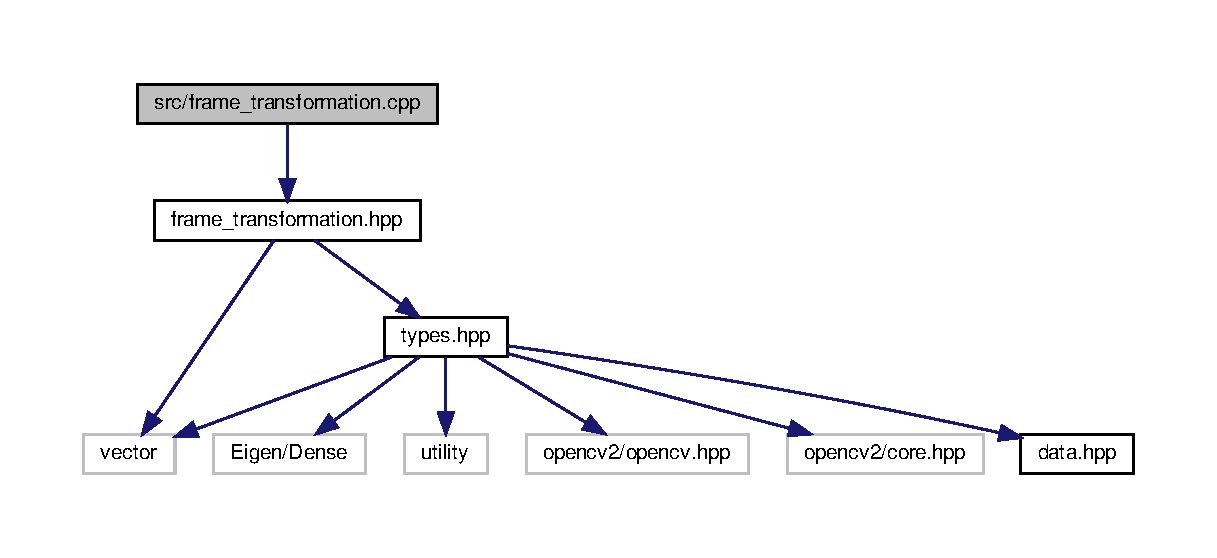
\includegraphics[width=350pt]{frame__transformation_8cpp__incl}
\end{center}
\end{figure}


\subsection{Detailed Description}
Performs frame transformation. 

M\+IT License

Copyright (c) 2021 Anubhav Paras, Sakshi Kakde, Siddharth Telang

Permission is hereby granted, free of charge, to any person obtaining a copy of this software and associated documentation files (the \char`\"{}\+Software\char`\"{}), to deal in the Software without restriction, including without limitation the rights to use, copy, modify, merge, publish, distribute, sublicense, and/or sell copies of the Software, and to permit persons to whom the Software is furnished to do so, subject to the following conditions\+:

The above copyright notice and this permission notice shall be included in all copies or substantial portions of the Software.

T\+HE S\+O\+F\+T\+W\+A\+RE IS P\+R\+O\+V\+I\+D\+ED \char`\"{}\+A\+S I\+S\char`\"{}, W\+I\+T\+H\+O\+UT W\+A\+R\+R\+A\+N\+TY OF A\+NY K\+I\+ND, E\+X\+P\+R\+E\+SS OR I\+M\+P\+L\+I\+ED, I\+N\+C\+L\+U\+D\+I\+NG B\+UT N\+OT L\+I\+M\+I\+T\+ED TO T\+HE W\+A\+R\+R\+A\+N\+T\+I\+ES OF M\+E\+R\+C\+H\+A\+N\+T\+A\+B\+I\+L\+I\+TY, F\+I\+T\+N\+E\+SS F\+OR A P\+A\+R\+T\+I\+C\+U\+L\+AR P\+U\+R\+P\+O\+SE A\+ND N\+O\+N\+I\+N\+F\+R\+I\+N\+G\+E\+M\+E\+NT. IN NO E\+V\+E\+NT S\+H\+A\+LL T\+HE A\+U\+T\+H\+O\+RS OR C\+O\+P\+Y\+R\+I\+G\+HT H\+O\+L\+D\+E\+RS BE L\+I\+A\+B\+LE F\+OR A\+NY C\+L\+A\+IM, D\+A\+M\+A\+G\+ES OR O\+T\+H\+ER L\+I\+A\+B\+I\+L\+I\+TY, W\+H\+E\+T\+H\+ER IN AN A\+C\+T\+I\+ON OF C\+O\+N\+T\+R\+A\+CT, T\+O\+RT OR O\+T\+H\+E\+R\+W\+I\+SE, A\+R\+I\+S\+I\+NG F\+R\+OM, O\+UT OF OR IN C\+O\+N\+N\+E\+C\+T\+I\+ON W\+I\+TH T\+HE S\+O\+F\+T\+W\+A\+RE OR T\+HE U\+SE OR O\+T\+H\+ER D\+E\+A\+L\+I\+N\+GS IN T\+HE S\+O\+F\+T\+W\+A\+RE.

\begin{DoxyAuthor}{Author}
Anubhav Paras (\href{mailto:anubhav@umd.edu}{\tt anubhav@umd.\+edu}) 

Sakshi Kakde (\href{mailto:sakshi@umd.edu}{\tt sakshi@umd.\+edu}) 

Siddharth Telang (\href{mailto:stelang@umd.edu}{\tt stelang@umd.\+edu}) 
\end{DoxyAuthor}
\begin{DoxyVersion}{Version}
0.\+1 
\end{DoxyVersion}
\begin{DoxyDate}{Date}
2021-\/10-\/25
\end{DoxyDate}
\begin{DoxyCopyright}{Copyright}
Copyright (c) 2021 
\end{DoxyCopyright}

\hypertarget{model_8cpp}{}\section{src/model.cpp File Reference}
\label{model_8cpp}\index{src/model.\+cpp@{src/model.\+cpp}}


Constructs \hyperlink{classSVMHumanClassifier}{S\+V\+M\+Human\+Classifier} model object.  


{\ttfamily \#include $<$model.\+hpp$>$}\newline
Include dependency graph for model.\+cpp\+:
\nopagebreak
\begin{figure}[H]
\begin{center}
\leavevmode
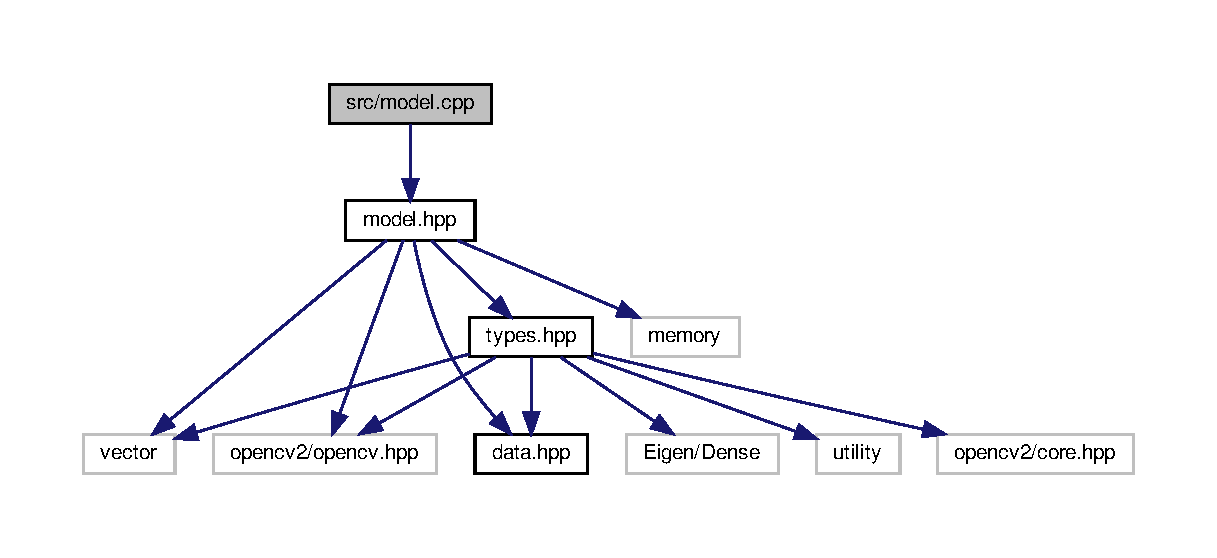
\includegraphics[width=350pt]{model_8cpp__incl}
\end{center}
\end{figure}


\subsection{Detailed Description}
Constructs \hyperlink{classSVMHumanClassifier}{S\+V\+M\+Human\+Classifier} model object. 

M\+IT License

Copyright (c) 2021 Anubhav Paras, Sakshi Kakde, Siddharth Telang

Permission is hereby granted, free of charge, to any person obtaining a copy of this software and associated documentation files (the \char`\"{}\+Software\char`\"{}), to deal in the Software without restriction, including without limitation the rights to use, copy, modify, merge, publish, distribute, sublicense, and/or sell copies of the Software, and to permit persons to whom the Software is furnished to do so, subject to the following conditions\+:

The above copyright notice and this permission notice shall be included in all copies or substantial portions of the Software.

T\+HE S\+O\+F\+T\+W\+A\+RE IS P\+R\+O\+V\+I\+D\+ED \char`\"{}\+A\+S I\+S\char`\"{}, W\+I\+T\+H\+O\+UT W\+A\+R\+R\+A\+N\+TY OF A\+NY K\+I\+ND, E\+X\+P\+R\+E\+SS OR I\+M\+P\+L\+I\+ED, I\+N\+C\+L\+U\+D\+I\+NG B\+UT N\+OT L\+I\+M\+I\+T\+ED TO T\+HE W\+A\+R\+R\+A\+N\+T\+I\+ES OF M\+E\+R\+C\+H\+A\+N\+T\+A\+B\+I\+L\+I\+TY, F\+I\+T\+N\+E\+SS F\+OR A P\+A\+R\+T\+I\+C\+U\+L\+AR P\+U\+R\+P\+O\+SE A\+ND N\+O\+N\+I\+N\+F\+R\+I\+N\+G\+E\+M\+E\+NT. IN NO E\+V\+E\+NT S\+H\+A\+LL T\+HE A\+U\+T\+H\+O\+RS OR C\+O\+P\+Y\+R\+I\+G\+HT H\+O\+L\+D\+E\+RS BE L\+I\+A\+B\+LE F\+OR A\+NY C\+L\+A\+IM, D\+A\+M\+A\+G\+ES OR O\+T\+H\+ER L\+I\+A\+B\+I\+L\+I\+TY, W\+H\+E\+T\+H\+ER IN AN A\+C\+T\+I\+ON OF C\+O\+N\+T\+R\+A\+CT, T\+O\+RT OR O\+T\+H\+E\+R\+W\+I\+SE, A\+R\+I\+S\+I\+NG F\+R\+OM, O\+UT OF OR IN C\+O\+N\+N\+E\+C\+T\+I\+ON W\+I\+TH T\+HE S\+O\+F\+T\+W\+A\+RE OR T\+HE U\+SE OR O\+T\+H\+ER D\+E\+A\+L\+I\+N\+GS IN T\+HE S\+O\+F\+T\+W\+A\+RE.

\begin{DoxyAuthor}{Author}
Anubhav Paras (\href{mailto:anubhav@umd.edu}{\tt anubhav@umd.\+edu}) 

Sakshi Kakde (\href{mailto:sakshi@umd.edu}{\tt sakshi@umd.\+edu}) 

Siddharth Telang (\href{mailto:stelang@umd.edu}{\tt stelang@umd.\+edu}) 
\end{DoxyAuthor}
\begin{DoxyVersion}{Version}
0.\+1 
\end{DoxyVersion}
\begin{DoxyDate}{Date}
2021-\/10-\/25
\end{DoxyDate}
\begin{DoxyCopyright}{Copyright}
Copyright (c) 2021 
\end{DoxyCopyright}

\hypertarget{preprocessor_8cpp}{}\section{src/preprocessor.cpp File Reference}
\label{preprocessor_8cpp}\index{src/preprocessor.\+cpp@{src/preprocessor.\+cpp}}


Preprocessor to resize the data.  


{\ttfamily \#include $<$preprocessor.\+hpp$>$}\newline
Include dependency graph for preprocessor.\+cpp\+:
\nopagebreak
\begin{figure}[H]
\begin{center}
\leavevmode
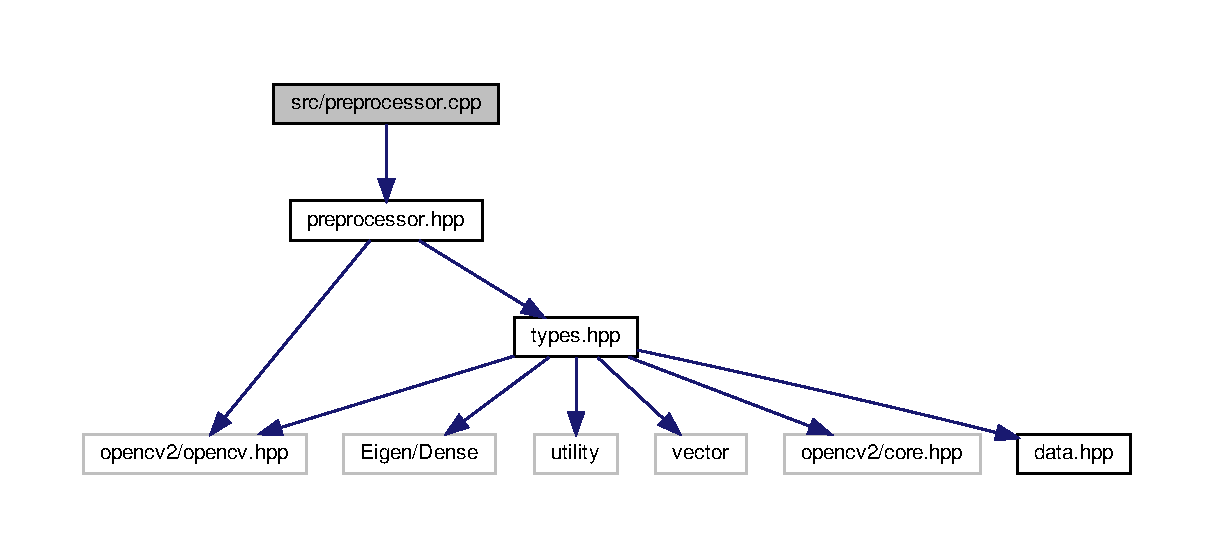
\includegraphics[width=350pt]{preprocessor_8cpp__incl}
\end{center}
\end{figure}


\subsection{Detailed Description}
Preprocessor to resize the data. 

M\+IT License

Copyright (c) 2021 Anubhav Paras, Sakshi Kakde, Siddharth Telang

Permission is hereby granted, free of charge, to any person obtaining a copy of this software and associated documentation files (the \char`\"{}\+Software\char`\"{}), to deal in the Software without restriction, including without limitation the rights to use, copy, modify, merge, publish, distribute, sublicense, and/or sell copies of the Software, and to permit persons to whom the Software is furnished to do so, subject to the following conditions\+:

The above copyright notice and this permission notice shall be included in all copies or substantial portions of the Software.

T\+HE S\+O\+F\+T\+W\+A\+RE IS P\+R\+O\+V\+I\+D\+ED \char`\"{}\+A\+S I\+S\char`\"{}, W\+I\+T\+H\+O\+UT W\+A\+R\+R\+A\+N\+TY OF A\+NY K\+I\+ND, E\+X\+P\+R\+E\+SS OR I\+M\+P\+L\+I\+ED, I\+N\+C\+L\+U\+D\+I\+NG B\+UT N\+OT L\+I\+M\+I\+T\+ED TO T\+HE W\+A\+R\+R\+A\+N\+T\+I\+ES OF M\+E\+R\+C\+H\+A\+N\+T\+A\+B\+I\+L\+I\+TY, F\+I\+T\+N\+E\+SS F\+OR A P\+A\+R\+T\+I\+C\+U\+L\+AR P\+U\+R\+P\+O\+SE A\+ND N\+O\+N\+I\+N\+F\+R\+I\+N\+G\+E\+M\+E\+NT. IN NO E\+V\+E\+NT S\+H\+A\+LL T\+HE A\+U\+T\+H\+O\+RS OR C\+O\+P\+Y\+R\+I\+G\+HT H\+O\+L\+D\+E\+RS BE L\+I\+A\+B\+LE F\+OR A\+NY C\+L\+A\+IM, D\+A\+M\+A\+G\+ES OR O\+T\+H\+ER L\+I\+A\+B\+I\+L\+I\+TY, W\+H\+E\+T\+H\+ER IN AN A\+C\+T\+I\+ON OF C\+O\+N\+T\+R\+A\+CT, T\+O\+RT OR O\+T\+H\+E\+R\+W\+I\+SE, A\+R\+I\+S\+I\+NG F\+R\+OM, O\+UT OF OR IN C\+O\+N\+N\+E\+C\+T\+I\+ON W\+I\+TH T\+HE S\+O\+F\+T\+W\+A\+RE OR T\+HE U\+SE OR O\+T\+H\+ER D\+E\+A\+L\+I\+N\+GS IN T\+HE S\+O\+F\+T\+W\+A\+RE.

\begin{DoxyAuthor}{Author}
Anubhav Paras (\href{mailto:anubhav@umd.edu}{\tt anubhav@umd.\+edu}) 

Sakshi Kakde (\href{mailto:sakshi@umd.edu}{\tt sakshi@umd.\+edu}) 

Siddharth Telang (\href{mailto:stelang@umd.edu}{\tt stelang@umd.\+edu}) 
\end{DoxyAuthor}
\begin{DoxyVersion}{Version}
0.\+1 
\end{DoxyVersion}
\begin{DoxyDate}{Date}
2021-\/10-\/25
\end{DoxyDate}
\begin{DoxyCopyright}{Copyright}
Copyright (c) 2021 
\end{DoxyCopyright}

\hypertarget{main_8cpp}{}\section{test/main.cpp File Reference}
\label{main_8cpp}\index{test/main.\+cpp@{test/main.\+cpp}}


runs all tests  


{\ttfamily \#include $<$gtest/gtest.\+h$>$}\newline
Include dependency graph for main.\+cpp\+:
\nopagebreak
\begin{figure}[H]
\begin{center}
\leavevmode
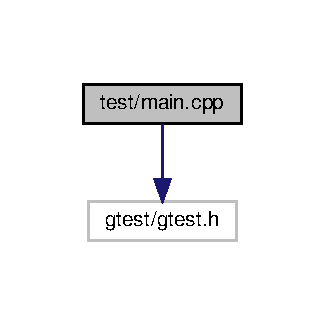
\includegraphics[width=156pt]{main_8cpp__incl}
\end{center}
\end{figure}
\subsection*{Functions}
\begin{DoxyCompactItemize}
\item 
\mbox{\Hypertarget{main_8cpp_a3c04138a5bfe5d72780bb7e82a18e627}\label{main_8cpp_a3c04138a5bfe5d72780bb7e82a18e627}} 
int {\bfseries main} (int argc, char $\ast$$\ast$argv)
\end{DoxyCompactItemize}


\subsection{Detailed Description}
runs all tests 

M\+IT License

Copyright (c) 2021 Anubhav Paras, Sakshi Kakde, Siddharth Telang

Permission is hereby granted, free of charge, to any person obtaining a copy of this software and associated documentation files (the \char`\"{}\+Software\char`\"{}), to deal in the Software without restriction, including without limitation the rights to use, copy, modify, merge, publish, distribute, sublicense, and/or sell copies of the Software, and to permit persons to whom the Software is furnished to do so, subject to the following conditions\+:

The above copyright notice and this permission notice shall be included in all copies or substantial portions of the Software.

T\+HE S\+O\+F\+T\+W\+A\+RE IS P\+R\+O\+V\+I\+D\+ED \char`\"{}\+A\+S I\+S\char`\"{}, W\+I\+T\+H\+O\+UT W\+A\+R\+R\+A\+N\+TY OF A\+NY K\+I\+ND, E\+X\+P\+R\+E\+SS OR I\+M\+P\+L\+I\+ED, I\+N\+C\+L\+U\+D\+I\+NG B\+UT N\+OT L\+I\+M\+I\+T\+ED TO T\+HE W\+A\+R\+R\+A\+N\+T\+I\+ES OF M\+E\+R\+C\+H\+A\+N\+T\+A\+B\+I\+L\+I\+TY, F\+I\+T\+N\+E\+SS F\+OR A P\+A\+R\+T\+I\+C\+U\+L\+AR P\+U\+R\+P\+O\+SE A\+ND N\+O\+N\+I\+N\+F\+R\+I\+N\+G\+E\+M\+E\+NT. IN NO E\+V\+E\+NT S\+H\+A\+LL T\+HE A\+U\+T\+H\+O\+RS OR C\+O\+P\+Y\+R\+I\+G\+HT H\+O\+L\+D\+E\+RS BE L\+I\+A\+B\+LE F\+OR A\+NY C\+L\+A\+IM, D\+A\+M\+A\+G\+ES OR O\+T\+H\+ER L\+I\+A\+B\+I\+L\+I\+TY, W\+H\+E\+T\+H\+ER IN AN A\+C\+T\+I\+ON OF C\+O\+N\+T\+R\+A\+CT, T\+O\+RT OR O\+T\+H\+E\+R\+W\+I\+SE, A\+R\+I\+S\+I\+NG F\+R\+OM, O\+UT OF OR IN C\+O\+N\+N\+E\+C\+T\+I\+ON W\+I\+TH T\+HE S\+O\+F\+T\+W\+A\+RE OR T\+HE U\+SE OR O\+T\+H\+ER D\+E\+A\+L\+I\+N\+GS IN T\+HE S\+O\+F\+T\+W\+A\+RE.

\begin{DoxyAuthor}{Author}
Anubhav Paras (\href{mailto:anubhav@umd.edu}{\tt anubhav@umd.\+edu}) 

Sakshi Kakde (\href{mailto:sakshi@umd.edu}{\tt sakshi@umd.\+edu}) 

Siddharth Telang (\href{mailto:stelang@umd.edu}{\tt stelang@umd.\+edu}) 
\end{DoxyAuthor}
\begin{DoxyVersion}{Version}
0.\+1 
\end{DoxyVersion}
\begin{DoxyDate}{Date}
2021-\/10-\/25
\end{DoxyDate}
\begin{DoxyCopyright}{Copyright}
Copyright (c) 2021 
\end{DoxyCopyright}

\hypertarget{test__data_8cpp}{}\section{test/test\+\_\+data.cpp File Reference}
\label{test__data_8cpp}\index{test/test\+\_\+data.\+cpp@{test/test\+\_\+data.\+cpp}}


test file for \hyperlink{data_8cpp}{data.\+cpp}  


{\ttfamily \#include $<$gtest/gtest.\+h$>$}\newline
{\ttfamily \#include $<$data.\+hpp$>$}\newline
Include dependency graph for test\+\_\+data.\+cpp\+:
\nopagebreak
\begin{figure}[H]
\begin{center}
\leavevmode
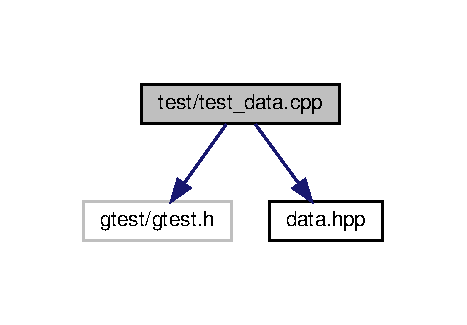
\includegraphics[width=224pt]{test__data_8cpp__incl}
\end{center}
\end{figure}
\subsection*{Functions}
\begin{DoxyCompactItemize}
\item 
\mbox{\Hypertarget{test__data_8cpp_a08e986bbe93f3e12651479ccddc09b9e}\label{test__data_8cpp_a08e986bbe93f3e12651479ccddc09b9e}} 
{\bfseries T\+E\+ST} (data\+\_\+test, test\+\_\+getter\+\_\+setter)
\item 
\mbox{\Hypertarget{test__data_8cpp_ab40f1c3e7046c8c72be65d37de33d506}\label{test__data_8cpp_ab40f1c3e7046c8c72be65d37de33d506}} 
{\bfseries T\+E\+ST} (data\+\_\+test, test\+\_\+param\+\_\+constructor)
\end{DoxyCompactItemize}


\subsection{Detailed Description}
test file for \hyperlink{data_8cpp}{data.\+cpp} 

M\+IT License

Copyright (c) 2021 Anubhav Paras, Sakshi Kakde, Siddharth Telang

Permission is hereby granted, free of charge, to any person obtaining a copy of this software and associated documentation files (the \char`\"{}\+Software\char`\"{}), to deal in the Software without restriction, including without limitation the rights to use, copy, modify, merge, publish, distribute, sublicense, and/or sell copies of the Software, and to permit persons to whom the Software is furnished to do so, subject to the following conditions\+:

The above copyright notice and this permission notice shall be included in all copies or substantial portions of the Software.

T\+HE S\+O\+F\+T\+W\+A\+RE IS P\+R\+O\+V\+I\+D\+ED \char`\"{}\+A\+S I\+S\char`\"{}, W\+I\+T\+H\+O\+UT W\+A\+R\+R\+A\+N\+TY OF A\+NY K\+I\+ND, E\+X\+P\+R\+E\+SS OR I\+M\+P\+L\+I\+ED, I\+N\+C\+L\+U\+D\+I\+NG B\+UT N\+OT L\+I\+M\+I\+T\+ED TO T\+HE W\+A\+R\+R\+A\+N\+T\+I\+ES OF M\+E\+R\+C\+H\+A\+N\+T\+A\+B\+I\+L\+I\+TY, F\+I\+T\+N\+E\+SS F\+OR A P\+A\+R\+T\+I\+C\+U\+L\+AR P\+U\+R\+P\+O\+SE A\+ND N\+O\+N\+I\+N\+F\+R\+I\+N\+G\+E\+M\+E\+NT. IN NO E\+V\+E\+NT S\+H\+A\+LL T\+HE A\+U\+T\+H\+O\+RS OR C\+O\+P\+Y\+R\+I\+G\+HT H\+O\+L\+D\+E\+RS BE L\+I\+A\+B\+LE F\+OR A\+NY C\+L\+A\+IM, D\+A\+M\+A\+G\+ES OR O\+T\+H\+ER L\+I\+A\+B\+I\+L\+I\+TY, W\+H\+E\+T\+H\+ER IN AN A\+C\+T\+I\+ON OF C\+O\+N\+T\+R\+A\+CT, T\+O\+RT OR O\+T\+H\+E\+R\+W\+I\+SE, A\+R\+I\+S\+I\+NG F\+R\+OM, O\+UT OF OR IN C\+O\+N\+N\+E\+C\+T\+I\+ON W\+I\+TH T\+HE S\+O\+F\+T\+W\+A\+RE OR T\+HE U\+SE OR O\+T\+H\+ER D\+E\+A\+L\+I\+N\+GS IN T\+HE S\+O\+F\+T\+W\+A\+RE.

\begin{DoxyAuthor}{Author}
Anubhav Paras (\href{mailto:anubhav@umd.edu}{\tt anubhav@umd.\+edu}) 

Sakshi Kakde (\href{mailto:sakshi@umd.edu}{\tt sakshi@umd.\+edu}) 

Siddharth Telang (\href{mailto:stelang@umd.edu}{\tt stelang@umd.\+edu}) 
\end{DoxyAuthor}
\begin{DoxyVersion}{Version}
0.\+1 
\end{DoxyVersion}
\begin{DoxyDate}{Date}
2021-\/10-\/25
\end{DoxyDate}
\begin{DoxyCopyright}{Copyright}
Copyright (c) 2021 
\end{DoxyCopyright}

\hypertarget{test__datareader_8cpp}{}\section{test/test\+\_\+datareader.cpp File Reference}
\label{test__datareader_8cpp}\index{test/test\+\_\+datareader.\+cpp@{test/test\+\_\+datareader.\+cpp}}


test file for \hyperlink{datareader_8cpp}{datareader.\+cpp}  


{\ttfamily \#include $<$gtest/gtest.\+h$>$}\newline
{\ttfamily \#include $<$string$>$}\newline
{\ttfamily \#include $<$datareader.\+hpp$>$}\newline
Include dependency graph for test\+\_\+datareader.\+cpp\+:
\nopagebreak
\begin{figure}[H]
\begin{center}
\leavevmode
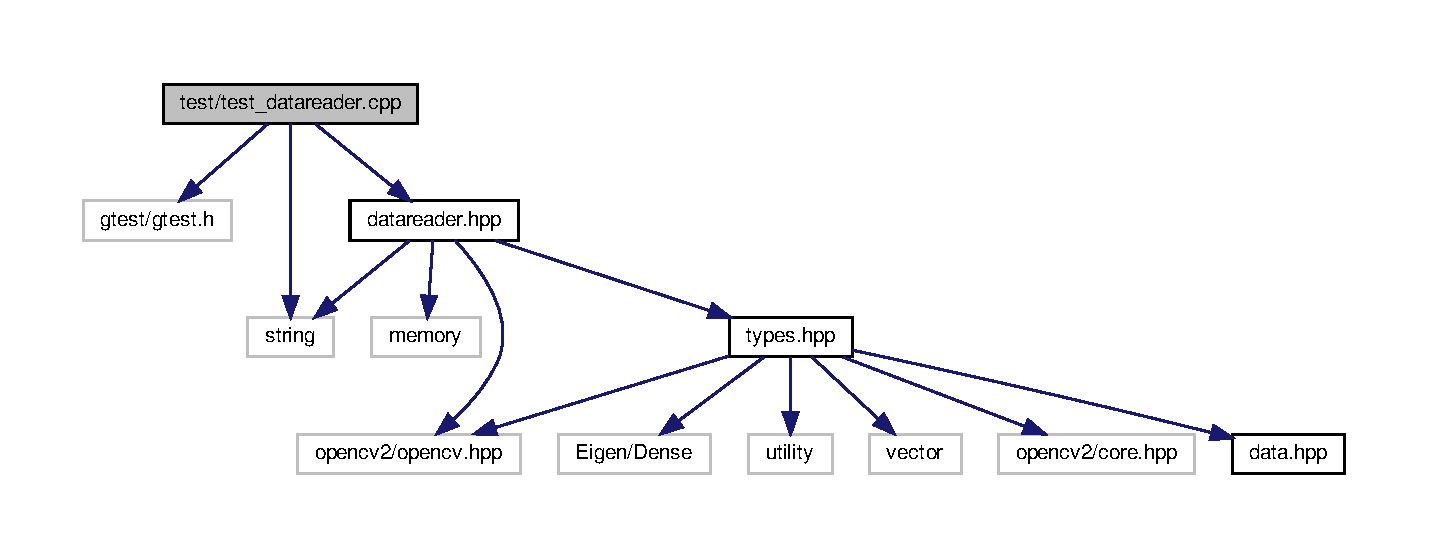
\includegraphics[width=350pt]{test__datareader_8cpp__incl}
\end{center}
\end{figure}
\subsection*{Functions}
\begin{DoxyCompactItemize}
\item 
\mbox{\Hypertarget{test__datareader_8cpp_a7454da40ceb0c8ee6352fb68076a226b}\label{test__datareader_8cpp_a7454da40ceb0c8ee6352fb68076a226b}} 
{\bfseries T\+E\+ST} (image\+\_\+reader\+\_\+test, image\+\_\+read\+\_\+success)
\end{DoxyCompactItemize}


\subsection{Detailed Description}
test file for \hyperlink{datareader_8cpp}{datareader.\+cpp} 

M\+IT License

Copyright (c) 2021 Anubhav Paras, Sakshi Kakde, Siddharth Telang

Permission is hereby granted, free of charge, to any person obtaining a copy of this software and associated documentation files (the \char`\"{}\+Software\char`\"{}), to deal in the Software without restriction, including without limitation the rights to use, copy, modify, merge, publish, distribute, sublicense, and/or sell copies of the Software, and to permit persons to whom the Software is furnished to do so, subject to the following conditions\+:

The above copyright notice and this permission notice shall be included in all copies or substantial portions of the Software.

T\+HE S\+O\+F\+T\+W\+A\+RE IS P\+R\+O\+V\+I\+D\+ED \char`\"{}\+A\+S I\+S\char`\"{}, W\+I\+T\+H\+O\+UT W\+A\+R\+R\+A\+N\+TY OF A\+NY K\+I\+ND, E\+X\+P\+R\+E\+SS OR I\+M\+P\+L\+I\+ED, I\+N\+C\+L\+U\+D\+I\+NG B\+UT N\+OT L\+I\+M\+I\+T\+ED TO T\+HE W\+A\+R\+R\+A\+N\+T\+I\+ES OF M\+E\+R\+C\+H\+A\+N\+T\+A\+B\+I\+L\+I\+TY, F\+I\+T\+N\+E\+SS F\+OR A P\+A\+R\+T\+I\+C\+U\+L\+AR P\+U\+R\+P\+O\+SE A\+ND N\+O\+N\+I\+N\+F\+R\+I\+N\+G\+E\+M\+E\+NT. IN NO E\+V\+E\+NT S\+H\+A\+LL T\+HE A\+U\+T\+H\+O\+RS OR C\+O\+P\+Y\+R\+I\+G\+HT H\+O\+L\+D\+E\+RS BE L\+I\+A\+B\+LE F\+OR A\+NY C\+L\+A\+IM, D\+A\+M\+A\+G\+ES OR O\+T\+H\+ER L\+I\+A\+B\+I\+L\+I\+TY, W\+H\+E\+T\+H\+ER IN AN A\+C\+T\+I\+ON OF C\+O\+N\+T\+R\+A\+CT, T\+O\+RT OR O\+T\+H\+E\+R\+W\+I\+SE, A\+R\+I\+S\+I\+NG F\+R\+OM, O\+UT OF OR IN C\+O\+N\+N\+E\+C\+T\+I\+ON W\+I\+TH T\+HE S\+O\+F\+T\+W\+A\+RE OR T\+HE U\+SE OR O\+T\+H\+ER D\+E\+A\+L\+I\+N\+GS IN T\+HE S\+O\+F\+T\+W\+A\+RE.

\begin{DoxyAuthor}{Author}
Anubhav Paras (\href{mailto:anubhav@umd.edu}{\tt anubhav@umd.\+edu}) 

Sakshi Kakde (\href{mailto:sakshi@umd.edu}{\tt sakshi@umd.\+edu}) 

Siddharth Telang (\href{mailto:stelang@umd.edu}{\tt stelang@umd.\+edu}) 
\end{DoxyAuthor}
\begin{DoxyVersion}{Version}
0.\+1 
\end{DoxyVersion}
\begin{DoxyDate}{Date}
2021-\/10-\/25
\end{DoxyDate}
\begin{DoxyCopyright}{Copyright}
Copyright (c) 2021 
\end{DoxyCopyright}

\hypertarget{test__detector_8cpp}{}\section{test/test\+\_\+detector.cpp File Reference}
\label{test__detector_8cpp}\index{test/test\+\_\+detector.\+cpp@{test/test\+\_\+detector.\+cpp}}


test file for \hyperlink{detector_8cpp}{detector.\+cpp}  


{\ttfamily \#include $<$gtest/gtest.\+h$>$}\newline
{\ttfamily \#include $<$gmock/gmock.\+h$>$}\newline
{\ttfamily \#include $<$memory$>$}\newline
{\ttfamily \#include $<$detector.\+hpp$>$}\newline
{\ttfamily \#include $<$mock/mock\+\_\+model.\+hpp$>$}\newline
{\ttfamily \#include $<$mock/mock\+\_\+frame\+\_\+transformation.\+hpp$>$}\newline
Include dependency graph for test\+\_\+detector.\+cpp\+:
\nopagebreak
\begin{figure}[H]
\begin{center}
\leavevmode
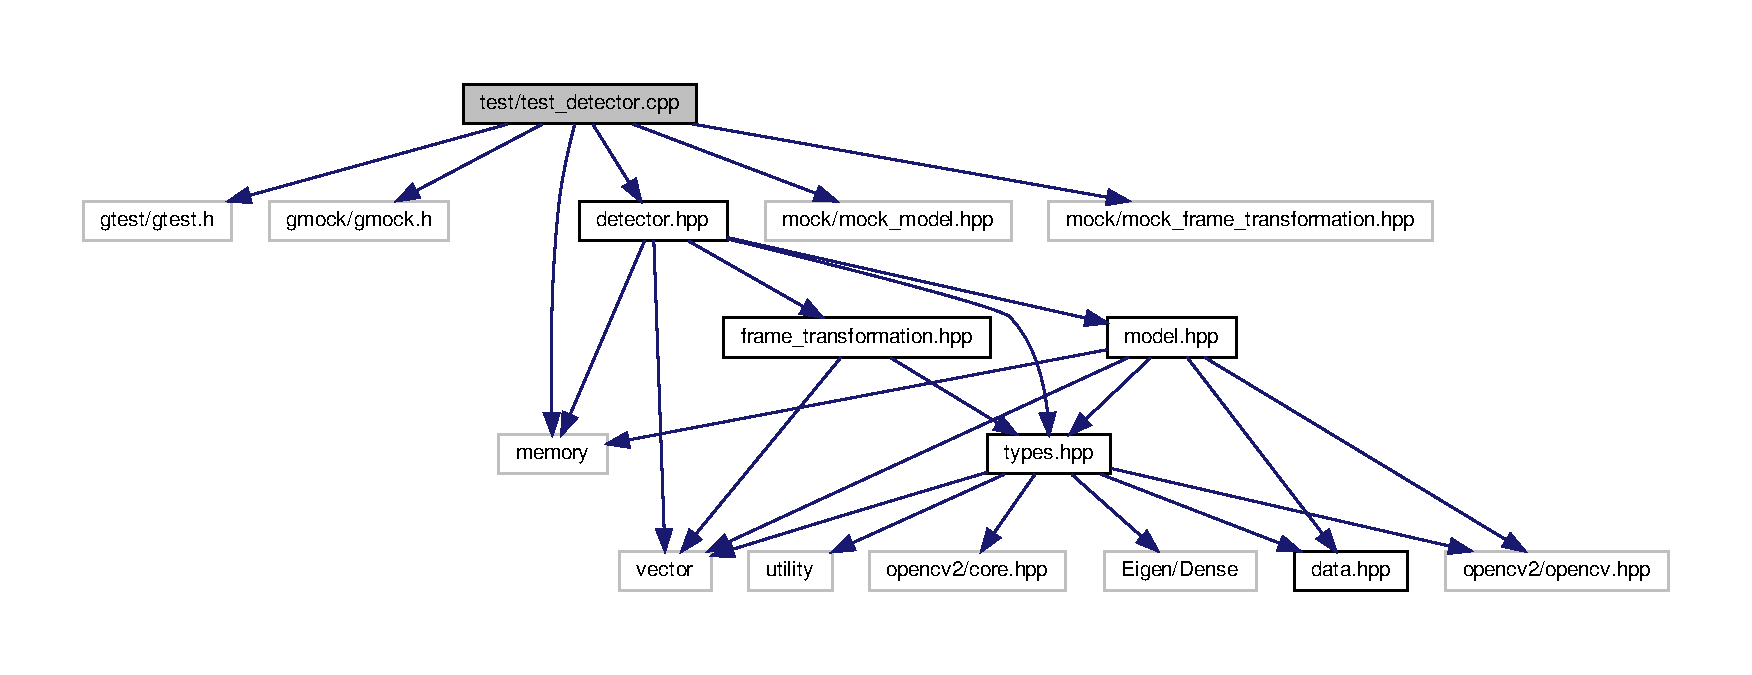
\includegraphics[width=350pt]{test__detector_8cpp__incl}
\end{center}
\end{figure}
\subsection*{Functions}
\begin{DoxyCompactItemize}
\item 
\mbox{\Hypertarget{test__detector_8cpp_a9f40ee8adbbb004881b44ad9efd0a9a6}\label{test__detector_8cpp_a9f40ee8adbbb004881b44ad9efd0a9a6}} 
{\bfseries T\+E\+ST} (detector\+\_\+test, test\+\_\+detect)
\item 
\mbox{\Hypertarget{test__detector_8cpp_ad63d5a2a919f420fcc68eea7506ef842}\label{test__detector_8cpp_ad63d5a2a919f420fcc68eea7506ef842}} 
{\bfseries T\+E\+ST} (detector\+\_\+test, test\+\_\+detect\+\_\+no\+\_\+boundingbox)
\item 
\mbox{\Hypertarget{test__detector_8cpp_af518c255790d30d595dec4adcb2509fc}\label{test__detector_8cpp_af518c255790d30d595dec4adcb2509fc}} 
{\bfseries T\+E\+ST} (detector\+\_\+test, test\+\_\+evaluate\+\_\+no\+\_\+boundingbox)
\item 
\mbox{\Hypertarget{test__detector_8cpp_a7e3a646331b76d17112de32fec50eb73}\label{test__detector_8cpp_a7e3a646331b76d17112de32fec50eb73}} 
{\bfseries T\+E\+ST} (detector\+\_\+test, test\+\_\+evaluate\+\_\+no\+\_\+gt\+\_\+centroids)
\item 
\mbox{\Hypertarget{test__detector_8cpp_ad2794a1ee15d37f075247ab9791ffc46}\label{test__detector_8cpp_ad2794a1ee15d37f075247ab9791ffc46}} 
{\bfseries T\+E\+ST} (detector\+\_\+test, test\+\_\+evaluate\+\_\+model)
\end{DoxyCompactItemize}


\subsection{Detailed Description}
test file for \hyperlink{detector_8cpp}{detector.\+cpp} 

M\+IT License

Copyright (c) 2021 Anubhav Paras, Sakshi Kakde, Siddharth Telang

Permission is hereby granted, free of charge, to any person obtaining a copy of this software and associated documentation files (the \char`\"{}\+Software\char`\"{}), to deal in the Software without restriction, including without limitation the rights to use, copy, modify, merge, publish, distribute, sublicense, and/or sell copies of the Software, and to permit persons to whom the Software is furnished to do so, subject to the following conditions\+:

The above copyright notice and this permission notice shall be included in all copies or substantial portions of the Software.

T\+HE S\+O\+F\+T\+W\+A\+RE IS P\+R\+O\+V\+I\+D\+ED \char`\"{}\+A\+S I\+S\char`\"{}, W\+I\+T\+H\+O\+UT W\+A\+R\+R\+A\+N\+TY OF A\+NY K\+I\+ND, E\+X\+P\+R\+E\+SS OR I\+M\+P\+L\+I\+ED, I\+N\+C\+L\+U\+D\+I\+NG B\+UT N\+OT L\+I\+M\+I\+T\+ED TO T\+HE W\+A\+R\+R\+A\+N\+T\+I\+ES OF M\+E\+R\+C\+H\+A\+N\+T\+A\+B\+I\+L\+I\+TY, F\+I\+T\+N\+E\+SS F\+OR A P\+A\+R\+T\+I\+C\+U\+L\+AR P\+U\+R\+P\+O\+SE A\+ND N\+O\+N\+I\+N\+F\+R\+I\+N\+G\+E\+M\+E\+NT. IN NO E\+V\+E\+NT S\+H\+A\+LL T\+HE A\+U\+T\+H\+O\+RS OR C\+O\+P\+Y\+R\+I\+G\+HT H\+O\+L\+D\+E\+RS BE L\+I\+A\+B\+LE F\+OR A\+NY C\+L\+A\+IM, D\+A\+M\+A\+G\+ES OR O\+T\+H\+ER L\+I\+A\+B\+I\+L\+I\+TY, W\+H\+E\+T\+H\+ER IN AN A\+C\+T\+I\+ON OF C\+O\+N\+T\+R\+A\+CT, T\+O\+RT OR O\+T\+H\+E\+R\+W\+I\+SE, A\+R\+I\+S\+I\+NG F\+R\+OM, O\+UT OF OR IN C\+O\+N\+N\+E\+C\+T\+I\+ON W\+I\+TH T\+HE S\+O\+F\+T\+W\+A\+RE OR T\+HE U\+SE OR O\+T\+H\+ER D\+E\+A\+L\+I\+N\+GS IN T\+HE S\+O\+F\+T\+W\+A\+RE.

\begin{DoxyAuthor}{Author}
Anubhav Paras (\href{mailto:anubhav@umd.edu}{\tt anubhav@umd.\+edu}) 

Sakshi Kakde (\href{mailto:sakshi@umd.edu}{\tt sakshi@umd.\+edu}) 

Siddharth Telang (\href{mailto:stelang@umd.edu}{\tt stelang@umd.\+edu}) 
\end{DoxyAuthor}
\begin{DoxyVersion}{Version}
0.\+1 
\end{DoxyVersion}
\begin{DoxyDate}{Date}
2021-\/10-\/25
\end{DoxyDate}
\begin{DoxyCopyright}{Copyright}
Copyright (c) 2021 
\end{DoxyCopyright}

\hypertarget{test__driver_8cpp}{}\section{test/test\+\_\+driver.cpp File Reference}
\label{test__driver_8cpp}\index{test/test\+\_\+driver.\+cpp@{test/test\+\_\+driver.\+cpp}}


test file for \hyperlink{driver_8cpp}{driver.\+cpp}  


{\ttfamily \#include $<$gtest/gtest.\+h$>$}\newline
{\ttfamily \#include $<$gmock/gmock.\+h$>$}\newline
{\ttfamily \#include $<$memory$>$}\newline
{\ttfamily \#include $<$driver.\+hpp$>$}\newline
{\ttfamily \#include $<$mock/mock\+\_\+datareader.\+hpp$>$}\newline
{\ttfamily \#include $<$mock/mock\+\_\+preprocessor.\+hpp$>$}\newline
{\ttfamily \#include $<$mock/mock\+\_\+detector.\+hpp$>$}\newline
Include dependency graph for test\+\_\+driver.\+cpp\+:
\nopagebreak
\begin{figure}[H]
\begin{center}
\leavevmode
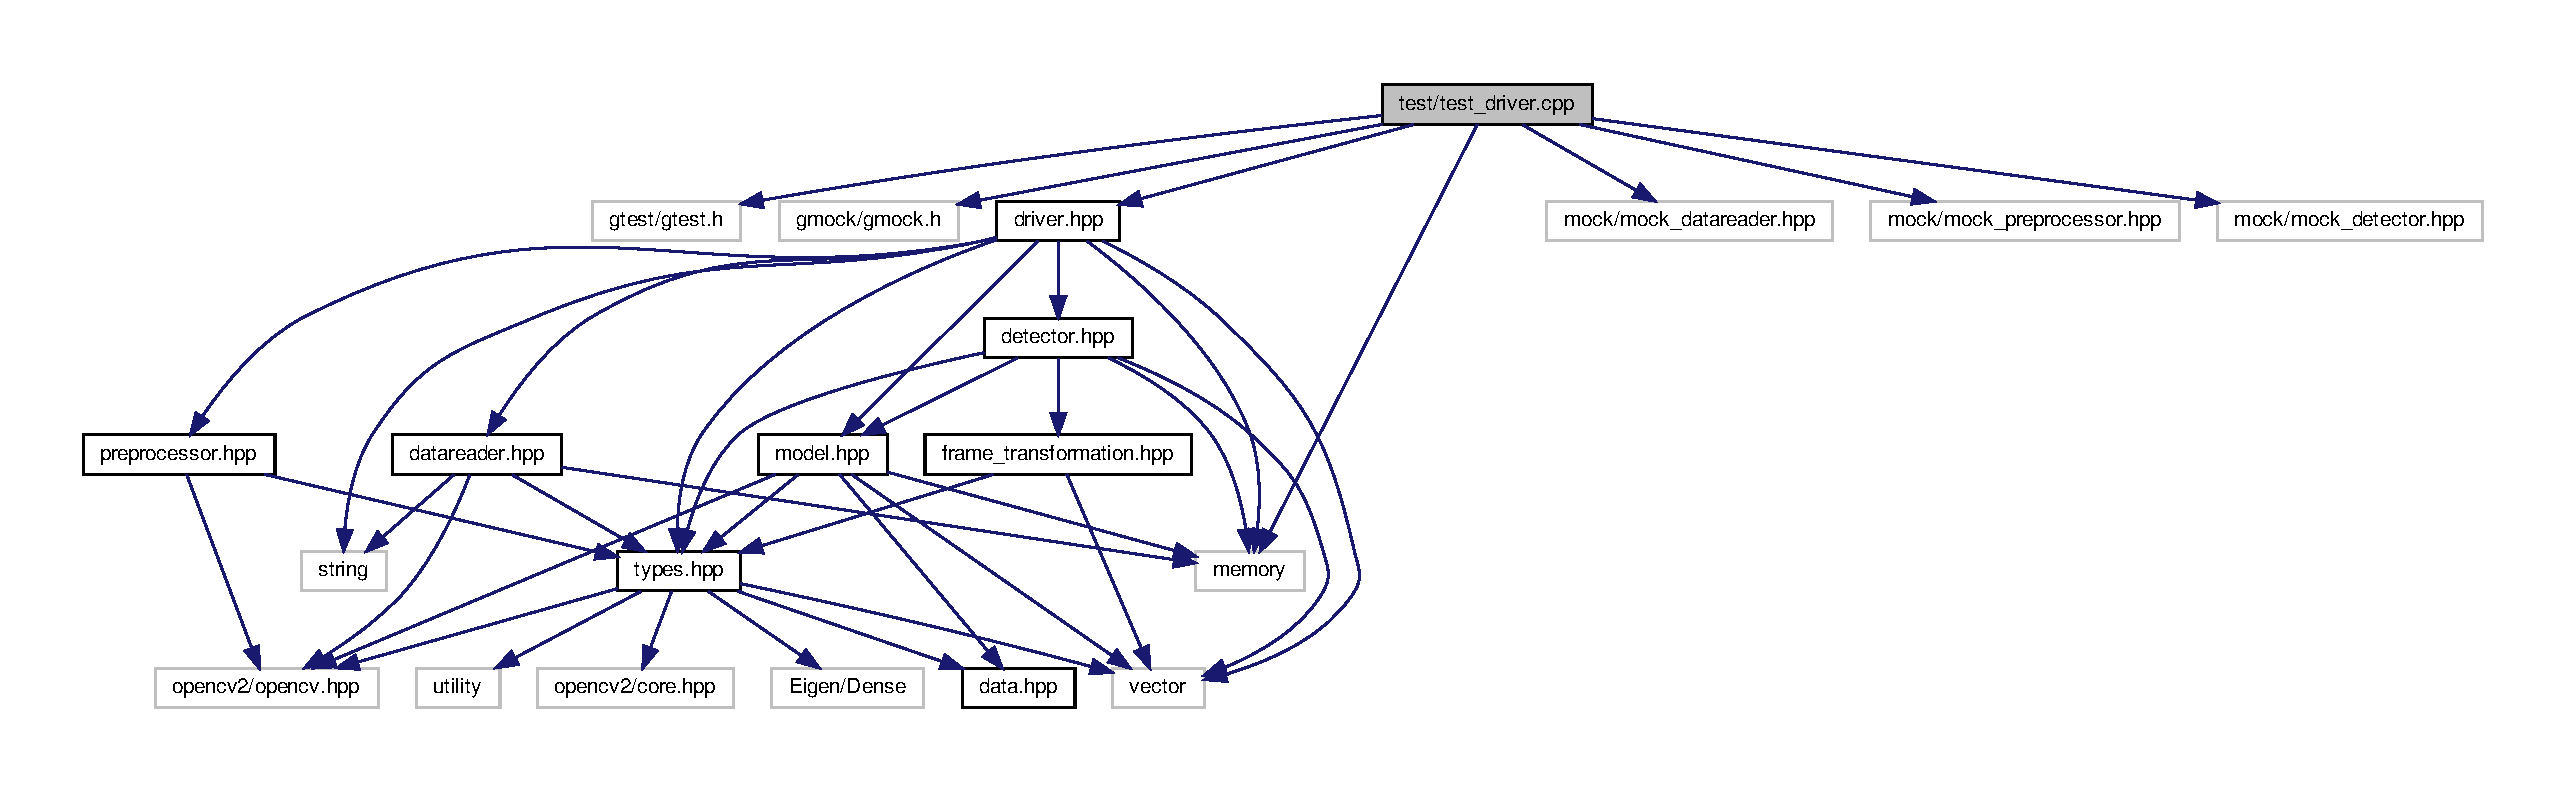
\includegraphics[width=350pt]{test__driver_8cpp__incl}
\end{center}
\end{figure}
\subsection*{Functions}
\begin{DoxyCompactItemize}
\item 
\mbox{\Hypertarget{test__driver_8cpp_a2f3e989dfc3216c75cf5fc3458c2e37f}\label{test__driver_8cpp_a2f3e989dfc3216c75cf5fc3458c2e37f}} 
{\bfseries T\+E\+ST} (driver\+\_\+test, test\+\_\+execute\+Detection\+Pipe\+Line)
\item 
\mbox{\Hypertarget{test__driver_8cpp_a622a086f9eb15bcca7bdd89c5c866da5}\label{test__driver_8cpp_a622a086f9eb15bcca7bdd89c5c866da5}} 
{\bfseries T\+E\+ST} (driver\+\_\+test, test\+\_\+evaluate\+\_\+model)
\end{DoxyCompactItemize}


\subsection{Detailed Description}
test file for \hyperlink{driver_8cpp}{driver.\+cpp} 

M\+IT License

Copyright (c) 2021 Anubhav Paras, Sakshi Kakde, Siddharth Telang

Permission is hereby granted, free of charge, to any person obtaining a copy of this software and associated documentation files (the \char`\"{}\+Software\char`\"{}), to deal in the Software without restriction, including without limitation the rights to use, copy, modify, merge, publish, distribute, sublicense, and/or sell copies of the Software, and to permit persons to whom the Software is furnished to do so, subject to the following conditions\+:

The above copyright notice and this permission notice shall be included in all copies or substantial portions of the Software.

T\+HE S\+O\+F\+T\+W\+A\+RE IS P\+R\+O\+V\+I\+D\+ED \char`\"{}\+A\+S I\+S\char`\"{}, W\+I\+T\+H\+O\+UT W\+A\+R\+R\+A\+N\+TY OF A\+NY K\+I\+ND, E\+X\+P\+R\+E\+SS OR I\+M\+P\+L\+I\+ED, I\+N\+C\+L\+U\+D\+I\+NG B\+UT N\+OT L\+I\+M\+I\+T\+ED TO T\+HE W\+A\+R\+R\+A\+N\+T\+I\+ES OF M\+E\+R\+C\+H\+A\+N\+T\+A\+B\+I\+L\+I\+TY, F\+I\+T\+N\+E\+SS F\+OR A P\+A\+R\+T\+I\+C\+U\+L\+AR P\+U\+R\+P\+O\+SE A\+ND N\+O\+N\+I\+N\+F\+R\+I\+N\+G\+E\+M\+E\+NT. IN NO E\+V\+E\+NT S\+H\+A\+LL T\+HE A\+U\+T\+H\+O\+RS OR C\+O\+P\+Y\+R\+I\+G\+HT H\+O\+L\+D\+E\+RS BE L\+I\+A\+B\+LE F\+OR A\+NY C\+L\+A\+IM, D\+A\+M\+A\+G\+ES OR O\+T\+H\+ER L\+I\+A\+B\+I\+L\+I\+TY, W\+H\+E\+T\+H\+ER IN AN A\+C\+T\+I\+ON OF C\+O\+N\+T\+R\+A\+CT, T\+O\+RT OR O\+T\+H\+E\+R\+W\+I\+SE, A\+R\+I\+S\+I\+NG F\+R\+OM, O\+UT OF OR IN C\+O\+N\+N\+E\+C\+T\+I\+ON W\+I\+TH T\+HE S\+O\+F\+T\+W\+A\+RE OR T\+HE U\+SE OR O\+T\+H\+ER D\+E\+A\+L\+I\+N\+GS IN T\+HE S\+O\+F\+T\+W\+A\+RE.

\begin{DoxyAuthor}{Author}
Anubhav Paras (\href{mailto:anubhav@umd.edu}{\tt anubhav@umd.\+edu}) 

Sakshi Kakde (\href{mailto:sakshi@umd.edu}{\tt sakshi@umd.\+edu}) 

Siddharth Telang (\href{mailto:stelang@umd.edu}{\tt stelang@umd.\+edu}) 
\end{DoxyAuthor}
\begin{DoxyVersion}{Version}
0.\+1 
\end{DoxyVersion}
\begin{DoxyDate}{Date}
2021-\/10-\/25
\end{DoxyDate}
\begin{DoxyCopyright}{Copyright}
Copyright (c) 2021 
\end{DoxyCopyright}

\hypertarget{test__frame__transformation_8cpp}{}\section{test/test\+\_\+frame\+\_\+transformation.cpp File Reference}
\label{test__frame__transformation_8cpp}\index{test/test\+\_\+frame\+\_\+transformation.\+cpp@{test/test\+\_\+frame\+\_\+transformation.\+cpp}}


test file for \hyperlink{frame__transformation_8cpp}{frame\+\_\+transformation.\+cpp}  


{\ttfamily \#include $<$gtest/gtest.\+h$>$}\newline
{\ttfamily \#include $<$string$>$}\newline
{\ttfamily \#include $<$frame\+\_\+transformation.\+hpp$>$}\newline
Include dependency graph for test\+\_\+frame\+\_\+transformation.\+cpp\+:
\nopagebreak
\begin{figure}[H]
\begin{center}
\leavevmode
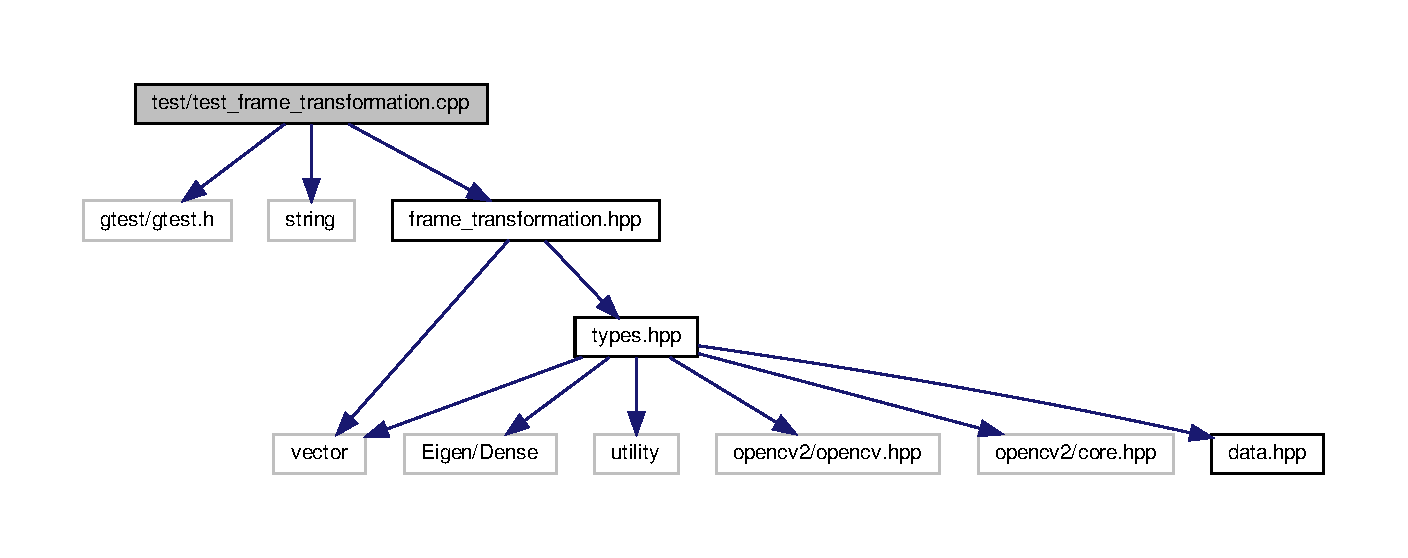
\includegraphics[width=350pt]{test__frame__transformation_8cpp__incl}
\end{center}
\end{figure}
\subsection*{Functions}
\begin{DoxyCompactItemize}
\item 
\mbox{\Hypertarget{test__frame__transformation_8cpp_a8949555886471f11f3f3682f42a53f0e}\label{test__frame__transformation_8cpp_a8949555886471f11f3f3682f42a53f0e}} 
{\bfseries T\+E\+ST} (frame\+\_\+transformation\+\_\+test, check\+\_\+frame\+\_\+transformation)
\end{DoxyCompactItemize}


\subsection{Detailed Description}
test file for \hyperlink{frame__transformation_8cpp}{frame\+\_\+transformation.\+cpp} 

M\+IT License

Copyright (c) 2021 Anubhav Paras, Sakshi Kakde, Siddharth Telang

Permission is hereby granted, free of charge, to any person obtaining a copy of this software and associated documentation files (the \char`\"{}\+Software\char`\"{}), to deal in the Software without restriction, including without limitation the rights to use, copy, modify, merge, publish, distribute, sublicense, and/or sell copies of the Software, and to permit persons to whom the Software is furnished to do so, subject to the following conditions\+:

The above copyright notice and this permission notice shall be included in all copies or substantial portions of the Software.

T\+HE S\+O\+F\+T\+W\+A\+RE IS P\+R\+O\+V\+I\+D\+ED \char`\"{}\+A\+S I\+S\char`\"{}, W\+I\+T\+H\+O\+UT W\+A\+R\+R\+A\+N\+TY OF A\+NY K\+I\+ND, E\+X\+P\+R\+E\+SS OR I\+M\+P\+L\+I\+ED, I\+N\+C\+L\+U\+D\+I\+NG B\+UT N\+OT L\+I\+M\+I\+T\+ED TO T\+HE W\+A\+R\+R\+A\+N\+T\+I\+ES OF M\+E\+R\+C\+H\+A\+N\+T\+A\+B\+I\+L\+I\+TY, F\+I\+T\+N\+E\+SS F\+OR A P\+A\+R\+T\+I\+C\+U\+L\+AR P\+U\+R\+P\+O\+SE A\+ND N\+O\+N\+I\+N\+F\+R\+I\+N\+G\+E\+M\+E\+NT. IN NO E\+V\+E\+NT S\+H\+A\+LL T\+HE A\+U\+T\+H\+O\+RS OR C\+O\+P\+Y\+R\+I\+G\+HT H\+O\+L\+D\+E\+RS BE L\+I\+A\+B\+LE F\+OR A\+NY C\+L\+A\+IM, D\+A\+M\+A\+G\+ES OR O\+T\+H\+ER L\+I\+A\+B\+I\+L\+I\+TY, W\+H\+E\+T\+H\+ER IN AN A\+C\+T\+I\+ON OF C\+O\+N\+T\+R\+A\+CT, T\+O\+RT OR O\+T\+H\+E\+R\+W\+I\+SE, A\+R\+I\+S\+I\+NG F\+R\+OM, O\+UT OF OR IN C\+O\+N\+N\+E\+C\+T\+I\+ON W\+I\+TH T\+HE S\+O\+F\+T\+W\+A\+RE OR T\+HE U\+SE OR O\+T\+H\+ER D\+E\+A\+L\+I\+N\+GS IN T\+HE S\+O\+F\+T\+W\+A\+RE.

\begin{DoxyAuthor}{Author}
Anubhav Paras (\href{mailto:anubhav@umd.edu}{\tt anubhav@umd.\+edu}) 

Sakshi Kakde (\href{mailto:sakshi@umd.edu}{\tt sakshi@umd.\+edu}) 

Siddharth Telang (\href{mailto:stelang@umd.edu}{\tt stelang@umd.\+edu}) 
\end{DoxyAuthor}
\begin{DoxyVersion}{Version}
0.\+1 
\end{DoxyVersion}
\begin{DoxyDate}{Date}
2021-\/10-\/25
\end{DoxyDate}
\begin{DoxyCopyright}{Copyright}
Copyright (c) 2021 
\end{DoxyCopyright}

\hypertarget{test__model_8cpp}{}\section{test/test\+\_\+model.cpp File Reference}
\label{test__model_8cpp}\index{test/test\+\_\+model.\+cpp@{test/test\+\_\+model.\+cpp}}


test file for \hyperlink{model_8cpp}{model.\+cpp}  


{\ttfamily \#include $<$gtest/gtest.\+h$>$}\newline
{\ttfamily \#include $<$string$>$}\newline
{\ttfamily \#include $<$opencv2/opencv.\+hpp$>$}\newline
{\ttfamily \#include $<$model.\+hpp$>$}\newline
Include dependency graph for test\+\_\+model.\+cpp\+:
\nopagebreak
\begin{figure}[H]
\begin{center}
\leavevmode
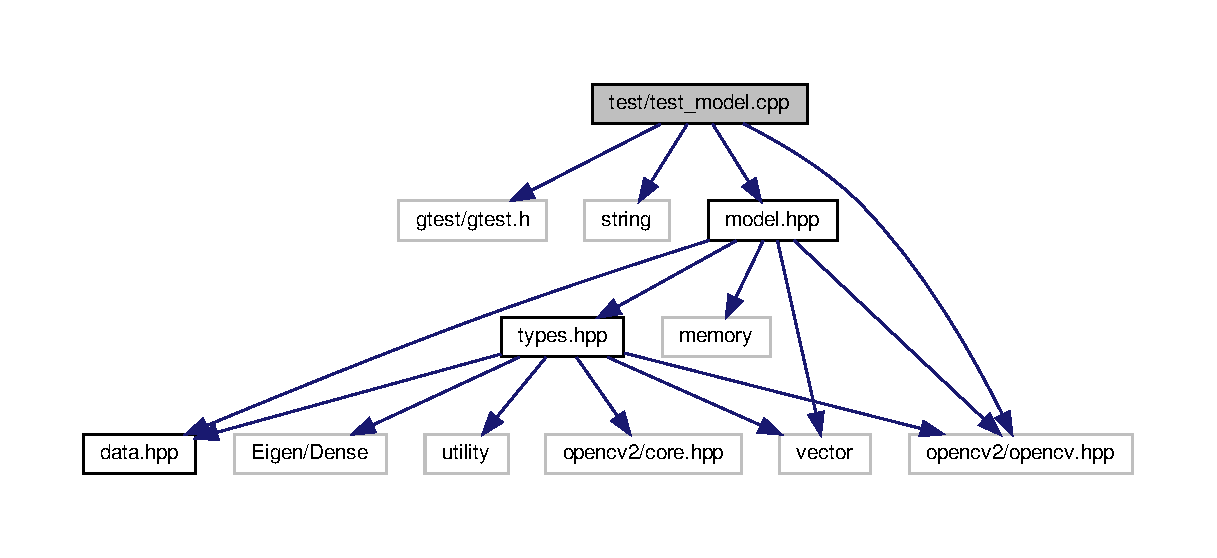
\includegraphics[width=350pt]{test__model_8cpp__incl}
\end{center}
\end{figure}
\subsection*{Functions}
\begin{DoxyCompactItemize}
\item 
\mbox{\Hypertarget{test__model_8cpp_ab992fb8d86fbbe26e42543d25721443c}\label{test__model_8cpp_ab992fb8d86fbbe26e42543d25721443c}} 
{\bfseries T\+E\+ST} (svm\+\_\+model\+\_\+test, check\+\_\+prediction\+\_\+with\+\_\+human)
\end{DoxyCompactItemize}


\subsection{Detailed Description}
test file for \hyperlink{model_8cpp}{model.\+cpp} 

M\+IT License

Copyright (c) 2021 Anubhav Paras, Sakshi Kakde, Siddharth Telang

Permission is hereby granted, free of charge, to any person obtaining a copy of this software and associated documentation files (the \char`\"{}\+Software\char`\"{}), to deal in the Software without restriction, including without limitation the rights to use, copy, modify, merge, publish, distribute, sublicense, and/or sell copies of the Software, and to permit persons to whom the Software is furnished to do so, subject to the following conditions\+:

The above copyright notice and this permission notice shall be included in all copies or substantial portions of the Software.

T\+HE S\+O\+F\+T\+W\+A\+RE IS P\+R\+O\+V\+I\+D\+ED \char`\"{}\+A\+S I\+S\char`\"{}, W\+I\+T\+H\+O\+UT W\+A\+R\+R\+A\+N\+TY OF A\+NY K\+I\+ND, E\+X\+P\+R\+E\+SS OR I\+M\+P\+L\+I\+ED, I\+N\+C\+L\+U\+D\+I\+NG B\+UT N\+OT L\+I\+M\+I\+T\+ED TO T\+HE W\+A\+R\+R\+A\+N\+T\+I\+ES OF M\+E\+R\+C\+H\+A\+N\+T\+A\+B\+I\+L\+I\+TY, F\+I\+T\+N\+E\+SS F\+OR A P\+A\+R\+T\+I\+C\+U\+L\+AR P\+U\+R\+P\+O\+SE A\+ND N\+O\+N\+I\+N\+F\+R\+I\+N\+G\+E\+M\+E\+NT. IN NO E\+V\+E\+NT S\+H\+A\+LL T\+HE A\+U\+T\+H\+O\+RS OR C\+O\+P\+Y\+R\+I\+G\+HT H\+O\+L\+D\+E\+RS BE L\+I\+A\+B\+LE F\+OR A\+NY C\+L\+A\+IM, D\+A\+M\+A\+G\+ES OR O\+T\+H\+ER L\+I\+A\+B\+I\+L\+I\+TY, W\+H\+E\+T\+H\+ER IN AN A\+C\+T\+I\+ON OF C\+O\+N\+T\+R\+A\+CT, T\+O\+RT OR O\+T\+H\+E\+R\+W\+I\+SE, A\+R\+I\+S\+I\+NG F\+R\+OM, O\+UT OF OR IN C\+O\+N\+N\+E\+C\+T\+I\+ON W\+I\+TH T\+HE S\+O\+F\+T\+W\+A\+RE OR T\+HE U\+SE OR O\+T\+H\+ER D\+E\+A\+L\+I\+N\+GS IN T\+HE S\+O\+F\+T\+W\+A\+RE.

\begin{DoxyAuthor}{Author}
Anubhav Paras (\href{mailto:anubhav@umd.edu}{\tt anubhav@umd.\+edu}) 

Sakshi Kakde (\href{mailto:sakshi@umd.edu}{\tt sakshi@umd.\+edu}) 

Siddharth Telang (\href{mailto:stelang@umd.edu}{\tt stelang@umd.\+edu}) 
\end{DoxyAuthor}
\begin{DoxyVersion}{Version}
0.\+1 
\end{DoxyVersion}
\begin{DoxyDate}{Date}
2021-\/10-\/25
\end{DoxyDate}
\begin{DoxyCopyright}{Copyright}
Copyright (c) 2021 
\end{DoxyCopyright}

\hypertarget{test__preprocessor_8cpp}{}\section{test/test\+\_\+preprocessor.cpp File Reference}
\label{test__preprocessor_8cpp}\index{test/test\+\_\+preprocessor.\+cpp@{test/test\+\_\+preprocessor.\+cpp}}


test file for \hyperlink{preprocessor_8cpp}{preprocessor.\+cpp}  


{\ttfamily \#include $<$gtest/gtest.\+h$>$}\newline
{\ttfamily \#include $<$string$>$}\newline
{\ttfamily \#include $<$opencv2/opencv.\+hpp$>$}\newline
{\ttfamily \#include $<$preprocessor.\+hpp$>$}\newline
Include dependency graph for test\+\_\+preprocessor.\+cpp\+:
\nopagebreak
\begin{figure}[H]
\begin{center}
\leavevmode
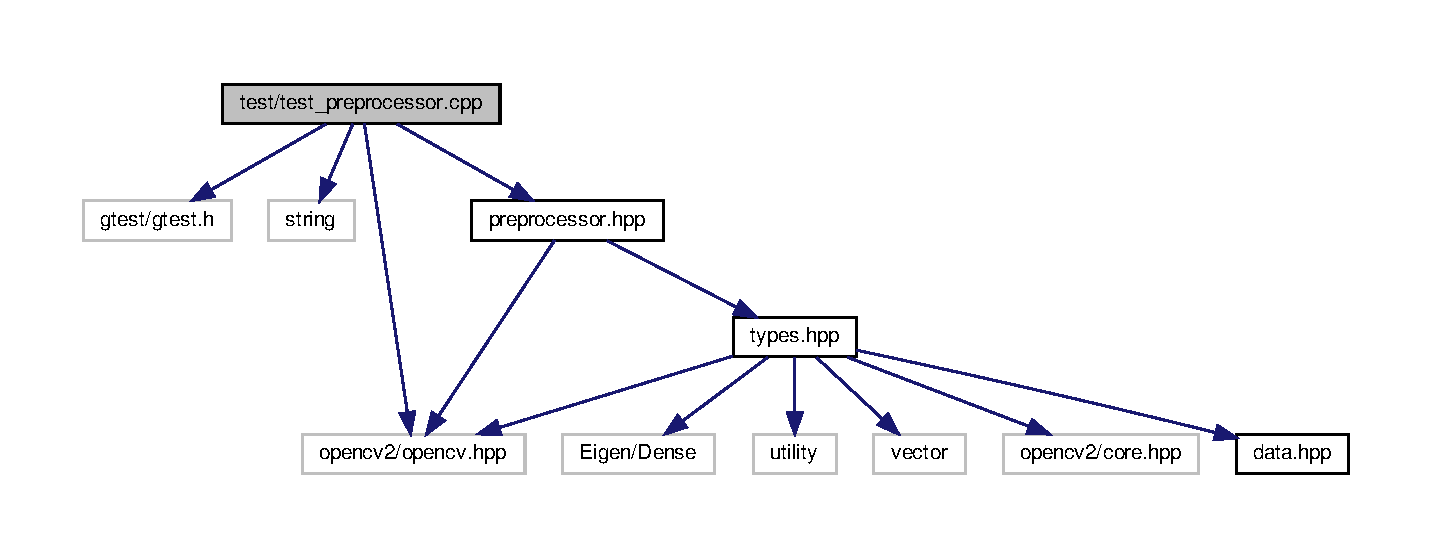
\includegraphics[width=350pt]{test__preprocessor_8cpp__incl}
\end{center}
\end{figure}
\subsection*{Functions}
\begin{DoxyCompactItemize}
\item 
\mbox{\Hypertarget{test__preprocessor_8cpp_ac0340317915a935732d825dc80c4175e}\label{test__preprocessor_8cpp_ac0340317915a935732d825dc80c4175e}} 
{\bfseries T\+E\+ST} (preprocessor\+\_\+test, image\+\_\+resize)
\item 
\mbox{\Hypertarget{test__preprocessor_8cpp_ad257765152e5fbe242b12d8223a2ead6}\label{test__preprocessor_8cpp_ad257765152e5fbe242b12d8223a2ead6}} 
{\bfseries T\+E\+ST} (preprocessor\+\_\+test, image\+\_\+resize\+\_\+no\+\_\+resize)
\end{DoxyCompactItemize}


\subsection{Detailed Description}
test file for \hyperlink{preprocessor_8cpp}{preprocessor.\+cpp} 

M\+IT License

Copyright (c) 2021 Anubhav Paras, Sakshi Kakde, Siddharth Telang

Permission is hereby granted, free of charge, to any person obtaining a copy of this software and associated documentation files (the \char`\"{}\+Software\char`\"{}), to deal in the Software without restriction, including without limitation the rights to use, copy, modify, merge, publish, distribute, sublicense, and/or sell copies of the Software, and to permit persons to whom the Software is furnished to do so, subject to the following conditions\+:

The above copyright notice and this permission notice shall be included in all copies or substantial portions of the Software.

T\+HE S\+O\+F\+T\+W\+A\+RE IS P\+R\+O\+V\+I\+D\+ED \char`\"{}\+A\+S I\+S\char`\"{}, W\+I\+T\+H\+O\+UT W\+A\+R\+R\+A\+N\+TY OF A\+NY K\+I\+ND, E\+X\+P\+R\+E\+SS OR I\+M\+P\+L\+I\+ED, I\+N\+C\+L\+U\+D\+I\+NG B\+UT N\+OT L\+I\+M\+I\+T\+ED TO T\+HE W\+A\+R\+R\+A\+N\+T\+I\+ES OF M\+E\+R\+C\+H\+A\+N\+T\+A\+B\+I\+L\+I\+TY, F\+I\+T\+N\+E\+SS F\+OR A P\+A\+R\+T\+I\+C\+U\+L\+AR P\+U\+R\+P\+O\+SE A\+ND N\+O\+N\+I\+N\+F\+R\+I\+N\+G\+E\+M\+E\+NT. IN NO E\+V\+E\+NT S\+H\+A\+LL T\+HE A\+U\+T\+H\+O\+RS OR C\+O\+P\+Y\+R\+I\+G\+HT H\+O\+L\+D\+E\+RS BE L\+I\+A\+B\+LE F\+OR A\+NY C\+L\+A\+IM, D\+A\+M\+A\+G\+ES OR O\+T\+H\+ER L\+I\+A\+B\+I\+L\+I\+TY, W\+H\+E\+T\+H\+ER IN AN A\+C\+T\+I\+ON OF C\+O\+N\+T\+R\+A\+CT, T\+O\+RT OR O\+T\+H\+E\+R\+W\+I\+SE, A\+R\+I\+S\+I\+NG F\+R\+OM, O\+UT OF OR IN C\+O\+N\+N\+E\+C\+T\+I\+ON W\+I\+TH T\+HE S\+O\+F\+T\+W\+A\+RE OR T\+HE U\+SE OR O\+T\+H\+ER D\+E\+A\+L\+I\+N\+GS IN T\+HE S\+O\+F\+T\+W\+A\+RE.

\begin{DoxyAuthor}{Author}
Anubhav Paras (\href{mailto:anubhav@umd.edu}{\tt anubhav@umd.\+edu}) 

Sakshi Kakde (\href{mailto:sakshi@umd.edu}{\tt sakshi@umd.\+edu}) 

Siddharth Telang (\href{mailto:stelang@umd.edu}{\tt stelang@umd.\+edu}) 
\end{DoxyAuthor}
\begin{DoxyVersion}{Version}
0.\+1 
\end{DoxyVersion}
\begin{DoxyDate}{Date}
2021-\/10-\/25
\end{DoxyDate}
\begin{DoxyCopyright}{Copyright}
Copyright (c) 2021 
\end{DoxyCopyright}

%--- End generated contents ---

% Index
\backmatter
\newpage
\phantomsection
\clearemptydoublepage
\addcontentsline{toc}{chapter}{Index}
\printindex

\end{document}
